% Options for packages loaded elsewhere
% Options for packages loaded elsewhere
\PassOptionsToPackage{unicode}{hyperref}
\PassOptionsToPackage{hyphens}{url}
\PassOptionsToPackage{dvipsnames,svgnames,x11names}{xcolor}
%
\documentclass[
  13,
  letterpaper,
]{report}
\usepackage{xcolor}
\usepackage[margin=1in]{geometry}
\usepackage{amsmath,amssymb}
\setcounter{secnumdepth}{4}
\usepackage{iftex}
\ifPDFTeX
  \usepackage[T1]{fontenc}
  \usepackage[utf8]{inputenc}
  \usepackage{textcomp} % provide euro and other symbols
\else % if luatex or xetex
  \usepackage{unicode-math} % this also loads fontspec
  \defaultfontfeatures{Scale=MatchLowercase}
  \defaultfontfeatures[\rmfamily]{Ligatures=TeX,Scale=1}
\fi
\usepackage{lmodern}
\ifPDFTeX\else
  % xetex/luatex font selection
  \setmainfont[]{Arial}
  \setmonofont[]{Courier New}
\fi
% Use upquote if available, for straight quotes in verbatim environments
\IfFileExists{upquote.sty}{\usepackage{upquote}}{}
\IfFileExists{microtype.sty}{% use microtype if available
  \usepackage[]{microtype}
  \UseMicrotypeSet[protrusion]{basicmath} % disable protrusion for tt fonts
}{}
\usepackage{setspace}
\makeatletter
\@ifundefined{KOMAClassName}{% if non-KOMA class
  \IfFileExists{parskip.sty}{%
    \usepackage{parskip}
  }{% else
    \setlength{\parindent}{0pt}
    \setlength{\parskip}{6pt plus 2pt minus 1pt}}
}{% if KOMA class
  \KOMAoptions{parskip=half}}
\makeatother
% Make \paragraph and \subparagraph free-standing
\makeatletter
\ifx\paragraph\undefined\else
  \let\oldparagraph\paragraph
  \renewcommand{\paragraph}{
    \@ifstar
      \xxxParagraphStar
      \xxxParagraphNoStar
  }
  \newcommand{\xxxParagraphStar}[1]{\oldparagraph*{#1}\mbox{}}
  \newcommand{\xxxParagraphNoStar}[1]{\oldparagraph{#1}\mbox{}}
\fi
\ifx\subparagraph\undefined\else
  \let\oldsubparagraph\subparagraph
  \renewcommand{\subparagraph}{
    \@ifstar
      \xxxSubParagraphStar
      \xxxSubParagraphNoStar
  }
  \newcommand{\xxxSubParagraphStar}[1]{\oldsubparagraph*{#1}\mbox{}}
  \newcommand{\xxxSubParagraphNoStar}[1]{\oldsubparagraph{#1}\mbox{}}
\fi
\makeatother

\usepackage{color}
\usepackage{fancyvrb}
\newcommand{\VerbBar}{|}
\newcommand{\VERB}{\Verb[commandchars=\\\{\}]}
\DefineVerbatimEnvironment{Highlighting}{Verbatim}{commandchars=\\\{\}}
% Add ',fontsize=\small' for more characters per line
\usepackage{framed}
\definecolor{shadecolor}{RGB}{241,243,245}
\newenvironment{Shaded}{\begin{snugshade}}{\end{snugshade}}
\newcommand{\AlertTok}[1]{\textcolor[rgb]{0.68,0.00,0.00}{#1}}
\newcommand{\AnnotationTok}[1]{\textcolor[rgb]{0.37,0.37,0.37}{#1}}
\newcommand{\AttributeTok}[1]{\textcolor[rgb]{0.40,0.45,0.13}{#1}}
\newcommand{\BaseNTok}[1]{\textcolor[rgb]{0.68,0.00,0.00}{#1}}
\newcommand{\BuiltInTok}[1]{\textcolor[rgb]{0.00,0.23,0.31}{#1}}
\newcommand{\CharTok}[1]{\textcolor[rgb]{0.13,0.47,0.30}{#1}}
\newcommand{\CommentTok}[1]{\textcolor[rgb]{0.37,0.37,0.37}{#1}}
\newcommand{\CommentVarTok}[1]{\textcolor[rgb]{0.37,0.37,0.37}{\textit{#1}}}
\newcommand{\ConstantTok}[1]{\textcolor[rgb]{0.56,0.35,0.01}{#1}}
\newcommand{\ControlFlowTok}[1]{\textcolor[rgb]{0.00,0.23,0.31}{\textbf{#1}}}
\newcommand{\DataTypeTok}[1]{\textcolor[rgb]{0.68,0.00,0.00}{#1}}
\newcommand{\DecValTok}[1]{\textcolor[rgb]{0.68,0.00,0.00}{#1}}
\newcommand{\DocumentationTok}[1]{\textcolor[rgb]{0.37,0.37,0.37}{\textit{#1}}}
\newcommand{\ErrorTok}[1]{\textcolor[rgb]{0.68,0.00,0.00}{#1}}
\newcommand{\ExtensionTok}[1]{\textcolor[rgb]{0.00,0.23,0.31}{#1}}
\newcommand{\FloatTok}[1]{\textcolor[rgb]{0.68,0.00,0.00}{#1}}
\newcommand{\FunctionTok}[1]{\textcolor[rgb]{0.28,0.35,0.67}{#1}}
\newcommand{\ImportTok}[1]{\textcolor[rgb]{0.00,0.46,0.62}{#1}}
\newcommand{\InformationTok}[1]{\textcolor[rgb]{0.37,0.37,0.37}{#1}}
\newcommand{\KeywordTok}[1]{\textcolor[rgb]{0.00,0.23,0.31}{\textbf{#1}}}
\newcommand{\NormalTok}[1]{\textcolor[rgb]{0.00,0.23,0.31}{#1}}
\newcommand{\OperatorTok}[1]{\textcolor[rgb]{0.37,0.37,0.37}{#1}}
\newcommand{\OtherTok}[1]{\textcolor[rgb]{0.00,0.23,0.31}{#1}}
\newcommand{\PreprocessorTok}[1]{\textcolor[rgb]{0.68,0.00,0.00}{#1}}
\newcommand{\RegionMarkerTok}[1]{\textcolor[rgb]{0.00,0.23,0.31}{#1}}
\newcommand{\SpecialCharTok}[1]{\textcolor[rgb]{0.37,0.37,0.37}{#1}}
\newcommand{\SpecialStringTok}[1]{\textcolor[rgb]{0.13,0.47,0.30}{#1}}
\newcommand{\StringTok}[1]{\textcolor[rgb]{0.13,0.47,0.30}{#1}}
\newcommand{\VariableTok}[1]{\textcolor[rgb]{0.07,0.07,0.07}{#1}}
\newcommand{\VerbatimStringTok}[1]{\textcolor[rgb]{0.13,0.47,0.30}{#1}}
\newcommand{\WarningTok}[1]{\textcolor[rgb]{0.37,0.37,0.37}{\textit{#1}}}

\usepackage{longtable,booktabs,array}
\newcounter{none} % for unnumbered tables
\usepackage{calc} % for calculating minipage widths
% Correct order of tables after \paragraph or \subparagraph
\usepackage{etoolbox}
\makeatletter
\patchcmd\longtable{\par}{\if@noskipsec\mbox{}\fi\par}{}{}
\makeatother
% Allow footnotes in longtable head/foot
\IfFileExists{footnotehyper.sty}{\usepackage{footnotehyper}}{\usepackage{footnote}}
\makesavenoteenv{longtable}
\usepackage{graphicx}
\makeatletter
\newsavebox\pandoc@box
\newcommand*\pandocbounded[1]{% scales image to fit in text height/width
  \sbox\pandoc@box{#1}%
  \Gscale@div\@tempa{\textheight}{\dimexpr\ht\pandoc@box+\dp\pandoc@box\relax}%
  \Gscale@div\@tempb{\linewidth}{\wd\pandoc@box}%
  \ifdim\@tempb\p@<\@tempa\p@\let\@tempa\@tempb\fi% select the smaller of both
  \ifdim\@tempa\p@<\p@\scalebox{\@tempa}{\usebox\pandoc@box}%
  \else\usebox{\pandoc@box}%
  \fi%
}
% Set default figure placement to htbp
\def\fps@figure{htbp}
\makeatother





\setlength{\emergencystretch}{3em} % prevent overfull lines

\providecommand{\tightlist}{%
  \setlength{\itemsep}{0pt}\setlength{\parskip}{0pt}}



 


\usepackage{setspace}
\usepackage{microtype}
\emergencystretch=3em
\makeatletter
\@ifpackageloaded{bookmark}{}{\usepackage{bookmark}}
\makeatother
\makeatletter
\@ifpackageloaded{caption}{}{\usepackage{caption}}
\AtBeginDocument{%
\ifdefined\contentsname
  \renewcommand*\contentsname{Table of contents}
\else
  \newcommand\contentsname{Table of contents}
\fi
\ifdefined\listfigurename
  \renewcommand*\listfigurename{List of Figures}
\else
  \newcommand\listfigurename{List of Figures}
\fi
\ifdefined\listtablename
  \renewcommand*\listtablename{List of Tables}
\else
  \newcommand\listtablename{List of Tables}
\fi
\ifdefined\figurename
  \renewcommand*\figurename{Figure}
\else
  \newcommand\figurename{Figure}
\fi
\ifdefined\tablename
  \renewcommand*\tablename{Table}
\else
  \newcommand\tablename{Table}
\fi
}
\@ifpackageloaded{float}{}{\usepackage{float}}
\floatstyle{ruled}
\@ifundefined{c@chapter}{\newfloat{codelisting}{h}{lop}}{\newfloat{codelisting}{h}{lop}[chapter]}
\floatname{codelisting}{Listing}
\newcommand*\listoflistings{\listof{codelisting}{List of Listings}}
\makeatother
\makeatletter
\makeatother
\makeatletter
\@ifpackageloaded{caption}{}{\usepackage{caption}}
\@ifpackageloaded{subcaption}{}{\usepackage{subcaption}}
\makeatother
\usepackage{bookmark}
\IfFileExists{xurl.sty}{\usepackage{xurl}}{} % add URL line breaks if available
\urlstyle{same}
\hypersetup{
  pdftitle={Bayesian Inference for Biologists},
  pdfauthor={Nick Green},
  colorlinks=true,
  linkcolor={blue},
  filecolor={Maroon},
  citecolor={Blue},
  urlcolor={Blue},
  pdfcreator={LaTeX via pandoc}}


\title{Bayesian Inference for Biologists}
\author{Nick Green}
\date{August 15, 2026}
\begin{document}
\maketitle

\renewcommand*\contentsname{Table of contents}
{
\setcounter{tocdepth}{2}
\tableofcontents
}

\setstretch{1.3}
\bookmarksetup{startatroot}

\chapter*{Welcome}\label{welcome}
\addcontentsline{toc}{chapter}{Welcome}

\markboth{Welcome}{Welcome}

These notes accompany \textbf{BIOL 7950: Bayesian Inference for
Biologists} at Kennesaw State University.

The goal of this course is to introduce Bayesian statistical thinking
and modern Bayesian analysis for biological data.

\section*{Course organization}\label{course-organization}
\addcontentsline{toc}{section}{Course organization}

\markright{Course organization}

The book is organized into three parts:

\begin{enumerate}
\def\labelenumi{\arabic{enumi}.}
\tightlist
\item
  Foundations: introduces the basic ideas behind Bayesian inference,
  Bayes' rule, and how Bayesian inference differs from frequentist
  inference. Also introduces some key aspects of working with Bayesian
  models in R and JAGS.
\item
  Bayesian analyses in R and JAGS: demonstrates Bayesian versions of
  common models for biology like linear models, GLMs, and nonlinear
  models.
\item
  Special applications: demonstrates some situations where Bayesian
  methods really shine, like mark-recapture and state space models.
\end{enumerate}

This book is always a work in progress and I welcome constructive
criticism and feedback. You can get in touch with me by
\href{mailto:ngreen62@kennesaw.edu}{email}, on
\href{https://bsky.app/profile/greenquanteco.bsky.social}{Bluesky
({[}at{]}greenquanteco)}, and \href{https://x.com/GreenQuantEco}{Twitter
({[}at{]}GreenQuantEco)}.

Visit the \href{https://greenquanteco.github.io/}{lab website} for more
information about Dr.~Green's other courses and QuantEco lab research!

\part{Introduction to Bayesian inference}

If it feels backwards, that's because it is.

\chapter{Introduction: Modes of inference}\label{sec-intro}

\section{Motivation: hypothesis testing in
biology}\label{motivation-hypothesis-testing-in-biology}

\section{\texorpdfstring{Null hypothesis significance testing and
\emph{p}-values}{Null hypothesis significance testing and p-values}}\label{null-hypothesis-significance-testing-and-p-values}

\section{Maximum likelihood estimation
(MLE)}\label{maximum-likelihood-estimation-mle}

\section{Bayes' Theorem}\label{bayes-theorem}

\chapter{Probability and Bayes' theorem}\label{sec-bayes}

\section{Bayesian thinking}\label{bayesian-thinking}

\subsection{Priors}\label{priors}

\subsection{Evidence (Data)}\label{evidence-data}

\subsection{Posteriors}\label{posteriors}

\section{Updating beliefs and Bayes'
factors}\label{updating-beliefs-and-bayes-factors}

\chapter{Introduction to JAGS and MCMC}\label{sec-jags}

\section{Overview and objectives}\label{overview-and-objectives}

This week we will explore the basics of JAGS, a common software package
for fitting models under Bayesian inference. Despite its conceptual
elegance, Bayesian inference in practice is far more computationally
intensive than frequentist inference. While computational methods for
frequentist inference were optimized decades ago, methods for Bayesian
inference are growing and improving rapidly. For these reasons most
entry-level statistical packages such as R or SAS rely on extensions or
separate programs to conduct the computations for Bayesian methods. In
this module we will go over the steps of running a simple model in JAGS
from R. This workflow will serve as a template for more complicated
analyses throughout the semester.

\textbf{By the end of this module you should be able to:}

\begin{enumerate}
\def\labelenumi{\arabic{enumi}.}
\tightlist
\item
  Install R, JAGS, and R packages.
\item
  Call and run JAGS from R.
\item
  Specify simple models in the BUGS/JAGS language.
\item
  Interpret outputs from JAGS to make inferences about biological
  systems.
\end{enumerate}

For this module you will need:

\begin{Shaded}
\begin{Highlighting}[]
\FunctionTok{library}\NormalTok{(R2jags)}
\FunctionTok{library}\NormalTok{(rjags)}
\end{Highlighting}
\end{Shaded}

\section{Preliminary steps}\label{preliminary-steps}

\subsection{Installing R}\label{installing-r}

R is a software package used primarily for statistical analysis, as well
as a programming language used to interact with the program. It is
widely used in academia, government, and private industry for data
analysis. Many on-campus computers at KSU already have R installed on
them.

First, install the latest version of R from
\href{https://cran.r-project.org/mirrors.html}{here} (accessed
2026-07-24). Select a mirror (download server) from the list. You will
be taken to a page where you will select the version of R that
corresponds to your operating system. Click on the link for your OS and
follow the instructions from there. Like many programs from the
internet, R comes with an installer that will largely take care of
everything automatically. Just let the installer run and accept the
default options.

Optionally, you can install RStudio. It can be downloaded from
\href{https://docs.posit.co/ide/user/\#rstudio-ide-oss-downloads}{here}
(accessed 2026-07-24). As with R, select the version that corresponds to
your operating system. As you did when you installed R above, just let
the installer run and accept the default options. In this class we will
use the base R graphical user interface (GUI) for simplicity, but some
people prefer RStudio.

This course assumes some basic familiarity with R and R programming;
alternatively, some level of comfort with any command-line or
programming interface. If you can write an Excel formula, you will
probably be fine. If you need an introduction to or refresher on R,
there are many free tutorials for R available on the web.

\subsection{Install JAGS}\label{install-jags}

JAGS, short for ``Just Another Gibbs Sampler'', is a program for fitting
models using Markov chain Monte Carlo (Plummer 2003). It is one of the
most popular programs for Bayesian inference.

JAGS is hosted on
\href{https://sourceforge.net/projects/mcmc-jags/}{SourceForge here}
(accessed 2023-01-05). Click the big green download button. After the
program downloads, follow the on-screen instructions for the
installation process. JAGS comes with its own installer much like any
other program you download from the internet.

\subsection{Installing R packages}\label{installing-r-packages}

JAGS is mainly designed to be called from other programs, so it doesn't
have a GUI. In order to call JAGS from R, you will need two packages:
rjags (Plummer 2022) and R2jags (Su and Yajima 2021). Install these in R
using the following commands. Click Yes or OK on any pop-up messages
from R.

\begin{Shaded}
\begin{Highlighting}[]
\FunctionTok{install.packages}\NormalTok{(}\StringTok{"rjags"}\NormalTok{)}
\FunctionTok{install.packages}\NormalTok{(}\StringTok{"R2jags"}\NormalTok{)}
\end{Highlighting}
\end{Shaded}

These packages will be installed to your personal R library. This means
that they are only available under your operating system profile
(log-in). If someone else logs into the same machine, they may have R
installed but won't have any add-on packages installed. This is because
packages are stored in a folder tied to your operating system profile.

These packages are also specific to the version of R used to install
them. Each version of R installed on your machine has its own library,
or folder containing add-on packages. If you update R, you will need to
reinstall any add-on packages.

\section{Markov chain Monte Carlo sampling
(MCMC)}\label{markov-chain-monte-carlo-sampling-mcmc}

\subsection{Integral calculus is hard}\label{integral-calculus-is-hard}

In frequentist inference, most statistical models can be fitted by
calculating model parameters that produce the best fit to the data. For
example, for ordinary linear models, there is always a way to solve for
the values of the coefficients that minimize the sum of squared errors.
For other models, there is typically a closed-form solution or a robust
approximation algorithm for finding optimal parameter values. In most
programs for statistical analysis, including R, these calculations take
place internally and the user has little, if any, exposure to them.

In modern statistical programs (including R), many models are fit by a
method called \textbf{maximum likelihood}: finding the parameter values
that result in the greatest value of the likelihood function. The
likelihood function is an expression of how likely the observed data are
conditional on the parameter values. In practice, most software actually
minimizes the negative of the logarithm of the likelihood function (the
``negative log-likelihood''). This is more convenient mathematically,
and doesn't really matter for the end user.

The take home message of the above paragraphs is that in frequentist
inference, the model parameters are found by maximum likelihood (ML),
also known as maximum likelihood estimation (MLE). MLE works by solving
or approximating a solution to find optimal parameter values.

In Bayesian inference, it is rarely possible to solve for model
parameters. The equations that would have to be solved usually have no
closed-form solution, and are computationally intractable. These usually
take the form of high-dimensional integrals. Given Bayes' theorem:

\[p\left(\theta|x\right)=\frac{p\left(x|\theta\right)p\left(\theta\right)}{p\left(x\right)}\]

where \(\theta\) is the set of model parameters (i.e., the hypothesis
\(H\)) and \(x\) is the data (i.e., the evidence \(E\)), the numerator
is usually straightforward to calculate (it is the likelihood function
time scaled by the prior probability of the parameter values).

The denominator, however, is actually very hard to calculate. It is
defined as an integral over as many dimensions as there are parameters,
which has to be computed over all possible parameter values, for all
parameters, which can't be done in a closed form way except for the
simplest models. This means that optimization methods such as
Newton-Raphson, which work well for finding a single best-fitting
parameter value, cannot generally be used to solve the Bayesian problem
because Bayesian inference requires integrating over the entire
posterior distribution rather than finding a single optimum.

The solution for fitting Bayesian models is to use a process called
\textbf{Markov chain Monte Carlo (MCMC)}. This is a class of methods
that combine \textbf{Markov chains} (a kind of sequence generating
process) with random sampling (the Monte Carlo part, named after a
European city famous for its casinos). These methods use probabilistic
sampling to avoid having to compute that integral explicitly and instead
approximate the posterior distributions by sampling from them.

A Markov chain is a stochastic process where some state (like a
parameter value) changes over time according to probabilistic rules.
Usually ``time'' is considered to be discrete, so the chain proceeds in
``steps''. In a Markov chain, the state at the next step depends only on
the state at the current step. In this way, the chain has a very weak
memory and thus states at steps that are very far apart are usually
considered to be nearly independent (usually).

\subsection{Gibbs sampling}\label{gibbs-sampling}

There are many kinds of MCMC algorithms. One of the most common is a
method called \textbf{Gibbs sampling}. It is the ``GS'' in ``BUGS'' and
``JAGS''. Gibbs sampling is actually a special case of a broader class
of methods called Metropolis-Hastings methods. So, Gibbs sampling is a
subset of Metropolis-Hastings sampling, which is a subset of MCMC
methods, which are an alternative to maximum likelihood).

The basic procedure is as follows:

\begin{enumerate}
\def\labelenumi{\arabic{enumi}.}
\tightlist
\item
  Start with an initial value for each parameter in the set of
  parameters \(\theta\).
\item
  Update the value of each parameter, conditional on the current value
  of the other parameters. This updating is done by drawing from the
  full conditional posterior distribution of the data given the other
  parameter values (despite using the phrase ``maxmizes the
  likelihood'', this is NOT MLE).
\item
  Use the updated values as the starting point for the next step.
\item
  Repeat many, many times until the chain converged to the joint
  posterior distribution.
\end{enumerate}

This basic procedure is a very simplified explanation, and glosses over
a lot of math. But, it gives you the basic idea. The full details are
not necessary to use MCMC, and are beyond the scope of this course.

\subsection{What you need to know about
MCMC}\label{what-you-need-to-know-about-mcmc}

The more practical things you need to know are about MCMC are:

\textbf{Chains can take many steps to find the posterior distribution}

MCMC chains often start at initial parameter values that are essentially
random and not representative of the posterior distribution. So, we
discard the first part of a chain as burn-in. Many people use 10\% or
20\% as burn-in, but there is no universally agreed-upon rule. MCMC
chains often need to be very long, many thousands of steps, to find
robust approximations of the posterior distributions of all the
parameters. In my own work I usually use \(\geq\) 100,000 steps, or
\(\geq\) 250,000 for complicated models.

\textbf{Chains are autocorrelated}

The values in an MCMC chain can be correlated with values in nearby
steps; in other words, chains are autocorrelated. To reduce the
influence of this autocorrelation, some people \textbf{thin} the chains
by only keeping every so many observations. Ratios of 1 in 20 or 1 in
100 are common. I usually thin my chains so that they end up with 1000
to 2000 posterior values. Note that in some software (e.g., stan),
thinning is not recommended. However, thinning is still standard
practice for using JAGS.

\textbf{Chains might not find the posterior distribution}

There is no guarantee that and MCMC chain will adequately explore the
correct posterior distribution. Even if the initial prior distribution
is appropriate and the data robust, there are still some chain
pathologies to watch out for. Chains can fail to converge; become
trapped near a local mode (but not the global mode); or mix poorly (the
chains do not agree).

For this reason, most MCMC analyses use multiple chains. If the chains
converge to the same stationary distribution, then we say the chains
have converged. Most analyses use 3 chains, but some researchers use
other numbers.

\textbf{MCMC model fitting requires tuning}

The parameters of the MCMC process often need to be optimized for an
analysis. This process is referred to as \textbf{tuning}. Some people
will try fitting models with different numbers of chains, different
chain lengths, different thinning intervals, and different burn-in
periods until they find a consensus. In my experience, this is usually
overkill. My approach (which is very common) is to simply use a
conservative set of tuning parameters---that is, a set of tuning
parameters that is probably overkill and is thus very likely to find a
good solution. As they say, brute force always works if you use enough.

\textbf{One chain or many chains?}

Some people argue that you should use 1 very long chain instead of 3
shorter chains. For example, 1 chain of 300,000 iterations instead of 3
chains of 100,000 iterations. Both approaches would get you the same
number of posterior samples. In my own work I prefer the multiple chain
approach, mostly because this helps avoid issues related to the choice
of initial value.

\section{JAGS workflow}\label{jags-workflow}

The workflow for fitting Bayesian models in JAGS, called from R, is
summarized in the flowchart below. Most of the steps take place within
R, using R code (central grey box).

\begin{figure}

\caption{\label{fig-jags-workflow}Workflow for fitting Bayesian models
in JAGS using R. Data are first imported into R and pre-processed by
formatting the data, specifying initial parameter values, and choosing
MCMC settings. These inputs are passed to the \texttt{jags()} function,
which calls a model written in the JAGS language. JAGS fits the model
using MCMC and returns a results object to R, where convergence is
assessed and the posterior distributions are used for model selection,
plotting, and interpretation.}

\centering{

\pandocbounded{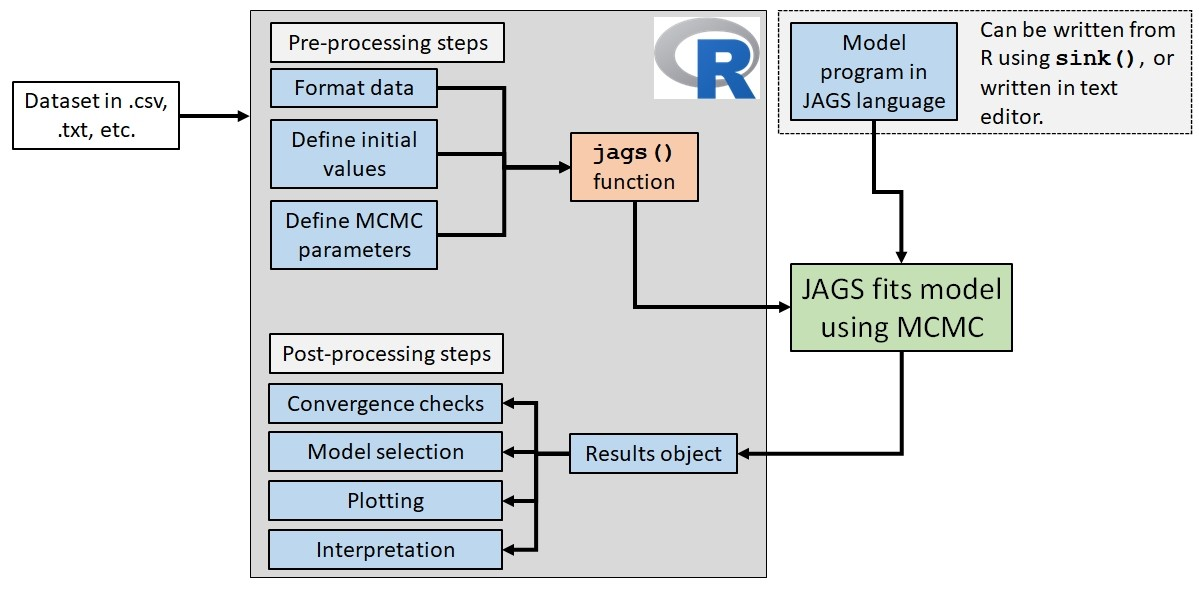
\includegraphics[keepaspectratio,alt={Flowchart showing the workflow for fitting Bayesian models in JAGS using R. A dataset is imported into R, where pre-processing includes formatting the data, defining initial values, and specifying MCMC parameters. These inputs are passed to the `jags()` function, while a model written in the JAGS language is supplied separately. JAGS fits the model using Markov chain Monte Carlo and returns a results object to R. The results are then used for convergence diagnostics, model selection, plotting, and biological interpretation.}]{chapters/../images/04-01.jpg}}

}

\end{figure}%

\subsection{Step 1: Data import}\label{step-1-data-import}

The dataset should be set up for import to R just like it would for a
frequentist analysis. Ideally this is in a plain-text format like
comma-separated values (.csv file) or tab-delimited values (.txt). The
data should follow ``tidy'' data principles (Broman and Woo 2018;
Wickham 2014), where each observation is a row, and each variable
(column) contains only one kind of value. Note that some common R
conventions, like using character strings to identify levels of a
factor, are not compatible with the JAGS language. These issues will be
addressed in the next step.

\subsection{Step 2: Pre-processing
steps}\label{step-2-pre-processing-steps}

Before fitting a model in JAGS, we need to set up some objects that will
tell JAGS what to do.

\subsubsection{Format data}\label{format-data}

Data in R are usually held in a data frame. In order to go to JAGS, the
data need to be repackaged into a list. Some kinds of data need to be
reformatted:

\begin{itemize}
\tightlist
\item
  Character strings need to be replaced with integers. For example, a
  factor with levels \texttt{level1}, \texttt{level2}, and
  \texttt{level3} needs to be recoded to \texttt{1}, \texttt{2}, and
  \texttt{3}. It is very important that you record how the values were
  recoded.
\item
  Values intended to be integers (e.g., counts) should be rounded (e.g.,
  \texttt{round(x,\ 0)}). This is not always necessary, but sometimes
  non-integer values can sneak in if the data file was not saved
  correctly. Doing this is an extra safety check.
\item
  Variable names should be made simple, and not include any spaces.
\end{itemize}

\subsubsection{Define initial values}\label{define-initial-values}

Any stochastic value in the model---a model \textbf{parameter}---must be
supplied with an initial value for each chain. These values should be
drawn randomly from the prior distribution. The most common way I've
seen is to write a function in R that randomly draws initial values and
stores them in an object with the following structure:

\begin{figure}

\caption{\label{fig-jags-inits}Structure of the initial values object
supplied to JAGS. The object is a list with one element for each MCMC
chain. Each element is itself a named list containing one initial value
for every model parameter. This allows each chain to begin from a
different set of starting parameter values.}

\centering{

\pandocbounded{\includegraphics[keepaspectratio,alt={Diagram illustrating the structure of the initial values object passed to JAGS. The outer object is a list whose elements correspond to MCMC chains ({[}{[}1{]}{]}, {[}{[}2{]}{]}, ..., {[}{[}k{]}{]}). Each chain contains a named list with one entry for each model parameter (for example, param1 and param2), specifying the initial values used to start that chain. The structure emphasizes that each chain has its own complete set of initial parameter values.}]{chapters/../images/04-02.jpg}}

}

\end{figure}%

\subsubsection{Set MCMC parameters}\label{set-mcmc-parameters}

Markov-chain Monte Carlo (MCMC) is inherently a stochastic process, so
fitting models with MCMC involves some tuning. This means adjusting the
parameters of the run so that the results make sense and are consistent
from run to run. The following parameters need to be set for JAGS run:

\begin{longtable}[]{@{}
  >{\raggedright\arraybackslash}p{(\linewidth - 4\tabcolsep) * \real{0.3056}}
  >{\centering\arraybackslash}p{(\linewidth - 4\tabcolsep) * \real{0.4444}}
  >{\raggedright\arraybackslash}p{(\linewidth - 4\tabcolsep) * \real{0.2500}}@{}}
\caption{Typical MCMC tuning parameters used when fitting Bayesian
models in JAGS.}\label{tbl-mcmc-parameters}\tabularnewline
\toprule\noalign{}
\begin{minipage}[b]{\linewidth}\raggedright
Parameter
\end{minipage} & \begin{minipage}[b]{\linewidth}\centering
Typical settings
\end{minipage} & \begin{minipage}[b]{\linewidth}\raggedright
Meaning
\end{minipage} \\
\midrule\noalign{}
\endfirsthead
\toprule\noalign{}
\begin{minipage}[b]{\linewidth}\raggedright
Parameter
\end{minipage} & \begin{minipage}[b]{\linewidth}\centering
Typical settings
\end{minipage} & \begin{minipage}[b]{\linewidth}\raggedright
Meaning
\end{minipage} \\
\midrule\noalign{}
\endhead
\bottomrule\noalign{}
\endlastfoot
Number of chains & \(\geq3\) & Number of independent MCMC chains.
Multiple chains are run to reduce the influence of initial values and
reduce the chances of getting stuck in local optima. \\
Number of iterations & \(\geq50000\) & Number of steps in each MCMC
chain. \\
Burn-in & 20\% of iterations & The initial iterations of each chain are
discarded as \emph{burn-in} to reduce the influence of initial values
and increase the likelihood of chain convergence. \\
Thinning interval & \(\geq20\) or \(\geq100\) & MCMC chains are
\emph{thinned} by keeping only iterations separated by the thinning
interval. This reduces the influence of autocorrelation within a
chain. \\
\end{longtable}

For example, a researcher might run a model with 3 chains of 100,000
iterations, a burn-in period of 20,000, and a thinning interval of 100.
They would end up with \(3\times(100000-20000) / 100 = 2400\) samples
from the posterior distribution of each parameter. These 2,400 samples
would be the basis for inference about the parameters. I try to make
sure that I have at least 1000 to 2000 posterior samples for each
parameter, but there is no universally agreed-upon rule.

Finally, the parameters to be ``monitored'' by JAGS need to be
identified as a character vector. These are the parameters whose
posterior distributions JAGS will keep track of. For example, if you fit
a regression model, you need to tell JAGS to monitor the intercept,
slope, and residual variance term. Otherwise, JAGS will fit the model
but not return any posterior chains.

\subsection{Step 3: Writing the model
file}\label{step-3-writing-the-model-file}

Models in JAGS are coded using a dialect of the BUGS modeling language
(Lunn et al.~2000). The model specification must define the prior
distribution of each parameter, the relationships between the parameters
and the data, and any derived quantities of interest (more on this
later). JAGS reads a model specification from a text file (.txt) or BUGS
file (.bug). I prefer to use text files because they can be written
easily from within R, and read on any machine. The model text file, as
its file path, is provided to the \texttt{jags()} function that calls
JAGS from R so JAGS knows where to look.

As we'll see later, the BUGS/JAGS language is declarative, not
imperative. This means that a model is specified by defining how the
variables relate to each other, not by issuing a series of instructions
to be executed in order.The order of most model statements does not
determine the order of execution, because JAGS uses them to construct a
directed acyclic graph of dependencies.

This can be a bit confusing to new users. Most of us are used to writing
code like this:

\begin{Shaded}
\begin{Highlighting}[]
\NormalTok{Do thing 1}

\NormalTok{Do thing 2}

\NormalTok{Do thing 3}
\end{Highlighting}
\end{Shaded}

But JAGS code works like this:

\begin{Shaded}
\begin{Highlighting}[]
\NormalTok{Object A depends on Object B}

\NormalTok{Values in Object B are drawn from a normal distribution with mean = 2 and sd = 1}

\NormalTok{Variable C is calculated from Object A}
\end{Highlighting}
\end{Shaded}

\subsection{Step 4: Running JAGS from
R}\label{step-4-running-jags-from-r}

All of the objects and files produced in the pre-processing steps are
included as inputs to the function \texttt{jags()}. This function will
package everything up and send it to JAGS. JAGS will then run the model,
occasionally printing status updates to the R console. Depending on the
size of the dataset and the complexity of the model, this step can eat
up a lot of memory and processor capacity. So, save everything before
you start JAGS!

When JAGS is done it will return the results to R so they can be saved
in an object. This is why you should always assign the output of
\texttt{jags()} to an object:

\begin{Shaded}
\begin{Highlighting}[]
\NormalTok{resultobject }\OtherTok{\textless{}{-}} \FunctionTok{jags}\NormalTok{(...)}
\end{Highlighting}
\end{Shaded}

There is nothing so frustrating as waiting 3 days for a model to run
only to find that the output wasn't saved anywhere!

\subsection{Step 5: Post-processing
steps}\label{step-5-post-processing-steps}

After you run the model in JAGS and get an output, the real work begins.
Unlike a frequentist model that has essentially everything calculated
for you automatically, a Bayesian model output needs to be carefully
inspected. This is, in no small part, because there are no universally
accepted criteria for model acceptance or rejection the way there are
for frequentist models.

Every project's workflow is a little different, but most involve at
least these steps:

\begin{itemize}
\tightlist
\item
  \textbf{Convergence:} checking to see whether the MCMC chains
  converged on the same posterior distribution. Basically, this means
  that the chains agree with each other . If chains do not agree, this
  could indicate any number of problems: (1) the model needs to be run
  for longer; (2) the tuning parameters need to be adjusted; (3) the
  model is poorly defined or does not fit; (4) the initial values have a
  lot of influence; or some combination of these (or another problem all
  together\ldots here be dragons).
\item
  \textbf{Model selection:} Just as in frequentist inference, we often
  fit several models representing alternative hypotheses, and try to
  identify which model best fits the data. JAGS calculates a metric
  called the deviance information criterion (DIC) that can be used in a
  manner analogous to the Akaike information criterion (AIC) .
\item
  \textbf{Plotting:} Plotting the model and its predictions (and
  uncertainty) is one of the best ways to present the results of any
  analysis. Predicted values and the uncertainty surrounding those
  predictions are trivially easy to calculate with posterior
  distributions---because we have thousands of samples from the
  posterior distribution of each parameter, we can automatically get a
  distribution of the response variable conditional on those
  distributions. This neatly solves the error propagation problem
  inherent in frequentist models .
\item
  \textbf{Interpretation:} The values from each chain are samples from
  the posterior distributions of each parameter. These samples, and
  summaries thereof, can be used to make inferences about the
  parameters.
\end{itemize}

\section{Specifying models in JAGS}\label{specifying-models-in-jags}

JAGS has its own language for programming models. This language is
almost identical to the language developed for an older family of
programs, WinBUGS and OpenBUGS (``BUGS'' is short for ``Bayesian
inference Using Gibbs Sampling''). So, almost any code example written
for WinBUGS or OpenBUGS should also work for JAGS . Much of the syntax
of JAGS is like the syntax of R, so R users often have an easy time
learning BUGS and JAGS.

The biggest difference between the JAGS and R languages are in how
commands are interpreted. R is usually imperative: commands are executed
in the order in which they are written, one after another. JAGS,
however, is declarative: commands define the relationships between
objects and parameters. This difference can be very confusing to new
users, especially users without much programming experience.

One way to think of a JAGS program is as the definition of a directed
acyclic graph (DAG). This is a way of representing the connections
between components of a system (like a statistical model). For example,
the directed acyclic graph for an ordinary linear regression model is
shown below:

\begin{figure}

\caption{\label{fig-linear-dag}Directed acyclic graph (DAG) for a
Bayesian linear regression model. The intercept (\(\beta_0\)), slope
(\(\beta_0\)), and predictor (\(x_i\)) determine the expected value of
the response, \(E\left(y_i\right)\). The observed response \(y_i\)) is
generated from this expectation together with the residual standard
deviation \(\sigma_{res}\).}

\centering{

\pandocbounded{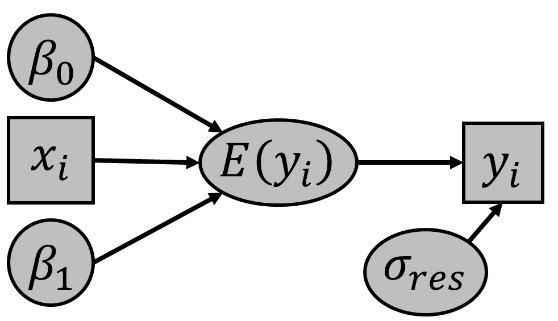
\includegraphics[keepaspectratio,alt={Directed acyclic graph representing a Bayesian linear regression model. Circular nodes represent model parameters and square nodes represent observed variables. The intercept parameter beta-zero, slope parameter beta-one, and predictor x-sub-i all point to the expected response E of y-sub-i. The expected response then points to the observed response y-sub-i, which also depends on the residual standard deviation sigma-sub-res. The arrows indicate the dependency structure used to define the model.}]{chapters/../images/04-03.jpg}}

}

\end{figure}%

The graph shows that each observed \(y\) value \(y_i\) is determined by
its expected value \(E\left(y_i\right)\) and the residual standard
deviation \(\sigma_{res}\). The expected value is determined by the
observed \(x\) value \(x_i\) and the model parameters \(\beta_0\) and
\(\beta_0\).

The key components of JAGS code are deterministic nodes and stochastic
nodes.

\textbf{Deterministic nodes} have no random component. They are defined
with a \texttt{\textless{}-}, just like assignment in R.

\begin{Shaded}
\begin{Highlighting}[]
\NormalTok{eta[i] \textless{}{-} beta0 + beta1 * x[i]}
\end{Highlighting}
\end{Shaded}

Stochastic nodes have a random component. They are defined with a
\texttt{\textasciitilde{}}. Think of this symbol as ``distributed as''.

\begin{Shaded}
\begin{Highlighting}[]
\NormalTok{y[i] \textasciitilde{} dnorm(eta[i], tau[i])}
\end{Highlighting}
\end{Shaded}

One important thing to remember is that each node can only be defined
\textbf{once}. This is because defining a node more than once is
tantamount to having a cycle in the graph, which is not allowed in JAGS.

Another key difference between R and JAGS is that R is vectorized, while
JAGS is not. For example, the following R code is valid, no matter how
many elements are in x:

\begin{Shaded}
\begin{Highlighting}[]
\NormalTok{eta \textless{}{-} 0.5 + 2 * x}
\end{Highlighting}
\end{Shaded}

The same expression or relationship in JAGS must be coded in a
\texttt{for()} loop:

\begin{Shaded}
\begin{Highlighting}[]
\NormalTok{for(i in 1:n)\{eta[i] \textless{}{-} 0.5 + 2 * x[i]\}}
\end{Highlighting}
\end{Shaded}

When expressions like this are used, the size of the deterministic node
(\texttt{eta}) is defined implicitly by the loop length \texttt{n}. This
can be a bit confusing if you are used to declaring object sizes
explicitly.

\section{\texorpdfstring{Example analysis: two-sample
\emph{t}-test}{Example analysis: two-sample t-test}}\label{example-analysis-two-sample-t-test}

Let's put all of this together and run a simple analysis---a two-sample
\emph{t}-test---in JAGS. We will simulate our own data so that we can
check the results.

Some of this tutorial is inspired by chapter 7 of Kéry (2010), but
implemented differently.

First, simulate two sets of normally distributed values with known means
(\texttt{mu1} and \texttt{mu2}) and SD (\texttt{sigma1} and
\texttt{sigma2}):

\begin{Shaded}
\begin{Highlighting}[]
\FunctionTok{set.seed}\NormalTok{(}\DecValTok{123}\NormalTok{)}
\CommentTok{\# true parameters}
\NormalTok{n }\OtherTok{\textless{}{-}} \DecValTok{20}
\NormalTok{mu1 }\OtherTok{\textless{}{-}} \DecValTok{10}
\NormalTok{mu2 }\OtherTok{\textless{}{-}} \DecValTok{20}
\NormalTok{sigma1 }\OtherTok{\textless{}{-}} \DecValTok{3}
\NormalTok{sigma2 }\OtherTok{\textless{}{-}} \DecValTok{6}

\CommentTok{\# draw values}
\NormalTok{y1 }\OtherTok{\textless{}{-}} \FunctionTok{rnorm}\NormalTok{(n, mu1, sigma1)}
\NormalTok{y2 }\OtherTok{\textless{}{-}} \FunctionTok{rnorm}\NormalTok{(n, mu2, sigma2)}

\CommentTok{\# assemble data frame}
\CommentTok{\# note grouping variable x is }
\CommentTok{\# coded as a number because}
\CommentTok{\# that\textquotesingle{}s what works in JAGS}
\NormalTok{y }\OtherTok{\textless{}{-}} \FunctionTok{c}\NormalTok{(y1, y2)}
\NormalTok{x }\OtherTok{\textless{}{-}} \FunctionTok{rep}\NormalTok{(}\DecValTok{1}\SpecialCharTok{:}\DecValTok{2}\NormalTok{, }\AttributeTok{each=}\NormalTok{n)}
\end{Highlighting}
\end{Shaded}

Next, we need to define the model file. There are several ways to code
the two-sample \emph{t}-test---we'll use the means parameterization.
\textbf{Means parameterization} refers to the fact that the model is
specified in terms of the group-level means, rather than in terms of the
between-group effect. This is a little different than the way that most
frequentist methods describe models. We'll try the effects
parameterization later.

\begin{Shaded}
\begin{Highlighting}[]
\CommentTok{\# means parameterization of two{-}sample t{-}test}
\CommentTok{\# with equal variances}
\NormalTok{mod.name }\OtherTok{\textless{}{-}} \StringTok{"jags\_ttest\_01.txt"}
\FunctionTok{sink}\NormalTok{(mod.name)}
\FunctionTok{cat}\NormalTok{(}\StringTok{"}
\StringTok{    model\{}
\StringTok{        \# priors}
\StringTok{        }
\StringTok{        for(i in 1:2)\{}
\StringTok{            \#\# group means}
\StringTok{            mu[i] \textasciitilde{} dnorm(0, 0.001)}
\StringTok{            \#\# residual and precision}
\StringTok{            sigma[i] \textasciitilde{} dunif(0.0001, 10)}
\StringTok{            tau[i] \textless{}{-} 1 / (sigma[i]\^{}2)}
\StringTok{        \}\#i}

\StringTok{        \# likelihood}
\StringTok{        for(i in 1:n)\{}
\StringTok{            y[i] \textasciitilde{} dnorm(mu[x[i]], tau[x[i]])}
\StringTok{        \}\#i}

\StringTok{        \# derived parameters}
\StringTok{        effect \textless{}{-} mu[2] {-} mu[1]}
\StringTok{    \}\#model}

\StringTok{"}\NormalTok{, }\AttributeTok{fill=}\ConstantTok{TRUE}\NormalTok{)}
\FunctionTok{sink}\NormalTok{()}
\end{Highlighting}
\end{Shaded}

The pair of \texttt{sink()} commands will write everything between them
to the specified file\ldots in this case, a text file in the R home
directory.

Next, make a vector of names of parameters to monitor. These parameters
will be reported in the results table at the end.

\begin{Shaded}
\begin{Highlighting}[]
\CommentTok{\# parameters to monitor}
\NormalTok{params }\OtherTok{\textless{}{-}} \FunctionTok{c}\NormalTok{(}\StringTok{"mu"}\NormalTok{, }\StringTok{"effect"}\NormalTok{, }\StringTok{"sigma"}\NormalTok{)}
\end{Highlighting}
\end{Shaded}

Set MCMC parameters: number of iterations, length of burn-in, thinning
interval, and number of chains.

\begin{Shaded}
\begin{Highlighting}[]
\CommentTok{\# MCMC parameters}
\NormalTok{n.iter }\OtherTok{\textless{}{-}} \FloatTok{5e4}
\NormalTok{n.burnin }\OtherTok{\textless{}{-}} \FloatTok{1e4}
\NormalTok{n.thin }\OtherTok{\textless{}{-}} \DecValTok{100}
\NormalTok{nchains }\OtherTok{\textless{}{-}} \DecValTok{3}
\end{Highlighting}
\end{Shaded}

Every stochastic node in the model must be supplied an initial value.
JAGS can guess at appropriate initial values, but these guesses tend to
cause trouble. The best way, in my experience, is to write a function
that returns a list with an element for each chain. Each element is
itself a list, with a named element for each stochastic node that needs
an initial value.

\begin{Shaded}
\begin{Highlighting}[]
\CommentTok{\# function to define initial values for MCMC chains}
\NormalTok{init.fun }\OtherTok{\textless{}{-}} \ControlFlowTok{function}\NormalTok{(nc)\{}
\NormalTok{    res }\OtherTok{\textless{}{-}} \FunctionTok{vector}\NormalTok{(}\StringTok{"list"}\NormalTok{, }\AttributeTok{length=}\NormalTok{nc)}
    \ControlFlowTok{for}\NormalTok{(i }\ControlFlowTok{in} \DecValTok{1}\SpecialCharTok{:}\NormalTok{nc)\{}
\NormalTok{        res[[i]] }\OtherTok{\textless{}{-}} \FunctionTok{list}\NormalTok{(}\AttributeTok{mu=}\FunctionTok{rnorm}\NormalTok{(}\DecValTok{2}\NormalTok{, }\DecValTok{0}\NormalTok{, }\DecValTok{100}\NormalTok{),}
                         \AttributeTok{sigma=}\FunctionTok{runif}\NormalTok{(}\DecValTok{2}\NormalTok{, }\FloatTok{0.001}\NormalTok{, }\DecValTok{10}\NormalTok{))}
\NormalTok{    \}}
    \FunctionTok{return}\NormalTok{(res)}
\NormalTok{\}}
\NormalTok{inits }\OtherTok{\textless{}{-}} \FunctionTok{init.fun}\NormalTok{(nchains)}
\end{Highlighting}
\end{Shaded}

Package up the data for JAGS in a list. Each element of the list must be
named, and these names must match the variables in the model file
exactly. JAGS, like R, is case-sensitive.

\begin{Shaded}
\begin{Highlighting}[]
\CommentTok{\# package data for JAGS}
\NormalTok{in.data }\OtherTok{\textless{}{-}} \FunctionTok{list}\NormalTok{(}\AttributeTok{y=}\NormalTok{y, }\AttributeTok{x=}\NormalTok{x, }\AttributeTok{n=}\FunctionTok{length}\NormalTok{(x))}
\end{Highlighting}
\end{Shaded}

Finally, run the model with the \texttt{jags()} command. All of the
objects we've created so far, including the text file with the model
code, are inputs to this function. If there is something wrong with your
model or the inputs, an error message will appear at this stage.

\begin{Shaded}
\begin{Highlighting}[]
\NormalTok{mod01 }\OtherTok{\textless{}{-}} \FunctionTok{jags}\NormalTok{(}\AttributeTok{data=}\NormalTok{in.data, }\AttributeTok{inits=}\NormalTok{inits,}
              \AttributeTok{parameters.to.save=}\NormalTok{params,}
              \AttributeTok{model.file=}\NormalTok{mod.name,}
              \AttributeTok{n.chains=}\NormalTok{nchains, }\AttributeTok{n.iter=}\NormalTok{n.iter,}
              \AttributeTok{n.burnin=}\NormalTok{n.burnin, }\AttributeTok{n.thin=}\NormalTok{n.thin)}\CommentTok{\#jags}
\end{Highlighting}
\end{Shaded}

\begin{verbatim}
Compiling model graph
   Resolving undeclared variables
   Allocating nodes
Graph information:
   Observed stochastic nodes: 40
   Unobserved stochastic nodes: 4
   Total graph size: 96

Initializing model
\end{verbatim}

The model should take \(\leq1\) minute to run. Once it's done, print the
model object to the R console to see the output.

\begin{Shaded}
\begin{Highlighting}[]
\NormalTok{mod01}
\end{Highlighting}
\end{Shaded}

\begin{verbatim}
Inference for Bugs model at "jags_ttest_01.txt", fit using jags,
 3 chains, each with 50000 iterations (first 10000 discarded), n.thin = 100
 n.sims = 1200 iterations saved. Running time = 3.23 secs
         mu.vect sd.vect    2.5%     25%     50%     75%   97.5%  Rhat n.eff
effect     9.276   1.427   6.379   8.360   9.286  10.225  11.950 1.007   280
mu[1]     10.421   0.691   9.047   9.983  10.439  10.882  11.733 1.006   350
mu[2]     19.697   1.243  17.117  18.937  19.694  20.506  21.999 1.004   510
sigma[1]   3.122   0.555   2.264   2.758   3.037   3.418   4.431 1.002   840
sigma[2]   5.346   0.948   3.818   4.682   5.219   5.887   7.525 1.002   840
deviance 222.972   3.172 218.981 220.670 222.141 224.621 230.495 1.003   670

For each parameter, n.eff is a crude measure of effective sample size,
and Rhat is the potential scale reduction factor (at convergence, Rhat=1).

DIC info (using the rule: pV = var(deviance)/2)
pV = 5.0 and DIC = 228.0
DIC is an estimate of expected predictive error (lower deviance is better).
\end{verbatim}

The first column to check is \texttt{Rhat} (\(\hat{R}\), ``R hat''), the
Gelman-Rubin statistic. This statistic is a heuristic for assessing
whether the chains have converged on the same posterior distribution for
a parameter. There is no universally-accepted rule, but most people
require \(\hat{R}\) \(< 1.01\) or \(<1.001\) before they consider a
parameter converged. Models with unconverged parameters should be
treated as highly suspect (or better yet, rerun with longer chains).
Convergence does not indicate anything about ``statistical
significance'', only how consistent the model's estimate of the
posterior distribution is.

Second, we check that the number of effective samples (\texttt{n.eff})
is close to \texttt{n.sims} (i.e., number of iterations saved). If not,
then there may be autocorrelation in the chains. The chains should be
inspected, and the model may need to be rerun with a longer thinning
interval. In our case, most of the parameters have \texttt{n.eff} =
1200, the number of iterations saved, so we're probably fine.

Finally, check out the summaries of the posterior distributions for each
parameter. The estimated means are about \(10.42\pm0.607\) for group 1
(i.e., \texttt{y1}) and \(19.870\pm0.643\) for group 2. Is this correct?
R also prints various quantiles to help us get a sense of the posterior
distributions.

The estimated residual SD was \(2.8\pm0.33\). Is this correct? Finally,
the estimated effect (μ1 -- μ2) was 9.448 ± 0.883, with a 95\% credible
interval (CRI, not CI) of {[}7.72, 11.21{]}. Compare all of this to the
output of a conventional one-sample \emph{t}-test:

\begin{Shaded}
\begin{Highlighting}[]
\FunctionTok{t.test}\NormalTok{(y}\SpecialCharTok{\textasciitilde{}}\NormalTok{x)}
\end{Highlighting}
\end{Shaded}

\begin{verbatim}

    Welch Two Sample t-test

data:  y by x
t = -7.181, df = 30.672, p-value = 4.784e-08
alternative hypothesis: true difference in means between group 1 and group 2 is not equal to 0
95 percent confidence interval:
 -11.900862  -6.634309
sample estimates:
mean in group 1 mean in group 2 
       10.42487        19.69246 
\end{verbatim}

The Bayesian estimate of the difference in means is essentially the same
as the estimate from the frequentist version of the test. This
illustrates an important point: given non-informative (vague) priors, a
Bayesian analysis will return essentially the same parameter point
estimates as a frequentist analysis.

\section{Basic model diagnostics}\label{basic-model-diagnostics}

\subsection{\texorpdfstring{Convergence: Rhat
(\(\hat{R}\))}{Convergence: Rhat (\textbackslash hat\{R\})}}\label{convergence-rhat-hatr}

The Gelman-Rubin statistic, usually abbreviated \texttt{Rhat}
(\(\hat{R}\)), is a heuristic for assessing whether the chains have
converged on the same posterior distribution for a parameter. There is
no universally-accepted rule, but most people require \(\hat{R}\)
\textless1.01 or \textless1.001 before they consider a parameter
converged. Models with unconverged parameters should be treated as
highly suspect (or better yet, rerun with longer chains).

Many people mistake \(\hat{R}\) for a kind of \emph{p}-value that
indicates whether parameters are ``statistically significant''. However,
this is a mistake. First and foremost, the concept of ``statistically
significant'' is inherently a frequentist notion. It is not well- or
easily-defined in Bayesian inference. Even so, think of what it means in
a frequentist context for a parameter to be statistically significant. A
``significant'' effect is inferred to be different from 0. This doesn't
say anything about whether the parameter has converged!

The point here is that parameter convergence has nothing to do with
parameter significance. Convergence means only that the model reached a
stable, consistent solution (i.e., posterior distribution). That
solution may or may not include 0 in its credible interval. I.e., may or
not be ``significant'' from a frequentist perspective (more on this
below). Lack of convergence says more about whether a parameter is
well-defined, or is even identifiable, than what its value is.

If a model has non-converged parameters, you have three options. You
should try these in order. First, try tuning the model by running longer
chains, varying the thinning interval, and varying the burn-in period
(or some combination of these). Some models just take more sampling to
converge, and that's okay.

Second, try reformulating the model without the non-converging
parameter. If a parameter cannot be reliably identified (i.e., a unique
solution found), then it probably shouldn't be in the model anyway. This
often happens when a parameter only occurs in conjunction with another
parameter. E.g., in the classic Cormack-Jolly-Seber (CJS) mark-recapture
model, the survival probability and capture probability for the last
time interval (\(\phi_t\) and \(p_t\)) are not identifiable because they
occur in the model likelihood only as a product (i.e., \(\phi_tp_t\)).
The problem of identifiability can also arise in designed experiments
when certain treatments or combinations of treatments are not
sufficiently replicated.

Third, you can use your biological judgment. Some non-converged
parameters are not problematic because of what they represent. For
example, non-converged group-level random effects may not matter because
these effects are not of biological interest---that is what it means to
model something as a random effect!

\subsection{Convergence: MCMC chains}\label{convergence-mcmc-chains}

While the \texttt{Rhat} offers a quick, numerical summary of
convergence, you can also inspect the MCMC chains themselves for a
visual check on convergence. Well-mixed chains that fluctuate around a
common stationary distribution provide visual evidence that the sampler
has converged.

This needs to be done one parameter at a time. Usually I will produce
one plot for each parameter. The examples below uses the effect
parameter from model 1, but the procedure is the same for any parameter.

One of the primary visual tools for convergence assessment is the
traceplot. You can get one with function \texttt{traceplot(} in package
\texttt{R2jags}.

\begin{Shaded}
\begin{Highlighting}[]
\FunctionTok{traceplot}\NormalTok{(mod01, }\AttributeTok{varname=}\StringTok{"effect"}\NormalTok{)}
\end{Highlighting}
\end{Shaded}

\begin{figure}

\caption{\label{fig-traceplot}Trace plot for three Markov chain Monte
Carlo (MCMC) chains sampling the posterior distribution of a model
parameter. The three chains fluctuate around the same mean value,
overlap extensively, and show no obvious trends over time, indicating
good mixing and suggesting that the chains have converged to the same
posterior distribution.}

\centering{

\pandocbounded{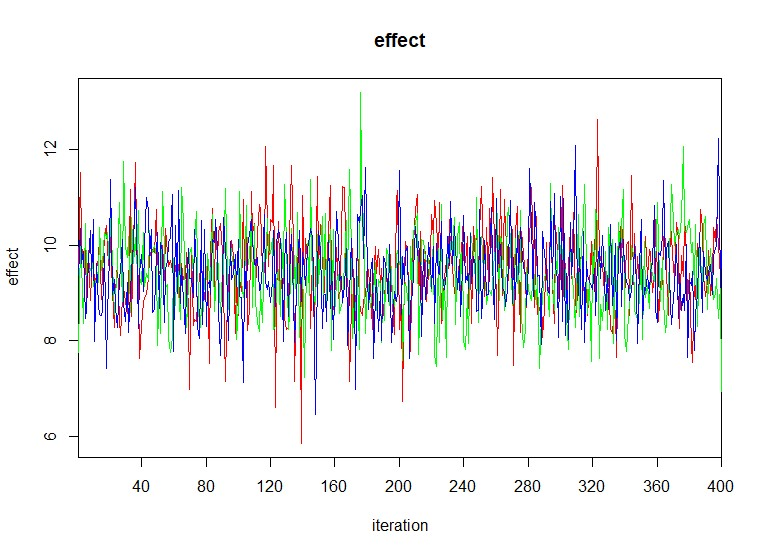
\includegraphics[keepaspectratio,alt={Trace plot showing the sampled values of a single model parameter over 400 MCMC iterations for three independent chains, shown in red, green, and blue. All three chains fluctuate randomly around a value of approximately 9 to 10 without long-term upward or downward trends. The chains overlap substantially and explore the same region of parameter space, illustrating good mixing and convergence.}]{chapters/../images/04-04.jpg}}

}

\end{figure}%

This traceplot shows that the distributions within the chains overlap
(are ``well-mixed''), and the chains are essentially stationary (do not
move up or down).

If you want a more customized traceplot, you can extract the values from
the model output. The MCMC chains are stored in the model output in
several formats. For plotting the chains, we want the values in the
\texttt{\$BUGSoutput\$sims.array}. These are the raw MCMC chains in a
3-way array that have not been permuted (i.e., the values are in the
same order as they were sampled in the MCMC process).

\subsection{Posterior distributions}\label{posterior-distributions}

Often the model outputs we are most interested in are the posterior
distributions. These represent the estimated distributions of each
parameter as supported by the data. We can learn a lot from the model
outputs printed to the R console.

For each parameter, JAGS returns and R prints the posterior mean and SD
(mu.vect and sd.vect) as well as various quantiles of the posterior
distribution. These quantiles are sample quantiles of the values from
the 3 MCMC chains.

The nature of the posterior distribution depends in large part on the
prior distribution. Most Bayesian models are formulated using
\textbf{conjugate priors}: prior distributions that, under certain
conditions, are guaranteed to result in certain posterior distributions.
In model 1, the prior distributions for parameters other than sigma were
normal. The normal is conjugate prior to itself: a normal prior will
update to a normal posterior. For sigma, we used a uniform (which does
not have a conjugate posterior) because we wanted to guarantee the
domain of the variable (\(\geq0.0001\)). It may have been more
appropriate to use an overdispersed gamma distribution or a lognormal
distribution (some textbooks recommend this for variance or SD terms).
However, in practical terms, a uniform distribution will be very similar
to a normal with very large variance within the range of the uniform.

Practically speaking, if an appropriate conjugate prior is used then the
posterior distribution will almost always be normal. Thus, the posterior
distribution can be summarized by the posterior mean and SD
(\(\mu_{post}\) and \(\sigma_{post}\)). If the normal distribution is
not appropriate for a variable (e.g., for term which must be
non-negative), then plotting its posterior distribution may be helpful.
It's worth noting that non-negative distributions can be modeled well by
the lognormal distribution, which is its own conjugate prior.

For plotting posterior distributions, we can use any of the sets of
values stored in the model output.

\begin{Shaded}
\begin{Highlighting}[]
\NormalTok{mx }\OtherTok{\textless{}{-}}\NormalTok{ mod01}\SpecialCharTok{$}\NormalTok{BUGSoutput}\SpecialCharTok{$}\NormalTok{sims.array[,,}\StringTok{"sigma"}\NormalTok{]}
\CommentTok{\# convert matrix to vector (just in case)}
\NormalTok{mx }\OtherTok{\textless{}{-}} \FunctionTok{as.numeric}\NormalTok{(mx)}
\FunctionTok{hist}\NormalTok{(mx, }\AttributeTok{main=}\StringTok{"residual SD (sigma)"}\NormalTok{)}
\end{Highlighting}
\end{Shaded}

\begin{figure}

\caption{\label{fig-posterior-histogram}Posterior distribution of the
residual standard deviation ((\sigma)) estimated by an MCMC analysis.
The histogram summarizes the posterior samples, showing the range of
plausible values for the residual standard deviation after combining the
prior information with the observed data.}

\centering{

\pandocbounded{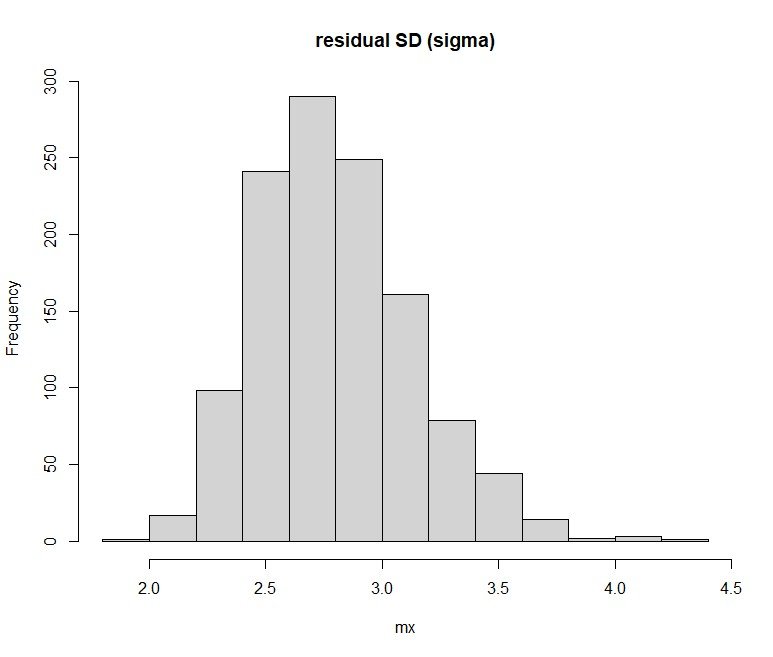
\includegraphics[keepaspectratio,alt={Histogram of posterior samples for the residual standard deviation parameter, sigma. Most posterior values lie between approximately 2.3 and 3.2, with a peak near 2.7. The distribution is unimodal and slightly right-skewed, indicating that values near 2.7 are most strongly supported by the data while larger values remain possible but progressively less probable.}]{chapters/../images/04-05.jpg}}

}

\end{figure}%

Sometimes it can be useful to plot two parameters on the same plot. This
time we'll use a kernel density plot instead of a histogram.

\begin{Shaded}
\begin{Highlighting}[]
\NormalTok{mx1 }\OtherTok{\textless{}{-}}\NormalTok{ mod01}\SpecialCharTok{$}\NormalTok{BUGSoutput}\SpecialCharTok{$}\NormalTok{sims.array[,,}\StringTok{"mu[1]"}\NormalTok{]}
\NormalTok{mx2 }\OtherTok{\textless{}{-}}\NormalTok{ mod01}\SpecialCharTok{$}\NormalTok{BUGSoutput}\SpecialCharTok{$}\NormalTok{sims.array[,,}\StringTok{"mu[2]"}\NormalTok{]}

\CommentTok{\# convert matrix to vector (just in case)}
\FunctionTok{plot}\NormalTok{(}\FunctionTok{density}\NormalTok{(mx1), }\AttributeTok{lwd=}\DecValTok{3}\NormalTok{, }\AttributeTok{xlim=}\FunctionTok{c}\NormalTok{(}\DecValTok{0}\NormalTok{, }\DecValTok{30}\NormalTok{),}
    \AttributeTok{main=}\StringTok{""}\NormalTok{)}
\FunctionTok{title}\NormalTok{(}\AttributeTok{main=}\FunctionTok{expression}\NormalTok{(Posterior}\SpecialCharTok{\textasciitilde{}}\NormalTok{densities}\SpecialCharTok{\textasciitilde{}}\NormalTok{of}\SpecialCharTok{\textasciitilde{}}\NormalTok{mu[}\DecValTok{1}\NormalTok{]}\SpecialCharTok{\textasciitilde{}}\NormalTok{and}\SpecialCharTok{\textasciitilde{}}\NormalTok{mu[}\DecValTok{2}\NormalTok{]))}
\FunctionTok{lines}\NormalTok{(}\FunctionTok{density}\NormalTok{(mx2), }\AttributeTok{lwd=}\DecValTok{3}\NormalTok{, }\AttributeTok{col=}\StringTok{"red"}\NormalTok{)}
\end{Highlighting}
\end{Shaded}

\begin{figure}

\caption{\label{fig-posterior-densities}Posterior density estimates for
two model parameters, \(\mu_1\) and \(\mu_2\). Each curve represents the
posterior probability density of a parameter estimated by MCMC. The
peaks indicate the most probable values, while the widths of the curves
reflect the uncertainty in each parameter estimate.}

\centering{

\pandocbounded{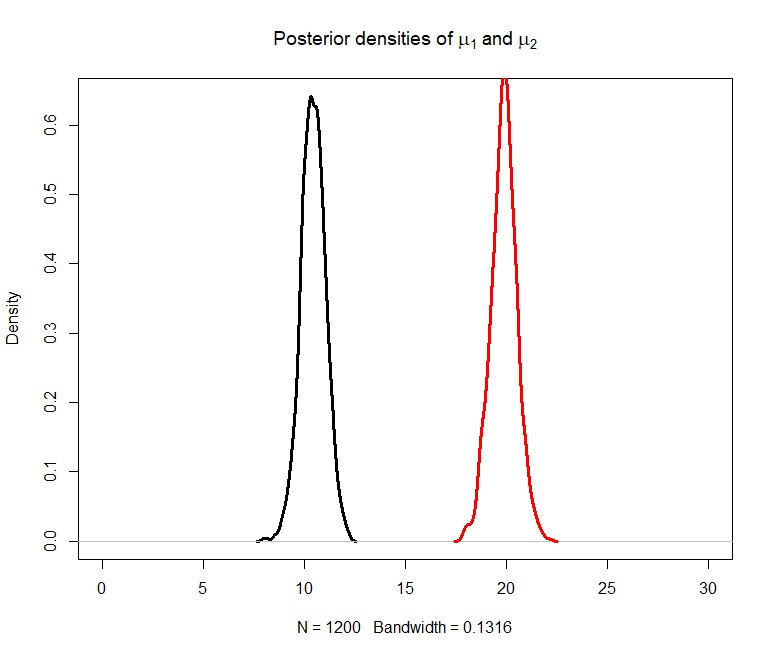
\includegraphics[keepaspectratio,alt={Kernel density plot showing the posterior distributions of two model parameters. The posterior distribution for mu-one is shown as a black curve centered near 10, and the posterior distribution for mu-two is shown as a red curve centered near 20. Both distributions are approximately symmetric and bell-shaped with relatively little overlap, indicating that the two parameter estimates are well separated and estimated with relatively high precision.}]{chapters/../images/04-06.jpg}}

}

\end{figure}%

\subsection{Predicted values}\label{predicted-values}

Finally, we can produce plots of predicted values and their credible
intervals. This isn't really useful for a t-test (where a garden variety
R boxplot works just fine), but can be extremely useful for more
complicated models (especially GLMs and mixed models). We'll explore how
to do that in the next module when we explore other linear models.

\part{Example analyses with JAGS and R}

LM, GLM, NLS, and more!

\chapter{Linear models, Bayesian style}\label{sec-linear}

This week we will continue learning the JAGS language and interface by
exploring an important class of statistical methods: the linear model.
This module includes the following common linear models:

\begin{itemize}
\tightlist
\item
  Student's \emph{t}-test
\item
  ANOVA
\item
  Linear regression (including multiple linear regression)
\item
  Analysis of covariance (ANCOVA)
\item
  \ldots and probably many more.
\end{itemize}

In one sense, these are all different ``tests'' because they test
different null hypotheses, use different test statistics, and arrive at
their \emph{p}-values differently. However, as we shall see, the
distinctions between many of the classic linear models are largely an
artifact of the different ways that \emph{p}-values are calculated. In
Bayesian inference, where P-values are not used, there is no need to
calculate a test statistic. Thus, the Bayesian modeler can look behind
the curtain and see that these are really all the same model. So, while
``what's the difference between a \emph{t}-test and ANOVA?'' is a good
exam question for an introductory (and thus frequentist) statistics
course, the question doesn't even make sense to a Bayesian. In Bayesian
inference, this question is like asking about the difference between
\(3\) and \(2+1\).

\textbf{By the end of this module you should be able to:}

\begin{enumerate}
\def\labelenumi{\arabic{enumi}.}
\tightlist
\item
  Specify common linear models in the BUGS/JAGS language.
\item
  Interpret outputs from JAGS to make inferences about biological
  systems.
\end{enumerate}

For this module you will need a recent versions of R, JAGS, and the R
packages \texttt{rjags} and \texttt{R2jags} (Plummer 2003, Plummer 2022,
R Core Team 2022, Su and Yajima 2021). This module and all code examples
were developed and tested using R version 4.2.2, JAGS 4.3.1,
\texttt{rjags} version 4-13, and \texttt{R2jags} version 0.7-1.

For this module you will need:

\begin{Shaded}
\begin{Highlighting}[]
\FunctionTok{library}\NormalTok{(rjags)}
\FunctionTok{library}\NormalTok{(R2jags)}
\end{Highlighting}
\end{Shaded}

\section{Linear models refresher}\label{linear-models-refresher}

\subsection{Enter the matrix}\label{enter-the-matrix}

\textbf{Linear models} are called linear models because they assume
\textbf{linearity}. This means that a change in some response variable
\(Y\) is described by an additive change in some predictor \(X\)
multiplied by a constant called the \textbf{slope}. The slope encodes
the change in in \(Y\) resulting from adding 1 to \(X\).

\[Y=f\left(X\right)\]

\[f\left(X+1\right)=f\left(X\right)+\beta_1\]

In practice, we also include a \emph{y}-intercept to define the value of
the function at \(X=0\).

\[f\left(0\right)=\beta_0\]

All linear models can be written very compactly in matrix notation:

\[\bf{Y}=\bf{XB}+\bf{U}\]

The boldface variables indicate that each term is really a matrix, not a
variable in the usual sense. In most biological analyses, \(\bf{Y}\),
\(\bf{B}\), and \(\bf{U}\) are column vectors, or matrices with 1
column. The matrix \(\bf{X}\) is the \textbf{design matrix}, which
contains the explanatory variables. This notation isn't very helpful for
us biologists, but it describes what the computer is doing when it fits
a model. The matrix notation above can be expanded as:

\[\left[\begin{matrix}y_1\\y_2\\\vdots\\y_n\\\end{matrix}\right]=\left[\begin{matrix}1&x_{11}&\cdots&x_{1p}\\1&x_{21}&\cdots&x_{2p}\\\vdots&\vdots&\ddots&\vdots\\1&x_{n1}&\cdots&x_{np}\\\end{matrix}\right]\left[\begin{matrix}\beta_0\\\beta_1\\\beta_2\\\vdots\\\beta_p\\\end{matrix}\right]+\left[\begin{matrix}\varepsilon_1\\\varepsilon_2\\\vdots\\\varepsilon_n\\\end{matrix}\right]\]

where \(n\) is the number of observations; \(y_1\), \(y_2\), and so on
up to \(y_n\) is a column vector of observed values of the dependent
variable (aka: response variable); \(p\) is the number of model
coefficients including the intercept; \(x_{ij}\) is the \(i\)-th value
of predictor \(j\); \(\beta_0\), \(\beta_1\), up to \(\beta_p\) is the
vector of regression coefficients; and \(\varepsilon_1\),
\(\varepsilon_2\), up to \(\varepsilon_n\) is a vector of \emph{i.i.d.}
normally distributed residuals. This matrix notation illustrates how
linear regression can be extended to models with multiple predictor
variables or even multiple response variables.

\subsection{Straight lines (somehow)}\label{straight-lines-somehow}

Another meaning of the name ``linear'' refers to the fact that the
change in the response variable \(Y\) per unit change in some predictor
variable \(X\) is a scalar (aka: constant). This means that a given
change in \(X\) will always produce the same change in \(Y\). Changing
\(X\) from 1 to 2 will have the same effect on \(Y\) as changing \(X\)
from 101 to 102, or 1,000,001 to 1,000,002, which is decidedly not the
case with nonlinear functions. In other words, the plot of \(Y\)
vs.~\(X\) will be a straight line with a constant slope. If it sounds
like I'm belaboring this point, it's because I am\ldots it's really
important!

Many models that initially appear nonlinear can nevertheless be analyzed
using linear-model methods. The important distinction is not whether the
predictors are transformed, but whether the model is linear in its
parameters.

For example, a polynomial model

\[Y = \beta_0 + \beta_1X + \beta_2X^2 + \beta_3X^3\]

is still a linear model. Although the relationship between \(Y\) and
\(X\) is curved, the quantities \(X^2\) and \(X^3\) are simply
additional predictor variables once the data are observed. The unknown
parameters \(\beta_0\), \(\beta_1\), \(\beta_2\), and \(\beta_3\) enter
the model only as coefficients.

Similarly, some nonlinear models can be transformed into linear ones.
For example, the power law

\[Y = aX^b\]

becomes

\[log\left(Y\right)=log\left(a\right)+blog\left(X\right)\]

after taking logarithms of both sides, producing a linear relationship
between \(log\left(Y\right)\) and \(log\left(X\right)\).

I think of these models as ``linear with extra steps.'' They may require
transformed variables or transformed equations, but once those
transformations are complete, they can be fit using the same machinery
as ordinary linear models.

This notion of linearity is what makes many analyses with factors
(categories or grouping variables) as predictors ``linear''. For
example, the \emph{t}-test is a linear model, but it doesn't really
describe a line on a plot of y vs.~x the way that linear regression
does. However, if you encode the factor (grouping variable) as 0s and 1s
and think about the underlying linear algebra, it becomes clear what the
difference in group means really means:

\[
\begin{bmatrix}
y_1\\
y_2\\
\vdots\\
y_n
\end{bmatrix}
=
\begin{bmatrix}
1 & x_1\\
1 & x_2\\
\vdots & \vdots\\
1 & x_n
\end{bmatrix}
\begin{bmatrix}
\beta_0\\
\beta_1
\end{bmatrix}
+
\begin{bmatrix}
\varepsilon_1\\
\varepsilon_2\\
\vdots\\
\varepsilon_n
\end{bmatrix}
\]

For any observation \(Y_i\), the expected value (without any error term)
is:

\[E\left(y_i\right)=\left(1\times\beta_0\right)+\left(x_i\times\beta_1\right)\]

For group 1, \(x_i = 0\), so the expected value is \(\beta_0\). For
group 2, \(x_i = 0\), so the \(\beta_1\) term comes into play as the
difference in means between groups 1 and 2. This is what R, SAS, and
other programs are doing internally when you analyze data with a factor
variable.

\subsection{Other details and
assumptions}\label{other-details-and-assumptions}

Linear models have some other features and assumptions that you need to
be aware of. If your data or variables violate the assumptions below,
you may need to use something other than linear models to analyze your
data.

\subsubsection{Normal residuals}\label{normal-residuals}

A model's \textbf{residuals} are the random error, or differences
between observed and predicted values. Linear models assume that
residuals follow a normal distribution. Models for data that do not have
normal residuals exist, but they are not linear models. We'll explore
those in a later module.

The assumption of normal residuals explains the last term in the linear
model equation, \(\varepsilon_i\):

\[y_i=\beta_0+\beta_1x_i+\varepsilon_i\]

In this equation, \(y_i\) is observation \(i\) of the response variable
\(y\); \(\beta_0\) is the intercept; \(\beta_1\) is the slope; \(x_i\)
is the predictor variable \(x\) for observation \(i\), and
\(\varepsilon_i\) is the residual for observation i (\(\varepsilon\) is
the Greek letter ``epsilon'' and usually stands for error or residual
terms). The residual term can be expanded like this:

\[y_i=\beta_0+\beta_1x_i+Normal\left(0,\sigma_{res}\right)\]

This expansion makes it clear that each residual \(\varepsilon_i\) comes
independently from a normal distribution with mean 0 and standard
deviation (SD) \(\sigma_{res}\). For convenience, we sometimes separate
the deterministic part and the stochastic part of the model and write
the state space form of the linear regression model:

\[y_i\sim Normal\left(\eta_i,\ \sigma_{res}\right)\]

\[\eta_i=\beta_0+\beta_1x_i\]

In this version, the symbol \$\sim \$ means ``distributed as'' and
denotes a stochastic relationship---a relationship that contains some
element of randomness. This is in contrast to a deterministic
relationship, which does not (equality, aka: identity, = is the most
famous kind of deterministic relationship).

\subsubsection{Constant variance (aka:
heteroscedasticity)}\label{constant-variance-aka-heteroscedasticity}

Linear models assume \textbf{homoscedasticity}, or constant variance.
This means that the residual variance does not depend on either \(x\) or
\(y\). This is part of the definition of a variable being independent
and identically distributed (i.i.d.). If the variance in the response
variable depends on some predictor variable, then this should be
incorporated into the model (resulting in something other than a linear
model). If the variance appears to depend on the response variable, then
there is probably an issue with the assumed response distribution (more
on this below).

The figure below shows two datasets with a linear relationship between
\(x\) and \(y\). In the left panel, the variance is the same everywhere
(homoscedastic). The right panel shows a heteroscedastic relationship
where the variance increases at larger \(x\).

\pandocbounded{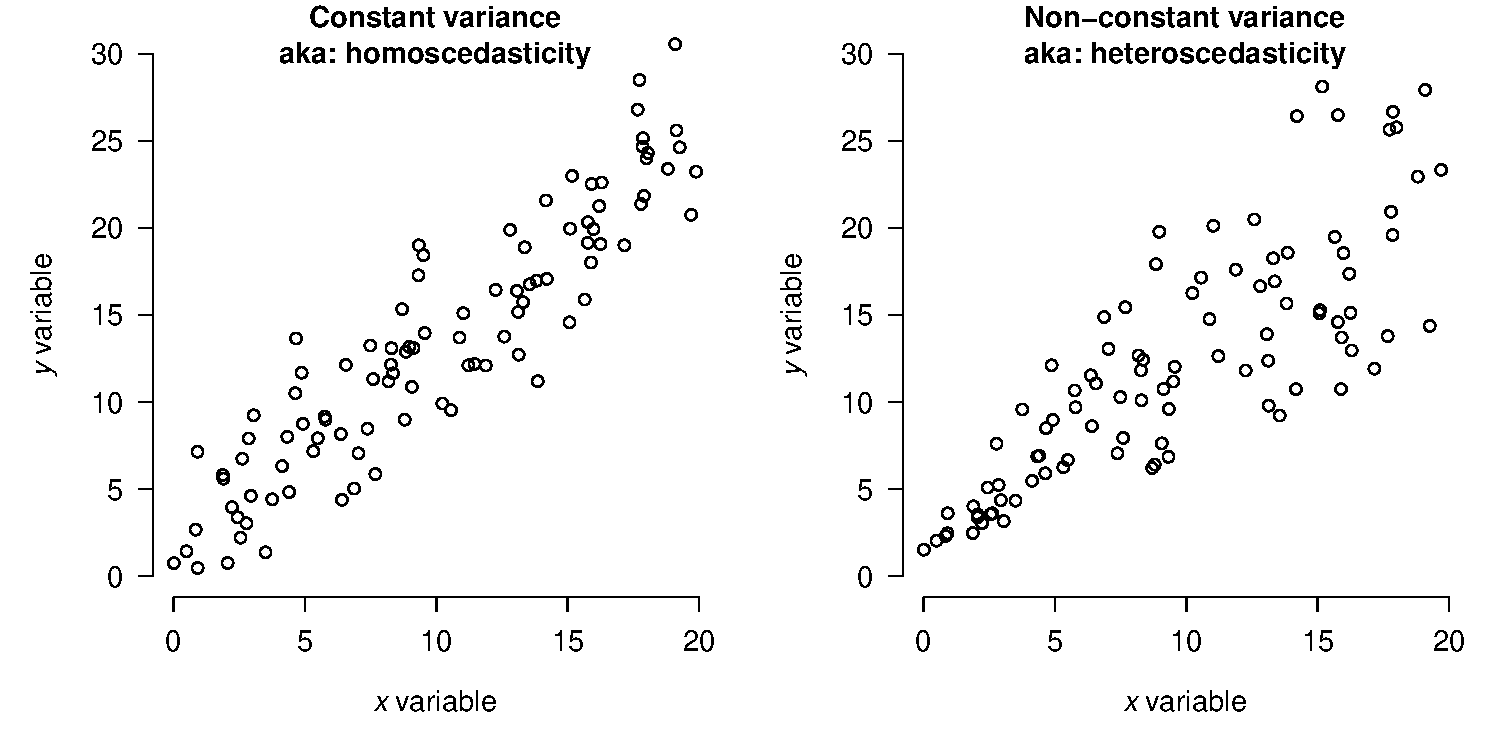
\includegraphics[keepaspectratio]{chapters/04-linear-models_files/figure-pdf/unnamed-chunk-2-1.pdf}}

The figure below shows two datasets with a categorical predictor,
suitable for a \emph{t}-test. The left panel shows a relationship with
equal variances in each group, while the right panel shows a situation
with unequal variances.

\pandocbounded{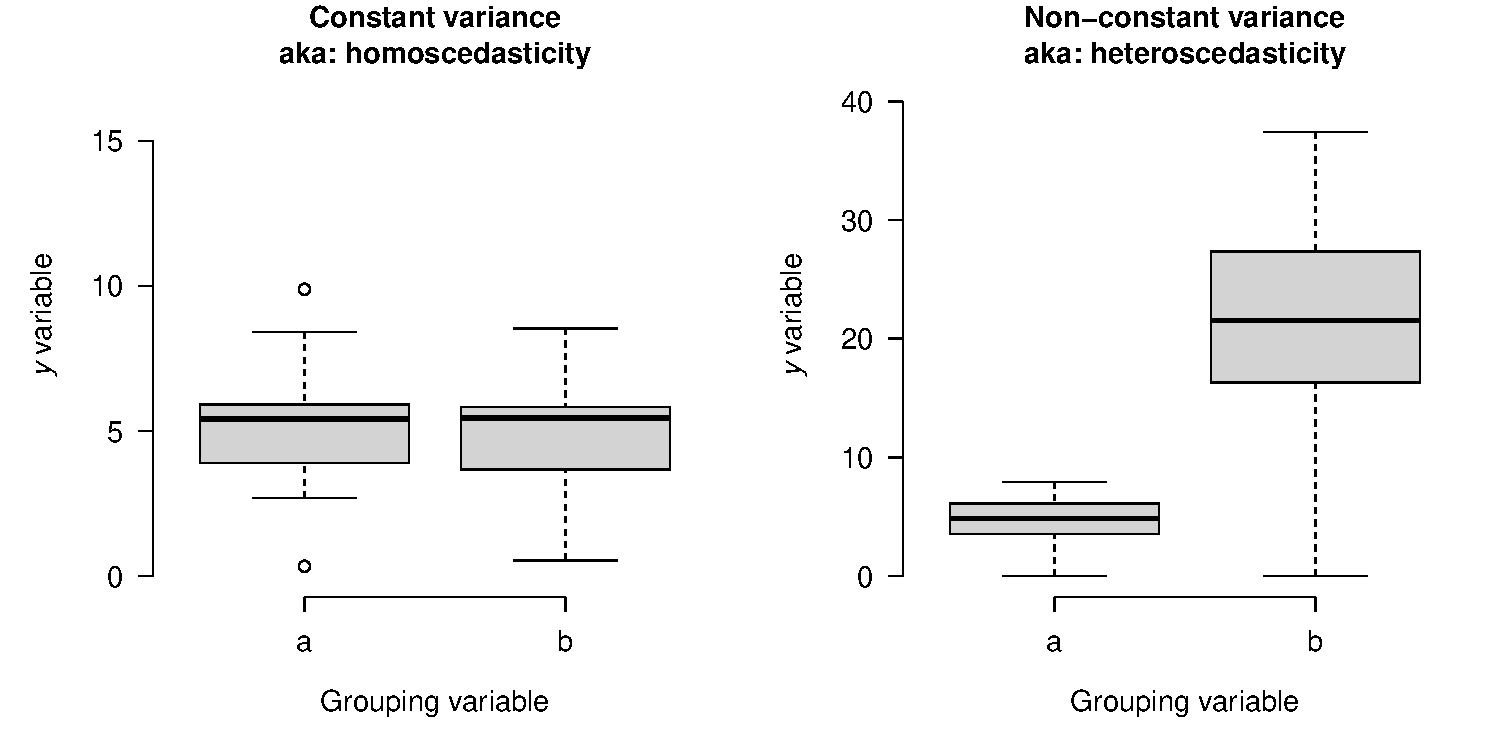
\includegraphics[keepaspectratio]{chapters/04-linear-models_files/figure-pdf/unnamed-chunk-3-1.pdf}}

\subsubsection{Fixed and independent
predictors}\label{fixed-and-independent-predictors}

Linear models assume that predictor values are precisely known
(``fixed'') and independent of each other (i.e., not autocorrelated). If
there is uncertainty in the predictor variables, this adds uncertainty
to the response values that linear models cannot account for. Simply
put, linear models have a term for uncertainty in \emph{y},
\(\sigma_{res}\), but no such term for uncertainty in \emph{x}.

\subsubsection{Independent and identically distributed errors
(i.i.d.)}\label{independent-and-identically-distributed-errors-i.i.d.}

I've mentioned this assumption before, but it bears repeating because it
is so often violated in biology. The assumption of independently and
identically distributed (i.i.d.) errors is \textbf{\emph{very}}
important. It means that the residual, or predictive error, for each
observation depends only on the parameters of the residual distribution
and not on predictor variables or other observations. When the
assumption of independence is violated, the degrees of freedom in the
analysis is artificially inflated because the number of unique pieces of
information is smaller than the nominal number of samples. In
frequentist analyses, this deflates the P-value and increases the chance
of a type I error (false positive). In Bayesian analyses, this tends to
reduce the width of the credible intervals and bias parameter estimates.
There are methods to deal with errors that are not independent, but
linear models are not among them.

\section{Comparing groups}\label{comparing-groups}

One common class of analysis is to compare the means, or central
tendencies, of groups to each other. In frequentist statistics, this is
the realm of the \emph{t}-test and ANOVA. In Bayesian statistics, they
are the same thing.

Here we have options:

\begin{itemize}
\tightlist
\item
  Compare the mean of a single set of numbers to a target value:
  \textbf{one-sample \emph{t}-test}.
\item
  Compare the means of two sets of numbers: \textbf{two-sample
  \emph{t}-test}.
\item
  Test whether the differences in paired data are different from 0 (or a
  target value): \textbf{paired \emph{t}-test}.
\item
  Compare the means of two or more sets of numbers: \textbf{analysis of
  variance (ANOVA)}.
\end{itemize}

\subsection{\texorpdfstring{Student's
\emph{t}-test}{Student's t-test}}\label{students-t-test}

We'll start with one of the most famous linear models, the Student's
\emph{t}-test. Most people have some vague idea that the \emph{t}-test
compares the means of two groups. However, the ``\emph{t}-test'' is
actually a family of tests that evaluate null hypotheses regarding
sample means. Some of the most common \emph{t}-tests are shown below:

\begin{itemize}
\tightlist
\item
  One-sample \emph{t}-test, one-tailed: Tests whether population mean of
  a single set of values is less than, or greater than, a specified
  values \(\mu_0\). Only appropriate in when differences in one
  direction only are of interest.
\item
  One-sample \emph{t}-test, two-tailed: Tests whether population mean is
  equal to some specified value \(\mu_0\) (null hypothesis) or not
  (alternative hypothesis).
\item
  Two-sample \emph{t}-test, one-tailed: Tests whether population mean of
  a one group (\(\mu_1\)) is less than, or greater than, the mean of
  another group (\(\mu_2\)). Only appropriate in when differences in one
  direction only are of interest.
\item
  Two-sample \emph{t}-test, two-tailed: Tests whether the means in two
  groups (\(\mu_1\) and \(\mu_2\)) are equal. Can also be thought of
  testing whether difference in means is equal to 0. Both equal variance
  (original) and unequal variance (Welch-Satterthwaite) versions
  exist\ldots biologists should use the unequal variance version.
\item
  Paired \emph{t}-test, one-tailed: Tests whether the mean of
  differences between paired samples
  (\({\bar{x}}_D=\frac{1}{n}\sum_{i=1}^{n}\left(x_{1,i}-x_{2,i}\right)\))
  is less than, or greater than, some specified mean difference \(D_0\).
  Only appropriate in when differences in one direction only are of
  interest.
\item
  Paired \emph{t}-test, one-tailed: Tests whether the mean of
  differences between paired samples
  (\({\bar{x}}_D=\frac{1}{n}\sum_{i=1}^{n}\left(x_{1,i}-x_{2,i}\right)\))
  is equal to 0.
\end{itemize}

These tests share a name because they revolve around the same
test-statistic, \emph{t}. The modern version of \emph{t} is the Welch's
\emph{t}, which is an improvement over the original Student's \emph{t}
that can account for unequal group sizes and group variances:

\[
t =
\frac{\bar{x}_1 - \bar{x}_2}
{\sqrt{\frac{s_1^2}{n_1} + \frac{s_2^2}{n_2}}}
\]

Then the Welch-Satterthwaite equation is used to calculate the
appropriate number of degrees of freedom (\(\nu\), ``nu''):

\[
\nu =
\frac{
\left(
\frac{s_1^2}{n_1} +
\frac{s_2^2}{n_2}
\right)^2
}{
\frac{\left(\frac{s_1^2}{n_1}\right)^2}{n_1-1}
+
\frac{\left(\frac{s_2^2}{n_2}\right)^2}{n_2-1}
}
\]

and then \emph{t} and \(\nu\) are used to calculate the \emph{p}-value.
In both equations, \({\bar{x}_i}\) is the sample mean of group \(i\),
\(S_i^2\) is the sample variance of group \(i\), and \(n_i\) is the
sample size of group \(i\). In a Bayesian analysis, we don't do any of
that.

In R, the different \emph{t}-tests are obtained with different arguments
to the function \texttt{t.test()}. Notice that the outputs have most of
the same components; the only real difference is in how the output is
interpreted. In particular, notice that the test estimates group means
and a confidence interval (CI) for either the group mean or the
difference in group means. Our Bayesian models below will also estimate
those means and differences, but they will take a more central role.

\subsubsection{\texorpdfstring{One-sample
\emph{t}-test}{One-sample t-test}}\label{sec-linear-onet}

The one sample test compares whether the mean of a set of numbers is
significantly different from some target value. By default, that target
is 0, but you can specify whatever target you like. Here are some quick
examples in R.

\begin{Shaded}
\begin{Highlighting}[]
\CommentTok{\# generate some data for demonstration}
\FunctionTok{set.seed}\NormalTok{(}\DecValTok{123}\NormalTok{)}
\NormalTok{a }\OtherTok{\textless{}{-}} \FunctionTok{rnorm}\NormalTok{(}\DecValTok{20}\NormalTok{, }\DecValTok{5}\NormalTok{, }\DecValTok{1}\NormalTok{)}

\CommentTok{\# one{-}sample test, two tails}
\DocumentationTok{\#\# Is mean of a == 0?}
\FunctionTok{t.test}\NormalTok{(a)}
\end{Highlighting}
\end{Shaded}

\begin{verbatim}

    One Sample t-test

data:  a
t = 23.64, df = 19, p-value = 1.494e-15
alternative hypothesis: true mean is not equal to 0
95 percent confidence interval:
 4.686402 5.596845
sample estimates:
mean of x 
 5.141624 
\end{verbatim}

\begin{Shaded}
\begin{Highlighting}[]
\CommentTok{\# one{-}sample test, one tail}
\DocumentationTok{\#\# Is mean of a \textgreater{} 0?}
\FunctionTok{t.test}\NormalTok{(a, }\AttributeTok{alternative=}\StringTok{"greater"}\NormalTok{)}
\end{Highlighting}
\end{Shaded}

\begin{verbatim}

    One Sample t-test

data:  a
t = 23.64, df = 19, p-value = 7.468e-16
alternative hypothesis: true mean is greater than 0
95 percent confidence interval:
 4.765547      Inf
sample estimates:
mean of x 
 5.141624 
\end{verbatim}

\begin{Shaded}
\begin{Highlighting}[]
\CommentTok{\# one{-}sample test, one tail}
\DocumentationTok{\#\# Is mean of a \textgreater{} 2?}
\FunctionTok{t.test}\NormalTok{(a, }\AttributeTok{alternative=}\StringTok{"greater"}\NormalTok{, }\AttributeTok{mu=}\DecValTok{2}\NormalTok{)}
\end{Highlighting}
\end{Shaded}

\begin{verbatim}

    One Sample t-test

data:  a
t = 14.445, df = 19, p-value = 5.334e-12
alternative hypothesis: true mean is greater than 2
95 percent confidence interval:
 4.765547      Inf
sample estimates:
mean of x 
 5.141624 
\end{verbatim}

To run a Bayesian one-sample \emph{t}-test, we need to set up our JAGS
run as outlined in Chapter~\ref{sec-jags}. Then, write this model to
text file and run JAGS. All one-sample \emph{t}-tests are the same model
in JAGS. The only difference is in how the credible interval of the mean
is interpreted.

\begin{Shaded}
\begin{Highlighting}[]
\CommentTok{\# generate data}
\FunctionTok{set.seed}\NormalTok{(}\DecValTok{123}\NormalTok{)}
\NormalTok{mu }\OtherTok{\textless{}{-}} \DecValTok{10}
\NormalTok{sigma }\OtherTok{\textless{}{-}} \DecValTok{3}
\NormalTok{n }\OtherTok{\textless{}{-}} \DecValTok{20}
\NormalTok{y }\OtherTok{\textless{}{-}} \FunctionTok{rnorm}\NormalTok{(n, mu, sigma)}

\CommentTok{\# means parameterization of one{-}sample t{-}test}
\NormalTok{mod.name }\OtherTok{\textless{}{-}} \StringTok{"jags\_ttest\_onesample.txt"}
\FunctionTok{sink}\NormalTok{(mod.name)}
\FunctionTok{cat}\NormalTok{(}\StringTok{"}
\StringTok{    model\{}
\StringTok{        \# priors}
\StringTok{        \#\# population mean}
\StringTok{        mu \textasciitilde{} dnorm(0, 0.001)        }

\StringTok{        \#\# precision and residual SD}
\StringTok{        sigma \textasciitilde{} dunif(0.0001, 10)}
\StringTok{        tau \textless{}{-} 1/(sigma\^{}2)}

\StringTok{        \# likelihood}
\StringTok{        for(i in 1:n)\{}
\StringTok{            y[i] \textasciitilde{} dnorm(mu, tau)}
\StringTok{        \}\#i}

\StringTok{    \}\#model}

\StringTok{"}\NormalTok{, }\AttributeTok{fill=}\ConstantTok{TRUE}\NormalTok{)}
\FunctionTok{sink}\NormalTok{()}

\CommentTok{\# parameters to monitor}
\NormalTok{params }\OtherTok{\textless{}{-}} \FunctionTok{c}\NormalTok{(}\StringTok{"mu"}\NormalTok{, }\StringTok{"sigma"}\NormalTok{)}

\CommentTok{\# MCMC parameters}
\NormalTok{n.iter }\OtherTok{\textless{}{-}} \FloatTok{5e4}
\NormalTok{n.burnin }\OtherTok{\textless{}{-}} \FloatTok{1e4}
\NormalTok{n.thin }\OtherTok{\textless{}{-}} \DecValTok{100}
\NormalTok{nchains }\OtherTok{\textless{}{-}} \DecValTok{3}

\CommentTok{\# function to define initial values for MCMC chains}
\NormalTok{init.fun }\OtherTok{\textless{}{-}} \ControlFlowTok{function}\NormalTok{(nc)\{}
\NormalTok{    res }\OtherTok{\textless{}{-}} \FunctionTok{vector}\NormalTok{(}\StringTok{"list"}\NormalTok{, }\AttributeTok{length=}\NormalTok{nc)}
    \ControlFlowTok{for}\NormalTok{(i }\ControlFlowTok{in} \DecValTok{1}\SpecialCharTok{:}\NormalTok{nc)\{}
\NormalTok{        res[[i]] }\OtherTok{\textless{}{-}} \FunctionTok{list}\NormalTok{(}\AttributeTok{mu=}\FunctionTok{rnorm}\NormalTok{(}\DecValTok{1}\NormalTok{, }\DecValTok{0}\NormalTok{, }\DecValTok{100}\NormalTok{),}
                         \AttributeTok{sigma=}\FunctionTok{runif}\NormalTok{(}\DecValTok{1}\NormalTok{, }\FloatTok{0.001}\NormalTok{, }\DecValTok{10}\NormalTok{))}
\NormalTok{    \}}
    \FunctionTok{return}\NormalTok{(res)}
\NormalTok{\}}
\NormalTok{inits }\OtherTok{\textless{}{-}} \FunctionTok{init.fun}\NormalTok{(nchains)}

\CommentTok{\# package data for JAGS}
\NormalTok{in.data }\OtherTok{\textless{}{-}} \FunctionTok{list}\NormalTok{(}\AttributeTok{y=}\NormalTok{y, }\AttributeTok{n=}\FunctionTok{length}\NormalTok{(y))}

\NormalTok{mod01 }\OtherTok{\textless{}{-}} \FunctionTok{jags}\NormalTok{(}\AttributeTok{data=}\NormalTok{in.data, }\AttributeTok{inits=}\NormalTok{inits,}
              \AttributeTok{parameters.to.save=}\NormalTok{params,}
              \AttributeTok{model.file=}\NormalTok{mod.name,}
              \AttributeTok{n.chains=}\NormalTok{nchains, }\AttributeTok{n.iter=}\NormalTok{n.iter,}
              \AttributeTok{n.burnin=}\NormalTok{n.burnin, }\AttributeTok{n.thin=}\NormalTok{n.thin)}\CommentTok{\#jags}
\end{Highlighting}
\end{Shaded}

\begin{verbatim}
Compiling model graph
   Resolving undeclared variables
   Allocating nodes
Graph information:
   Observed stochastic nodes: 20
   Unobserved stochastic nodes: 2
   Total graph size: 31

Initializing model
\end{verbatim}

\begin{Shaded}
\begin{Highlighting}[]
\NormalTok{mod01}
\end{Highlighting}
\end{Shaded}

\begin{verbatim}
Inference for Bugs model at "jags_ttest_onesample.txt", fit using jags,
 3 chains, each with 50000 iterations (first 10000 discarded), n.thin = 100
 n.sims = 1200 iterations saved. Running time = 1.66 secs
         mu.vect sd.vect   2.5%    25%     50%     75%   97.5%  Rhat n.eff
mu        10.449   0.712  9.006 10.002  10.457  10.904  11.828 1.002  1200
sigma      3.118   0.564  2.232  2.741   3.037   3.429   4.470 1.001  1200
deviance 100.812   2.259 98.628 99.186 100.115 101.767 107.008 1.009   540

For each parameter, n.eff is a crude measure of effective sample size,
and Rhat is the potential scale reduction factor (at convergence, Rhat=1).

DIC info (using the rule: pV = var(deviance)/2)
pV = 2.5 and DIC = 103.4
DIC is an estimate of expected predictive error (lower deviance is better).
\end{verbatim}

The most important output is the mean and 95\% CRI for \texttt{mu}. If
this interval includes the target mean \texttt{μ0}, then this is
analogous to a non-significant frequentist test and we cannot conclude
that \texttt{μ} \(\neq\) \texttt{μ0}. The 95\% CRI for \texttt{mu} is
about \texttt{{[}9.010,\ 11.846{]}}. This means, in frequentist terms,
that we can conclude that \texttt{mu} is not \textless9.010, and not
\textgreater11.846. This covers any number of one-tailed tests.
Conversely, we cannot conclude that \texttt{mu} is different from any
\texttt{μ0} found within the 95\% CRI.

\subsubsection{\texorpdfstring{Two-sample
\emph{t}-test}{Two-sample t-test}}\label{two-sample-t-test}

The two-sample \emph{t}-test is just an extension of the one-sample
\emph{t}-test. We just need to include terms for the means, sample
sizes, and variances a second group. The data that are generated below
have unequal group variances, but the model works just as well with data
that have equal variances. The unequal variances model is highly likely
to be appropriate in just about any real dataset\ldots so much so that
it is the default in R.

\begin{Shaded}
\begin{Highlighting}[]
\CommentTok{\# generate data}
\FunctionTok{set.seed}\NormalTok{(}\DecValTok{123}\NormalTok{)}
\NormalTok{mu1 }\OtherTok{\textless{}{-}} \DecValTok{10}
\NormalTok{mu2 }\OtherTok{\textless{}{-}} \DecValTok{15}
\NormalTok{sigma1 }\OtherTok{\textless{}{-}} \DecValTok{2}
\NormalTok{sigma2 }\OtherTok{\textless{}{-}} \DecValTok{1}
\NormalTok{n }\OtherTok{\textless{}{-}} \DecValTok{20}
\NormalTok{y1 }\OtherTok{\textless{}{-}} \FunctionTok{rnorm}\NormalTok{(n, mu1, sigma1)}
\NormalTok{y2 }\OtherTok{\textless{}{-}} \FunctionTok{rnorm}\NormalTok{(n, mu2, sigma2)}
\NormalTok{y }\OtherTok{\textless{}{-}} \FunctionTok{c}\NormalTok{(y1, y2)}
\NormalTok{x }\OtherTok{\textless{}{-}} \FunctionTok{rep}\NormalTok{(}\DecValTok{1}\SpecialCharTok{:}\DecValTok{2}\NormalTok{, }\AttributeTok{each=}\NormalTok{n)}

\CommentTok{\# means parameterization of two{-}sample t{-}test}
\NormalTok{mod.name }\OtherTok{\textless{}{-}} \StringTok{"jags\_ttest\_twosample.txt"}
\FunctionTok{sink}\NormalTok{(mod.name)}
\FunctionTok{cat}\NormalTok{(}\StringTok{"}
\StringTok{    model\{}
\StringTok{        \# priors}
\StringTok{        \#\# population means}
\StringTok{        for(i in 1:ngroups)\{}
\StringTok{            mu[i] \textasciitilde{} dnorm(0, 0.001)}
\StringTok{            sigma[i] \textasciitilde{} dlnorm(1, 0.25)}
\StringTok{            tau[i] \textless{}{-} 1/(sigma[i]\^{}2)}
\StringTok{        \}\#i}

\StringTok{        \# likelihood}
\StringTok{        for(i in 1:n)\{}
\StringTok{            y[i] \textasciitilde{} dnorm(mu[x[i]], tau[x[i]])}
\StringTok{        \}\#i}

\StringTok{    \}\#model}

\StringTok{"}\NormalTok{, }\AttributeTok{fill=}\ConstantTok{TRUE}\NormalTok{)}
\FunctionTok{sink}\NormalTok{()}

\CommentTok{\# parameters to monitor}
\NormalTok{params }\OtherTok{\textless{}{-}} \FunctionTok{c}\NormalTok{(}\StringTok{"mu"}\NormalTok{, }\StringTok{"sigma"}\NormalTok{)}

\CommentTok{\# MCMC parameters}
\NormalTok{n.iter }\OtherTok{\textless{}{-}} \FloatTok{5e4}
\NormalTok{n.burnin }\OtherTok{\textless{}{-}} \FloatTok{1e4}
\NormalTok{n.thin }\OtherTok{\textless{}{-}} \DecValTok{100}
\NormalTok{nchains }\OtherTok{\textless{}{-}} \DecValTok{3}

\CommentTok{\# function to define initial values for MCMC chains}
\NormalTok{init.fun }\OtherTok{\textless{}{-}} \ControlFlowTok{function}\NormalTok{(nc)\{}
\NormalTok{    res }\OtherTok{\textless{}{-}} \FunctionTok{vector}\NormalTok{(}\StringTok{"list"}\NormalTok{, }\AttributeTok{length=}\NormalTok{nc)}
    \ControlFlowTok{for}\NormalTok{(i }\ControlFlowTok{in} \DecValTok{1}\SpecialCharTok{:}\NormalTok{nc)\{}
\NormalTok{        res[[i]] }\OtherTok{\textless{}{-}} \FunctionTok{list}\NormalTok{(}\AttributeTok{mu=}\FunctionTok{rnorm}\NormalTok{(}\DecValTok{2}\NormalTok{, }\DecValTok{0}\NormalTok{, }\DecValTok{100}\NormalTok{),}
                         \AttributeTok{sigma=}\FunctionTok{runif}\NormalTok{(}\DecValTok{2}\NormalTok{, }\FloatTok{0.001}\NormalTok{, }\DecValTok{10}\NormalTok{))}
\NormalTok{    \}}
    \FunctionTok{return}\NormalTok{(res)}
\NormalTok{\}}
\NormalTok{inits }\OtherTok{\textless{}{-}} \FunctionTok{init.fun}\NormalTok{(nchains)}

\CommentTok{\# package data for JAGS}
\NormalTok{in.data }\OtherTok{\textless{}{-}} \FunctionTok{list}\NormalTok{(}\AttributeTok{y=}\NormalTok{y, }\AttributeTok{x=}\NormalTok{x, }\AttributeTok{n=}\FunctionTok{length}\NormalTok{(y), }\AttributeTok{ngroups=}\DecValTok{2}\NormalTok{)}

\NormalTok{mod02 }\OtherTok{\textless{}{-}} \FunctionTok{jags}\NormalTok{(}\AttributeTok{data=}\NormalTok{in.data, }\AttributeTok{inits=}\NormalTok{inits,}
              \AttributeTok{parameters.to.save=}\NormalTok{params,}
              \AttributeTok{model.file=}\NormalTok{mod.name,}
              \AttributeTok{n.chains=}\NormalTok{nchains, }\AttributeTok{n.iter=}\NormalTok{n.iter,}
              \AttributeTok{n.burnin=}\NormalTok{n.burnin, }\AttributeTok{n.thin=}\NormalTok{n.thin)}\CommentTok{\#jags}
\end{Highlighting}
\end{Shaded}

\begin{verbatim}
Compiling model graph
   Resolving undeclared variables
   Allocating nodes
Graph information:
   Observed stochastic nodes: 40
   Unobserved stochastic nodes: 4
   Total graph size: 95

Initializing model
\end{verbatim}

\begin{Shaded}
\begin{Highlighting}[]
\CommentTok{\# inspect results}
\NormalTok{mod02}
\end{Highlighting}
\end{Shaded}

\begin{verbatim}
Inference for Bugs model at "jags_ttest_twosample.txt", fit using jags,
 3 chains, each with 50000 iterations (first 10000 discarded), n.thin = 100
 n.sims = 1200 iterations saved. Running time = 3.59 secs
         mu.vect sd.vect    2.5%     25%     50%     75%   97.5%  Rhat n.eff
mu[1]     10.287   0.462   9.360   9.987  10.307  10.594  11.209 1.001  1200
mu[2]     14.936   0.189  14.580  14.814  14.930  15.054  15.313 1.001  1200
sigma[1]   2.021   0.337   1.487   1.767   1.979   2.230   2.790 1.001  1200
sigma[2]   0.872   0.155   0.628   0.768   0.847   0.956   1.260 1.000  1200
deviance 134.778   2.844 131.146 132.662 134.139 136.302 142.119 1.003   960

For each parameter, n.eff is a crude measure of effective sample size,
and Rhat is the potential scale reduction factor (at convergence, Rhat=1).

DIC info (using the rule: pV = var(deviance)/2)
pV = 4.0 and DIC = 138.8
DIC is an estimate of expected predictive error (lower deviance is better).
\end{verbatim}

For a standard two-sample, two-tailed \emph{t}-test, we can compare the
95\% CRI of mu{[}1{]} and mu{[}2{]}: {[}9.485, 11.223{]} and {[}14.571,
15.333{]}. These CRI do not overlap, so we can conclude that
\(\mu_1\neq\mu_2\).

For a two-sample, one-tailed test, we also compare the 95\% CRI of
\texttt{mu{[}1{]}} and \texttt{mu{[}2{]}}. The upper limit of
\texttt{mu{[}1{]}}'s CRI is less than the lower limit of the CRI for
\texttt{mu{[}2{]}}. So, for any number of one-tailed tests we could
conclude that \(\mu_1<\mu_2\).

If we are unsure whether or not a standard or Welch-Satterthwaite
(unequal variances) \emph{t}-test was warranted, we can compare the 95\%
CRI of \texttt{sigma{[}1{]}} and \texttt{sigma{[}2{]}}. These are
{[}1.512, 2.796{]} and {[}0.646, 1.222{]}. Because these CRI do not
overlap, we can conclude that groups 1 and 2 had different variances
(strictly speaking, they had different SD; you can get the variances and
their CRI by squaring the posteriors if that's what you want).

\subsubsection{\texorpdfstring{Paired
\emph{t}-tests}{Paired t-tests}}\label{paired-t-tests}

A paired \emph{t}-test is essentially a one-sample \emph{t}-test on
differences between paired samples. For example, mean body weights of
individual lab rats before and after some feeding trial.

\begin{figure}

\caption{\label{fig-paired-t-test}Comparison of two-sample and paired
\emph{t}-tests. A two-sample \emph{t}-test compares the means of two
independent groups, whereas a paired \emph{t}-test tests whether the
mean within-individual change differs from zero.}

\centering{

\pandocbounded{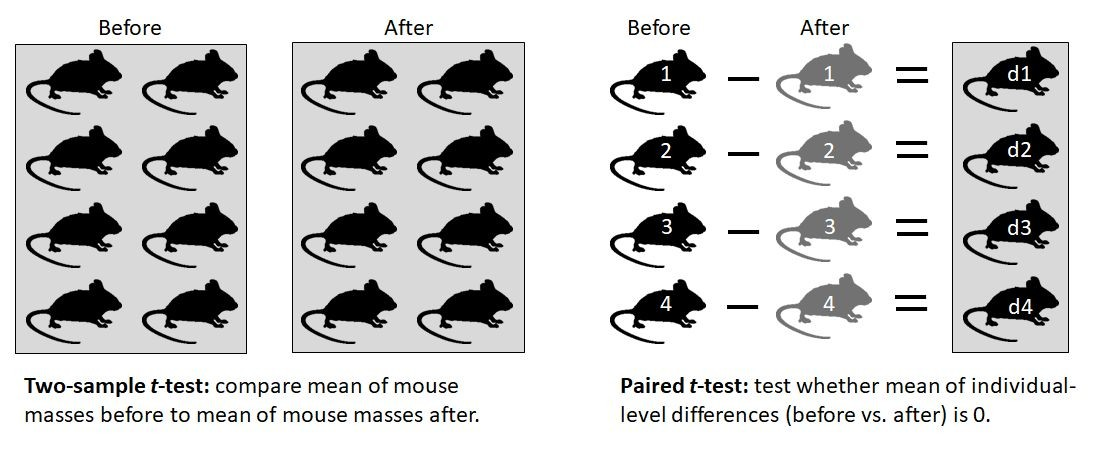
\includegraphics[keepaspectratio,alt={Diagram comparing a two-sample and a paired t-test. The left panel shows independent groups of mice measured before and after treatment, with the two-sample t-test comparing the group means. The right panel shows the same mice measured before and after treatment, with each mouse paired to itself. Individual differences (d1--d4) are calculated for each mouse, and the paired t-test tests whether the mean of these differences equals zero.}]{chapters/../images/06-01.jpg}}

}

\end{figure}%

\paragraph{Method 1: One sample test on
differences}\label{method-1-one-sample-test-on-differences}

One way to fit a paired \emph{t}-test is to calculate the differences
between the paired samples outside of JAGS, then conduct a one-sample
\emph{t}-test on the differences. Basically, calculate the differences
and feed that difference to the \texttt{jags\_ttest\_onesample} model
from Section~\ref{sec-linear-onet} as \texttt{y}.

\paragraph{Method 2: Paired test
(direct)}\label{method-2-paired-test-direct}

Alternatively, we could code the paired \emph{t}-test as its own model.
Instead of fitting group means, we can fit the mean difference directly
as \texttt{dif} and inspect its posteriors.

\begin{Shaded}
\begin{Highlighting}[]
\CommentTok{\# generate data}
\FunctionTok{set.seed}\NormalTok{(}\DecValTok{123}\NormalTok{)}
\NormalTok{n }\OtherTok{\textless{}{-}} \DecValTok{20}
\NormalTok{dif }\OtherTok{\textless{}{-}} \DecValTok{4}
\NormalTok{y1 }\OtherTok{\textless{}{-}} \FunctionTok{rnorm}\NormalTok{(n, }\DecValTok{5}\NormalTok{, }\DecValTok{1}\NormalTok{)}
\NormalTok{y2 }\OtherTok{\textless{}{-}}\NormalTok{ y1 }\SpecialCharTok{+} \FunctionTok{rnorm}\NormalTok{(n, dif, }\FloatTok{0.5}\NormalTok{)}

\CommentTok{\# means parameterization of paired t{-}test}
\NormalTok{mod.name }\OtherTok{\textless{}{-}} \StringTok{"jags\_ttest\_paired\_v1.txt"}
\FunctionTok{sink}\NormalTok{(mod.name)}
\FunctionTok{cat}\NormalTok{(}\StringTok{"}
\StringTok{    model\{}
\StringTok{        \# priors}
\StringTok{        \#\# difference in means}
\StringTok{        dif \textasciitilde{} dnorm(0, 0.001)}

\StringTok{        \#\# residual SD and precision}
\StringTok{        sigma.res \textasciitilde{} dlnorm(1, 0.25)}
\StringTok{        tau \textless{}{-} 1/(sigma.res\^{}2)}

\StringTok{        \# likelihood}
\StringTok{        for(i in 1:n)\{}
\StringTok{            y2[i] \textasciitilde{} dnorm(eta[i], tau)}
\StringTok{            eta[i] \textless{}{-} y1[i] + dif}
\StringTok{        \}\#i}

\StringTok{    \}\#model}

\StringTok{"}\NormalTok{, }\AttributeTok{fill=}\ConstantTok{TRUE}\NormalTok{)}
\FunctionTok{sink}\NormalTok{()}

\CommentTok{\# parameters to monitor}
\NormalTok{params }\OtherTok{\textless{}{-}} \FunctionTok{c}\NormalTok{(}\StringTok{"dif"}\NormalTok{, }\StringTok{"sigma.res"}\NormalTok{)}

\CommentTok{\# MCMC parameters}
\NormalTok{n.iter }\OtherTok{\textless{}{-}} \FloatTok{5e4}
\NormalTok{n.burnin }\OtherTok{\textless{}{-}} \FloatTok{1e4}
\NormalTok{n.thin }\OtherTok{\textless{}{-}} \DecValTok{100}
\NormalTok{nchains }\OtherTok{\textless{}{-}} \DecValTok{3}

\CommentTok{\# function to define initial values for MCMC chains}
\NormalTok{init.fun }\OtherTok{\textless{}{-}} \ControlFlowTok{function}\NormalTok{(nc)\{}
\NormalTok{    res }\OtherTok{\textless{}{-}} \FunctionTok{vector}\NormalTok{(}\StringTok{"list"}\NormalTok{, }\AttributeTok{length=}\NormalTok{nc)}
    \ControlFlowTok{for}\NormalTok{(i }\ControlFlowTok{in} \DecValTok{1}\SpecialCharTok{:}\NormalTok{nc)\{}
\NormalTok{        res[[i]] }\OtherTok{\textless{}{-}} \FunctionTok{list}\NormalTok{(}\AttributeTok{dif=}\FunctionTok{rnorm}\NormalTok{(}\DecValTok{1}\NormalTok{, }\DecValTok{0}\NormalTok{, }\DecValTok{100}\NormalTok{),}
                         \AttributeTok{sigma.res=}\FunctionTok{rlnorm}\NormalTok{(}\DecValTok{1}\NormalTok{, }\DecValTok{1}\NormalTok{, }\DecValTok{2}\NormalTok{))}
\NormalTok{    \}}
    \FunctionTok{return}\NormalTok{(res)}
\NormalTok{\}}
\NormalTok{inits }\OtherTok{\textless{}{-}} \FunctionTok{init.fun}\NormalTok{(nchains)}

\CommentTok{\# package data for JAGS}
\NormalTok{in.data }\OtherTok{\textless{}{-}} \FunctionTok{list}\NormalTok{(}\AttributeTok{y1=}\NormalTok{y1, }\AttributeTok{y2=}\NormalTok{y2, }\AttributeTok{n=}\NormalTok{n)}

\NormalTok{mod03 }\OtherTok{\textless{}{-}} \FunctionTok{jags}\NormalTok{(}\AttributeTok{data=}\NormalTok{in.data, }\AttributeTok{inits=}\NormalTok{inits,}
              \AttributeTok{parameters.to.save=}\NormalTok{params,}
              \AttributeTok{model.file=}\NormalTok{mod.name,}
              \AttributeTok{n.chains=}\NormalTok{nchains, }\AttributeTok{n.iter=}\NormalTok{n.iter,}
              \AttributeTok{n.burnin=}\NormalTok{n.burnin, }\AttributeTok{n.thin=}\NormalTok{n.thin)}\CommentTok{\#jags}
\end{Highlighting}
\end{Shaded}

\begin{verbatim}
Compiling model graph
   Resolving undeclared variables
   Allocating nodes
Graph information:
   Observed stochastic nodes: 20
   Unobserved stochastic nodes: 2
   Total graph size: 70

Initializing model
\end{verbatim}

\begin{Shaded}
\begin{Highlighting}[]
\NormalTok{mod03}
\end{Highlighting}
\end{Shaded}

\begin{verbatim}
Inference for Bugs model at "jags_ttest_paired_v1.txt", fit using jags,
 3 chains, each with 50000 iterations (first 10000 discarded), n.thin = 100
 n.sims = 1200 iterations saved. Running time = 1.69 secs
          mu.vect sd.vect   2.5%    25%   50%    75%  97.5%  Rhat n.eff
dif         3.972   0.096  3.776  3.908  3.97  4.032  4.160 1.000  1200
sigma.res   0.441   0.077  0.319  0.385  0.43  0.485  0.610 1.000  1200
deviance   22.653   2.079 20.614 21.162 22.03 23.364 28.083 1.001  1200

For each parameter, n.eff is a crude measure of effective sample size,
and Rhat is the potential scale reduction factor (at convergence, Rhat=1).

DIC info (using the rule: pV = var(deviance)/2)
pV = 2.2 and DIC = 24.8
DIC is an estimate of expected predictive error (lower deviance is better).
\end{verbatim}

The result is spot-on what is estimated by the base R \texttt{t.test()}
function:

\begin{Shaded}
\begin{Highlighting}[]
\FunctionTok{t.test}\NormalTok{(y1, y2, }\AttributeTok{paired=}\ConstantTok{TRUE}\NormalTok{)}
\end{Highlighting}
\end{Shaded}

\begin{verbatim}

    Paired t-test

data:  y1 and y2
t = -42.832, df = 19, p-value < 2.2e-16
alternative hypothesis: true mean difference is not equal to 0
95 percent confidence interval:
 -4.168583 -3.780160
sample estimates:
mean difference 
      -3.974371 
\end{verbatim}

\subsection{Analysis of variance
(ANOVA)}\label{analysis-of-variance-anova}

The analysis of variance (ANOVA) is another case of the linear model. It
is usually used to compare the means of 3 or more groups. In this way it
can be thought of as an extension of the \emph{t}-test from 2 groups to
\textgreater2, but this is incorrect from a frequentist perspective
because of how differently the \emph{t}-test and ANOVA arrive at a
\emph{p}-value. It's better to think of the frequentist \emph{t}-test
and ANOVA as cousins. Frequentist ANOVA assesses statistical
significance using the statistic \emph{F}, which is related to the
amount of variance associated with different sources of variance,
relative to the number of degrees of freedom. This is different from t,
which is a difference in means scaled by variances and sample sizes,
\emph{F}. Either way, \emph{t} and \emph{F} (and all test statistics)
are just contrivances to obtain a \emph{p}-value. In Bayesian
statistics, we don't need that.

Consider this model:

\[y_i\sim Normal\left(\mu_{x_i},\ \sigma_{res.}\right)\]

If \(\mu_{x_i}\) is the mean for the group defined by xi, then what is
this model saying? It's saying that the value of y for observation
\emph{i} is drawn from a normal distribution with a mean that depends on
group of observation \emph{i}, and some residual variation
\(\sigma_{res.}\). This single model covers a lot of situations:

\begin{itemize}
\tightlist
\item
  If the number of groups is 1, then this is a one-sample \emph{t}-test
\item
  If the number of groups is 2, then this is a two-sample \emph{t}-test.
  Or, a one-way ANOVA with two factor levels.
\item
  If the number of groups is 3, then this is a one-way ANOVA with three
  factor levels.
\item
  If the number of groups is 1, but the values represented paired
  differences, then this is a paired \emph{t}-test.
\end{itemize}

All four of these methods, which have different names and different
fitting methods in frequentist statistics, are the same model for a
Bayesian and can be fit with the same code in JAGS. This kind of
generalization is one of the greatest things about Bayesian inference
and MCMC model fitting. By getting away from a hyper-fixation on test
statistics and \emph{p}-values, we can take a step back and think about
what our models really mean.

\subsubsection{ANOVA basics}\label{anova-basics}

In a typical frequentist ANOVA, one first conducts the omnibus test,
which assesses whether any of the group means differ from each other.
Then, a post-hoc test is performed to check which groups differ from
each other. The code below illustrates this process in R using the
built-in \texttt{iris} dataset.

\begin{Shaded}
\begin{Highlighting}[]
\CommentTok{\# fit the model for anova()}
\NormalTok{mod1 }\OtherTok{\textless{}{-}} \FunctionTok{aov}\NormalTok{(Petal.Length}\SpecialCharTok{\textasciitilde{}}\NormalTok{Species, }\AttributeTok{data=}\NormalTok{iris)}

\CommentTok{\# omnibus test to get ANOVA table:}
\FunctionTok{summary}\NormalTok{(mod1)}
\end{Highlighting}
\end{Shaded}

\begin{verbatim}
             Df Sum Sq Mean Sq F value Pr(>F)    
Species       2  437.1  218.55    1180 <2e-16 ***
Residuals   147   27.2    0.19                   
---
Signif. codes:  0 '***' 0.001 '**' 0.01 '*' 0.05 '.' 0.1 ' ' 1
\end{verbatim}

This is the omnibus test result, or ``ANOVA table''.The ANOVA table
shows us that the factor species uses 2 degrees of freedom (Df or d.f.)
to account for 437.10 of the squared errors; the residuals use 147 d.f.
to account for 27.22 of the squared errors. The ratio of the mean
squared error per d.f. associated with each source, 218.551 / 0.185 =
1180.2, is the test statistic F. The is used to calculate the
\emph{p}-value. We can also see that about 94.1\% of variation (437.10 /
(437.10+27.22)) is associated with species.

However, all the \emph{p}-value in the omnibus test tells us is that the
means of at least one pair of species differ. To find out which pair or
pairs, we need to use a post-hoc test. My favorite is the Tukey's honest
significant difference (HSD) test because it automatically adjusts for
multiple comparisons.

\begin{Shaded}
\begin{Highlighting}[]
\CommentTok{\# post{-}hoc test:}
\FunctionTok{TukeyHSD}\NormalTok{(mod1)}
\end{Highlighting}
\end{Shaded}

\begin{verbatim}
  Tukey multiple comparisons of means
    95% family-wise confidence level

Fit: aov(formula = Petal.Length ~ Species, data = iris)

$Species
                      diff     lwr     upr p adj
versicolor-setosa    2.798 2.59422 3.00178     0
virginica-setosa     4.090 3.88622 4.29378     0
virginica-versicolor 1.292 1.08822 1.49578     0
\end{verbatim}

This result shows us that all of the species differ from each other. We
can see this because all of the \emph{p}-values (\texttt{p\ adj}) for
the pairwise comparisons are \textless0.05 (they are printed by R as 0,
but are really just approximated to very tiny value). We can also see
this because the 95\% CI for the pairwise differences do not include 0.
For example, the difference in means for species \texttt{versicolor} and
\texttt{setosa} is 2.798, with 95\% CI = {[}2.59, 3.00{]}. The value
\texttt{diff} is literally the mean of \texttt{versicolor} minus the
mean of \texttt{setosa}, as printed on the left of the table.

This is a lot of work. Remember, most of the testing and interpretation
in this ANOVA was really just steps taken to get a \emph{p}-value. By
using a means parameterization in JAGS, we can get everything in one
step in JAGS.

\subsubsection{One-way ANOVA in JAGS}\label{one-way-anova-in-jags}

The previous example with the iris data is an example of one-way ANOVA.
The ``-way'' part just defines how many explanatory factors there are.
In the next section we'll try ``two-way'' ANOVA, which has 2 factors.

A basic one-way ANOVA model can be fitted in JAGS using essentially the
same code as for the two-sample \emph{t}-test (see above). All that we
have to adjust are some of the inputs, including \texttt{ngroups} (which
was 2 for the \emph{t}-test, but can be any positive integer in ANOVA).
We'll use the \texttt{iris} dataset as in the previous example

\begin{Shaded}
\begin{Highlighting}[]
\NormalTok{mod.name }\OtherTok{\textless{}{-}} \StringTok{"jags\_anova\_oneway.txt"}
\FunctionTok{sink}\NormalTok{(mod.name)}
\FunctionTok{cat}\NormalTok{(}\StringTok{"}
\StringTok{    model\{}
\StringTok{        \# priors}
\StringTok{        \#\# population means}
\StringTok{        for(i in 1:ngroups)\{}
\StringTok{            mu[i] \textasciitilde{} dnorm(0, 0.001)}
\StringTok{            sigma[i] \textasciitilde{} dlnorm(1, 0.25)}
\StringTok{            tau[i] \textless{}{-} 1/(sigma[i]\^{}2)}
\StringTok{        \}\#i}

\StringTok{        \# likelihood}
\StringTok{        for(i in 1:n)\{}
\StringTok{            y[i] \textasciitilde{} dnorm(mu[x[i]], tau[x[i]])}
\StringTok{        \}\#i}

\StringTok{    \}\#model}

\StringTok{"}\NormalTok{, }\AttributeTok{fill=}\ConstantTok{TRUE}\NormalTok{)}
\FunctionTok{sink}\NormalTok{()}

\CommentTok{\# parameters to monitor}
\NormalTok{params }\OtherTok{\textless{}{-}} \FunctionTok{c}\NormalTok{(}\StringTok{"mu"}\NormalTok{, }\StringTok{"sigma"}\NormalTok{)}

\CommentTok{\# MCMC parameters}
\NormalTok{n.iter }\OtherTok{\textless{}{-}} \FloatTok{5e4}
\NormalTok{n.burnin }\OtherTok{\textless{}{-}} \FloatTok{1e4}
\NormalTok{n.thin }\OtherTok{\textless{}{-}} \DecValTok{100}
\NormalTok{nchains }\OtherTok{\textless{}{-}} \DecValTok{3}

\CommentTok{\# function to define initial values for MCMC chains}
\NormalTok{init.fun }\OtherTok{\textless{}{-}} \ControlFlowTok{function}\NormalTok{(nc, }\AttributeTok{ngroups=}\DecValTok{3}\NormalTok{)\{}
\NormalTok{    res }\OtherTok{\textless{}{-}} \FunctionTok{vector}\NormalTok{(}\StringTok{"list"}\NormalTok{, }\AttributeTok{length=}\NormalTok{nc)}
    \ControlFlowTok{for}\NormalTok{(i }\ControlFlowTok{in} \DecValTok{1}\SpecialCharTok{:}\NormalTok{nc)\{}
\NormalTok{        res[[i]] }\OtherTok{\textless{}{-}} \FunctionTok{list}\NormalTok{(}\AttributeTok{mu=}\FunctionTok{rnorm}\NormalTok{(ngroups, }\DecValTok{0}\NormalTok{, }\DecValTok{100}\NormalTok{),}
                         \AttributeTok{sigma=}\FunctionTok{rlnorm}\NormalTok{(ngroups, }\DecValTok{1}\NormalTok{, }\DecValTok{2}\NormalTok{))}
\NormalTok{    \}}
    \FunctionTok{return}\NormalTok{(res)}
\NormalTok{\}}
\NormalTok{inits }\OtherTok{\textless{}{-}} \FunctionTok{init.fun}\NormalTok{(nchains, }\DecValTok{3}\NormalTok{)}

\CommentTok{\# package data for JAGS}
\NormalTok{xfac }\OtherTok{\textless{}{-}} \FunctionTok{match}\NormalTok{(iris}\SpecialCharTok{$}\NormalTok{Species, }\FunctionTok{sort}\NormalTok{(}\FunctionTok{unique}\NormalTok{(iris}\SpecialCharTok{$}\NormalTok{Species)))}
\NormalTok{ngroups }\OtherTok{\textless{}{-}} \FunctionTok{max}\NormalTok{(xfac)}
\NormalTok{in.data }\OtherTok{\textless{}{-}} \FunctionTok{list}\NormalTok{(}\AttributeTok{y=}\NormalTok{iris}\SpecialCharTok{$}\NormalTok{Petal.Length,}
    \AttributeTok{x=}\NormalTok{xfac, }\AttributeTok{n=}\FunctionTok{nrow}\NormalTok{(iris), }\AttributeTok{ngroups=}\NormalTok{ngroups)}

\NormalTok{mod05 }\OtherTok{\textless{}{-}} \FunctionTok{jags}\NormalTok{(}\AttributeTok{data=}\NormalTok{in.data, }\AttributeTok{inits=}\NormalTok{inits,}
              \AttributeTok{parameters.to.save=}\NormalTok{params,}
              \AttributeTok{model.file=}\NormalTok{mod.name,}
              \AttributeTok{n.chains=}\NormalTok{nchains, }\AttributeTok{n.iter=}\NormalTok{n.iter,}
              \AttributeTok{n.burnin=}\NormalTok{n.burnin, }\AttributeTok{n.thin=}\NormalTok{n.thin)}\CommentTok{\#jags}
\end{Highlighting}
\end{Shaded}

\begin{verbatim}
Compiling model graph
   Resolving undeclared variables
   Allocating nodes
Graph information:
   Observed stochastic nodes: 150
   Unobserved stochastic nodes: 6
   Total graph size: 319

Initializing model
\end{verbatim}

\begin{Shaded}
\begin{Highlighting}[]
\NormalTok{mod05}
\end{Highlighting}
\end{Shaded}

\begin{verbatim}
Inference for Bugs model at "jags_anova_oneway.txt", fit using jags,
 3 chains, each with 50000 iterations (first 10000 discarded), n.thin = 100
 n.sims = 1200 iterations saved. Running time = 12.11 secs
         mu.vect sd.vect    2.5%     25%     50%     75%   97.5%  Rhat n.eff
mu[1]      1.462   0.025   1.412   1.445   1.462   1.479   1.509 1.002  1100
mu[2]      4.257   0.065   4.133   4.211   4.256   4.301   4.382 1.002  1200
mu[3]      5.552   0.081   5.391   5.498   5.554   5.605   5.719 1.012   160
sigma[1]   0.178   0.018   0.147   0.166   0.177   0.189   0.217 1.000  1200
sigma[2]   0.481   0.049   0.397   0.447   0.476   0.511   0.583 1.003   570
sigma[3]   0.560   0.055   0.465   0.522   0.556   0.595   0.678 1.000  1200
deviance 118.592   3.441 113.758 116.068 117.958 120.434 126.862 1.000  1200

For each parameter, n.eff is a crude measure of effective sample size,
and Rhat is the potential scale reduction factor (at convergence, Rhat=1).

DIC info (using the rule: pV = var(deviance)/2)
pV = 5.9 and DIC = 124.5
DIC is an estimate of expected predictive error (lower deviance is better).
\end{verbatim}

Unlike the frequentist ANOVA we performed in R, there is no need for
post-hoc test in the Bayesian version of the model. Instead of
performing a separate test, we can compare the 95\% CRI of the group
means directly. For example, species 1 and 2 have different petal
lengths because their 95\% CRI don't overlap.

\subsubsection{Two-way ANOVA in JAGS}\label{two-way-anova-in-jags}

In a two-way ANOVA, the variation is partitioned among two potentially
explanatory factors---i.e., the variation is split in two ways. There is
also three-way ANOVA, four-way ANOVA, and so on. We'll focus on two-way
ANOVA because the code is relatively simple to generalize to other
situations.

In base R, we can add more factors to the model with the plus sign
\texttt{+}.

\begin{Shaded}
\begin{Highlighting}[]
\CommentTok{\# make a spare copy of iris, and add a variable for color}
\CommentTok{\# (which doesn\textquotesingle{}t explain anything)}
\NormalTok{iris2 }\OtherTok{\textless{}{-}}\NormalTok{ iris}
\NormalTok{iris2}\SpecialCharTok{$}\NormalTok{color }\OtherTok{\textless{}{-}} \FunctionTok{c}\NormalTok{(}\StringTok{"red"}\NormalTok{, }\StringTok{"white"}\NormalTok{)}

\CommentTok{\# fit the two{-}way anova}
\NormalTok{mod2 }\OtherTok{\textless{}{-}} \FunctionTok{aov}\NormalTok{(Petal.Length}\SpecialCharTok{\textasciitilde{}}\NormalTok{Species}\SpecialCharTok{+}\NormalTok{color,}
            \AttributeTok{data=}\NormalTok{iris2)}
\FunctionTok{anova}\NormalTok{(mod2)}
\end{Highlighting}
\end{Shaded}

\begin{verbatim}
Analysis of Variance Table

Response: Petal.Length
           Df Sum Sq Mean Sq   F value Pr(>F)    
Species     2 437.10 218.551 1174.2292 <2e-16 ***
color       1   0.05   0.049    0.2611 0.6101    
Residuals 146  27.17   0.186                     
---
Signif. codes:  0 '***' 0.001 '**' 0.01 '*' 0.05 '.' 0.1 ' ' 1
\end{verbatim}

\begin{Shaded}
\begin{Highlighting}[]
\FunctionTok{TukeyHSD}\NormalTok{(mod2)}
\end{Highlighting}
\end{Shaded}

\begin{verbatim}
  Tukey multiple comparisons of means
    95% family-wise confidence level

Fit: aov(formula = Petal.Length ~ Species + color, data = iris2)

$Species
                      diff      lwr      upr p adj
versicolor-setosa    2.798 2.593692 3.002308     0
virginica-setosa     4.090 3.885692 4.294308     0
virginica-versicolor 1.292 1.087692 1.496308     0

$color
            diff        lwr       upr     p adj
white-red -0.036 -0.1752347 0.1032347 0.6101255
\end{verbatim}

In JAGS, we can get everything in one step. We'll fit the effects
parameterization because it's easier to define independent effects of
species and color this way. Notice that we have to play a little trick
in the priors for beta1 and beta2. Technically, the ``effect'' for the
baseline level of a factor should be 0. However, this is not allowed in
JAGS because it would have required having some elements of the vectors
beta1 and beta2 being deterministic (i.e.,
\texttt{beta1{[}1{]}\ \textless{}-\ 0}), while having other elements of
those vectors be stochastic (e.g.,
\texttt{beta1{[}2{]}\ \textasciitilde{}\ dnorm(0,\ 0.001)}). This
provokes the error message,
``\texttt{Cannot\ set\ value\ of\ non-variable\ node}''.

The solution is to define the prior for the baseline levels to have
essentially 0 variance about the true value of 0. We used a normal with
\(\mu=0\) and \(\sigma^2=0.000000001\). Another way to look at this is
that we place a very strong prior on this parameter, so strong that no
amount of data would be sufficient to update it.

\begin{Shaded}
\begin{Highlighting}[]
\NormalTok{iris2 }\OtherTok{\textless{}{-}}\NormalTok{ iris}
\NormalTok{iris2}\SpecialCharTok{$}\NormalTok{color }\OtherTok{\textless{}{-}} \FunctionTok{c}\NormalTok{(}\StringTok{"red"}\NormalTok{, }\StringTok{"white"}\NormalTok{)}

\CommentTok{\# effects parameterization of two{-}way ANOVA}
\CommentTok{\# without interaction (main effects)}
\NormalTok{mod.name }\OtherTok{\textless{}{-}} \StringTok{"jags\_anova2way\_main.txt"}
\FunctionTok{sink}\NormalTok{(mod.name)}
\FunctionTok{cat}\NormalTok{(}\StringTok{"}
\StringTok{    model\{}
\StringTok{        \# priors}
\StringTok{        \#\# intercept}
\StringTok{        beta0 \textasciitilde{} dnorm(0, 0.001)}

\StringTok{        \#\# effects of factor 1}
\StringTok{        beta1[1] \textasciitilde{} dnorm(0, 1e9) \# set first level to 0}
\StringTok{        beta1[2] \textasciitilde{} dnorm(0, 0.001)}
\StringTok{        beta1[3] \textasciitilde{} dnorm(0, 0.001)}

\StringTok{        \#\# effects of factor 2}
\StringTok{        beta2[1] \textasciitilde{} dnorm(0, 1e9) \# set first level to 0}
\StringTok{        beta2[2] \textasciitilde{} dnorm(0, 0.001)}

\StringTok{        \#\# residual SD and precision}
\StringTok{        sigma \textasciitilde{} dlnorm(1, 0.25)}
\StringTok{        tau \textless{}{-} 1 / (sigma\^{}2)}

\StringTok{        \# likelihood}
\StringTok{        for(i in 1:n)\{}
\StringTok{            y[i] \textasciitilde{} dnorm(eta[i], tau)}
\StringTok{            eta[i] \textless{}{-} beta0 + beta1[fac1[i]] + beta2[fac2[i]]}
\StringTok{        \}\#i}

\StringTok{    \}\#model}

\StringTok{"}\NormalTok{, }\AttributeTok{fill=}\ConstantTok{TRUE}\NormalTok{)}
\FunctionTok{sink}\NormalTok{()}

\CommentTok{\# parameters to monitor}
\NormalTok{params }\OtherTok{\textless{}{-}} \FunctionTok{c}\NormalTok{(}\StringTok{"beta0"}\NormalTok{, }\StringTok{"beta1"}\NormalTok{, }\StringTok{"beta2"}\NormalTok{, }\StringTok{"sigma"}\NormalTok{)}

\CommentTok{\# MCMC parameters}
\NormalTok{n.iter }\OtherTok{\textless{}{-}} \FloatTok{5e4}
\NormalTok{n.burnin }\OtherTok{\textless{}{-}} \FloatTok{1e4}
\NormalTok{n.thin }\OtherTok{\textless{}{-}} \DecValTok{100}
\NormalTok{nchains }\OtherTok{\textless{}{-}} \DecValTok{3}

\CommentTok{\# reformat data for JAGS}
\NormalTok{fac1 }\OtherTok{\textless{}{-}} \FunctionTok{match}\NormalTok{(iris2}\SpecialCharTok{$}\NormalTok{Species, }\FunctionTok{sort}\NormalTok{(}\FunctionTok{unique}\NormalTok{(iris2}\SpecialCharTok{$}\NormalTok{Species)))}
\NormalTok{nfac1 }\OtherTok{\textless{}{-}} \FunctionTok{max}\NormalTok{(fac1)}
\NormalTok{fac2 }\OtherTok{\textless{}{-}} \FunctionTok{match}\NormalTok{(iris2}\SpecialCharTok{$}\NormalTok{color, }\FunctionTok{sort}\NormalTok{(}\FunctionTok{unique}\NormalTok{(iris2}\SpecialCharTok{$}\NormalTok{color)))}
\NormalTok{nfac2 }\OtherTok{\textless{}{-}} \FunctionTok{max}\NormalTok{(fac2)}

\CommentTok{\# package data for JAGS}
\NormalTok{in.data }\OtherTok{\textless{}{-}} \FunctionTok{list}\NormalTok{(}\AttributeTok{y=}\NormalTok{iris2}\SpecialCharTok{$}\NormalTok{Petal.Length,}
    \AttributeTok{n=}\FunctionTok{nrow}\NormalTok{(iris2),}
    \AttributeTok{fac1=}\NormalTok{fac1, }\AttributeTok{fac2=}\NormalTok{fac2)}

\CommentTok{\# function to define initial values for MCMC chains}
\NormalTok{init.fun }\OtherTok{\textless{}{-}} \ControlFlowTok{function}\NormalTok{(nc)\{}
\NormalTok{    res }\OtherTok{\textless{}{-}} \FunctionTok{vector}\NormalTok{(}\StringTok{"list"}\NormalTok{, }\AttributeTok{length=}\NormalTok{nc)}
    \ControlFlowTok{for}\NormalTok{(i }\ControlFlowTok{in} \DecValTok{1}\SpecialCharTok{:}\NormalTok{nc)\{}
\NormalTok{        res[[i]] }\OtherTok{\textless{}{-}} \FunctionTok{list}\NormalTok{(}\AttributeTok{beta0=}\FunctionTok{rnorm}\NormalTok{(}\DecValTok{1}\NormalTok{, }\DecValTok{0}\NormalTok{, }\DecValTok{100}\NormalTok{),}
                         \AttributeTok{beta1=}\FunctionTok{c}\NormalTok{(}\DecValTok{0}\NormalTok{, }\FunctionTok{rnorm}\NormalTok{(nfac1}\DecValTok{{-}1}\NormalTok{, }\DecValTok{0}\NormalTok{, }\DecValTok{100}\NormalTok{)),}
                         \AttributeTok{beta2=}\FunctionTok{c}\NormalTok{(}\DecValTok{0}\NormalTok{, }\FunctionTok{rnorm}\NormalTok{(nfac2}\DecValTok{{-}1}\NormalTok{, }\DecValTok{0}\NormalTok{, }\DecValTok{100}\NormalTok{)),}
                         \AttributeTok{sigma=}\FunctionTok{rlnorm}\NormalTok{(}\DecValTok{1}\NormalTok{, }\DecValTok{1}\NormalTok{, }\DecValTok{2}\NormalTok{))}
\NormalTok{    \}}
    \FunctionTok{return}\NormalTok{(res)}
\NormalTok{\}}
\NormalTok{inits }\OtherTok{\textless{}{-}} \FunctionTok{init.fun}\NormalTok{(nchains)}

\CommentTok{\# fit model}
\NormalTok{mod06 }\OtherTok{\textless{}{-}} \FunctionTok{jags}\NormalTok{(}\AttributeTok{data=}\NormalTok{in.data, }\AttributeTok{inits=}\NormalTok{inits,}
              \AttributeTok{parameters.to.save=}\NormalTok{params,}
              \AttributeTok{model.file=}\NormalTok{mod.name,}
              \AttributeTok{n.chains=}\NormalTok{nchains, }\AttributeTok{n.iter=}\NormalTok{n.iter,}
              \AttributeTok{n.burnin=}\NormalTok{n.burnin, }\AttributeTok{n.thin=}\NormalTok{n.thin)}\CommentTok{\#jags}
\end{Highlighting}
\end{Shaded}

\begin{verbatim}
Compiling model graph
   Resolving undeclared variables
   Allocating nodes
Graph information:
   Observed stochastic nodes: 150
   Unobserved stochastic nodes: 7
   Total graph size: 472

Initializing model
\end{verbatim}

\begin{Shaded}
\begin{Highlighting}[]
\NormalTok{mod06}
\end{Highlighting}
\end{Shaded}

\begin{verbatim}
Inference for Bugs model at "jags_anova2way_main.txt", fit using jags,
 3 chains, each with 50000 iterations (first 10000 discarded), n.thin = 100
 n.sims = 1200 iterations saved. Running time = 14.72 secs
         mu.vect sd.vect    2.5%     25%     50%     75%   97.5%  Rhat n.eff
beta0      1.481   0.072   1.339   1.433   1.479   1.527   1.632 1.002   750
beta1[1]   0.000   0.000   0.000   0.000   0.000   0.000   0.000 1.000     1
beta1[2]   2.799   0.088   2.633   2.740   2.797   2.857   2.968 1.004   510
beta1[3]   4.089   0.091   3.914   4.028   4.088   4.150   4.266 1.002  1100
beta2[1]   0.000   0.000   0.000   0.000   0.000   0.000   0.000 1.000     1
beta2[2]  -0.037   0.069  -0.173  -0.081  -0.040   0.008   0.100 1.001  1200
sigma      0.436   0.026   0.389   0.418   0.434   0.452   0.489 1.000  1200
deviance 174.594   3.300 170.318 172.208 173.877 176.355 182.549 1.001  1200

For each parameter, n.eff is a crude measure of effective sample size,
and Rhat is the potential scale reduction factor (at convergence, Rhat=1).

DIC info (using the rule: pV = var(deviance)/2)
pV = 5.4 and DIC = 180.0
DIC is an estimate of expected predictive error (lower deviance is better).
\end{verbatim}

The output tells us that the effect of being in level 2 of species
(\texttt{versicolor}) instead of level 1 (\texttt{setosa}) is to have a
petals about 2.799 cm longer, with 95\% CRI approximately {[}2.614,
2.967{]} (numbers may differ a bit because of the random sampling at
render time). Likewise, the effect of being \texttt{white} instead of
\texttt{red} (color 2 instead of color 1) is -0.039, with 95\% CRI =
{[}-0.182, 0.095{]}. As always, whether or not the 95\% CRI includes 0
gives us an indication of whether or not that factor differs
significantly from the baseline\ldots analogous to the main effect
P-value in a frequentist analysis.

\subsubsection{Two-way ANOVA with
interaction}\label{two-way-anova-with-interaction}

Interestingly, fitting a two-way ANOVA with an interaction term is
easier than fitting the model without interactions. Easier, that is, so
long as you understand JAGS syntax. We're going to use the bracket
notation for subsetting objects. This notation works the same way in
JAGS as it works in R. In a nutshell:

\begin{itemize}
\tightlist
\item
  For some vector \texttt{x}, \texttt{x{[}a{]}} is the \texttt{a}-th
  element of \texttt{x}. So \texttt{x{[}1{]}} is first,
  \texttt{x{[}3{]}} is third, and so on.
\item
  For some matrix \texttt{z}, \texttt{z{[}a,b{]}} is the element in row
  \texttt{a}, column \texttt{b}. So, \texttt{z{[}1,3{]}} is in row
  \texttt{1}, column \texttt{3}. A blank index selects all elements of
  that dimension: \texttt{z{[},2{]}} selects all elements of column
  \texttt{2}, while \texttt{x{[}4,{]}} selects all elements from row
  \texttt{4}. Depending on the context, selecting an entire row or
  column like this may return a vector instead of a matrix.
\item
  A matrix with \(>2\) dimensions is called an \textbf{array}, and the
  bracket notation extends to arrays of any dimension . So,
  \texttt{a{[}j,k,l{]}} is the value in row \texttt{j}, column
  \texttt{k}, and layer \texttt{l} of array \texttt{a}. A blank index
  selects all elements of a dimension.
\end{itemize}

\textbf{It's all arrays}

Technically, an array is any ordered arrangement of elements. Vectors
are 1-dimensional arrays (length), matrices are 2-dimensional arrays
(rows and columns), and anything with \textgreater2 layers is usually
just called an array. There is no technical name for the third or higher
dimensions of an array, but ``layer'' makes sense for the third
dimension of a 3d array.

Clever use of high-dimensional arrays can simplify the programming of
some very complex models\ldots we'll see some examples later in the
semester .

Let's set up a data frame with an interaction.

\begin{Shaded}
\begin{Highlighting}[]
\FunctionTok{set.seed}\NormalTok{(}\DecValTok{123}\NormalTok{)}
\NormalTok{n }\OtherTok{\textless{}{-}} \DecValTok{20}
\NormalTok{dx }\OtherTok{\textless{}{-}} \FunctionTok{expand.grid}\NormalTok{(}\AttributeTok{species=}\DecValTok{1}\SpecialCharTok{:}\DecValTok{3}\NormalTok{,}
    \AttributeTok{loc=}\DecValTok{1}\SpecialCharTok{:}\DecValTok{2}\NormalTok{, }\AttributeTok{ind=}\DecValTok{1}\SpecialCharTok{:}\NormalTok{n)}
\NormalTok{dx}\SpecialCharTok{$}\NormalTok{y }\OtherTok{\textless{}{-}} \ConstantTok{NA}

\NormalTok{n }\OtherTok{\textless{}{-}} \FunctionTok{nrow}\NormalTok{(dx)}
\NormalTok{nspp }\OtherTok{\textless{}{-}} \DecValTok{3}
\NormalTok{nloc }\OtherTok{\textless{}{-}} \DecValTok{2}

\CommentTok{\# "true" means with interaction between spp and loc}
\NormalTok{mu }\OtherTok{\textless{}{-}} \FunctionTok{matrix}\NormalTok{(}\FunctionTok{c}\NormalTok{(}\DecValTok{15}\NormalTok{, }\DecValTok{30}\NormalTok{, }\DecValTok{45}\NormalTok{, }\DecValTok{25}\NormalTok{, }\DecValTok{30}\NormalTok{, }\DecValTok{15}\NormalTok{),}
    \AttributeTok{nrow=}\NormalTok{nspp, }\AttributeTok{ncol=}\NormalTok{nloc,}
    \AttributeTok{dimnames=}\FunctionTok{list}\NormalTok{(}
        \FunctionTok{paste0}\NormalTok{(}\StringTok{"spp"}\NormalTok{, }\DecValTok{1}\SpecialCharTok{:}\NormalTok{nspp),}
        \FunctionTok{paste}\NormalTok{(}\StringTok{"loc"}\NormalTok{, }\DecValTok{1}\SpecialCharTok{:}\NormalTok{nloc)))}

\CommentTok{\# residual SD}
\NormalTok{sigma.res }\OtherTok{\textless{}{-}} \DecValTok{5}

\CommentTok{\# draw y values given interaction and SD}
\ControlFlowTok{for}\NormalTok{(i }\ControlFlowTok{in} \DecValTok{1}\SpecialCharTok{:}\NormalTok{n)\{}
\NormalTok{    dx}\SpecialCharTok{$}\NormalTok{y[i] }\OtherTok{\textless{}{-}} \FunctionTok{rnorm}\NormalTok{(}\DecValTok{1}\NormalTok{, mu[dx}\SpecialCharTok{$}\NormalTok{species[i], dx}\SpecialCharTok{$}\NormalTok{loc[i]], sigma.res)}
\NormalTok{\}}

\CommentTok{\# quick check:}
\FunctionTok{boxplot}\NormalTok{(y}\SpecialCharTok{\textasciitilde{}}\NormalTok{loc}\SpecialCharTok{+}\NormalTok{species, }\AttributeTok{data=}\NormalTok{dx)}
\end{Highlighting}
\end{Shaded}

\pandocbounded{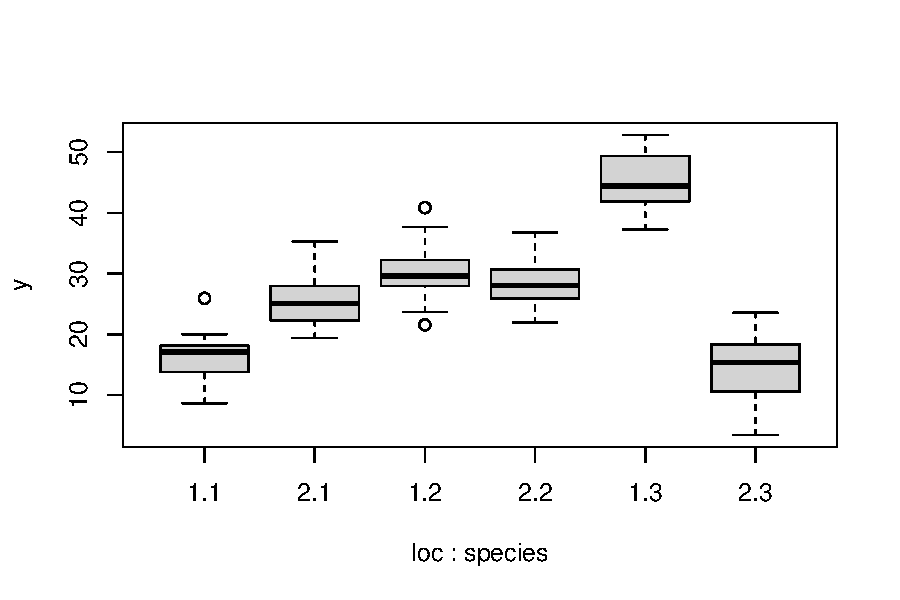
\includegraphics[keepaspectratio]{chapters/04-linear-models_files/figure-pdf/unnamed-chunk-12-1.pdf}}

The boxplot shows us what the interaction does. The effect of one factor
depends on the effect of another factor. Here, the effect of location is
different for each species:

\begin{itemize}
\tightlist
\item
  Location 2 has greater values than location 1 for species 1, smaller
  values than location 1 for species 3, and the same values as location
  1 for species 2.
\item
  In location 1, species 1 has the smallest values and species 3 has the
  greatest values. In location 2, species 3 has the smallest values and
  species 2 has the greatest values.
\end{itemize}

Another way to visualize this is with an \textbf{interaction plot}. This
shows the group means across every combination of factor levels. When
lines are parallel (or do not cross), then there is probably no
interaction. However, if lines do cross, then there is likely an
interaction and you need to test for it.

\begin{Shaded}
\begin{Highlighting}[]
\FunctionTok{par}\NormalTok{(}\AttributeTok{mfrow=}\FunctionTok{c}\NormalTok{(}\DecValTok{1}\NormalTok{,}\DecValTok{2}\NormalTok{), }\AttributeTok{bty=}\StringTok{"n"}\NormalTok{)}
\FunctionTok{interaction.plot}\NormalTok{(dx}\SpecialCharTok{$}\NormalTok{loc, dx}\SpecialCharTok{$}\NormalTok{species, dx}\SpecialCharTok{$}\NormalTok{y)}
\FunctionTok{interaction.plot}\NormalTok{(dx}\SpecialCharTok{$}\NormalTok{species, dx}\SpecialCharTok{$}\NormalTok{loc, dx}\SpecialCharTok{$}\NormalTok{y)}
\end{Highlighting}
\end{Shaded}

\pandocbounded{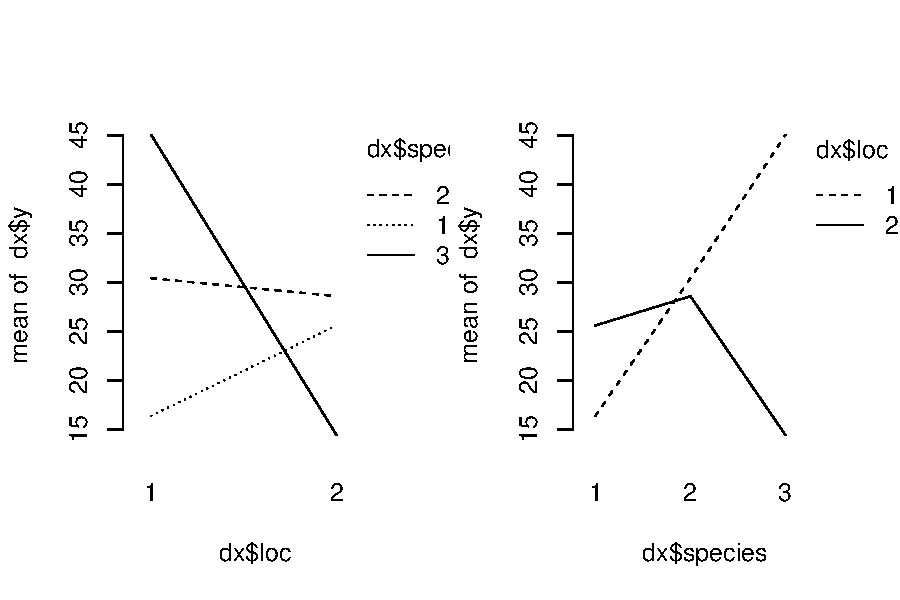
\includegraphics[keepaspectratio]{chapters/04-linear-models_files/figure-pdf/unnamed-chunk-13-1.pdf}}

We can fit a Bayesian ANOVA with interaction by using the means
parameterization of the model. This model can also be used to fit ANOVA
without interaction as well. Just as with some of the \emph{t}-tests
above, different readings of the model outputs can lead to different
versions of the test.

\begin{Shaded}
\begin{Highlighting}[]
\CommentTok{\#| label: fit{-}twowayanovainter{-}jags}
\CommentTok{\#| cache: true}

\FunctionTok{set.seed}\NormalTok{(}\DecValTok{123}\NormalTok{)}
\NormalTok{n }\OtherTok{\textless{}{-}} \DecValTok{20}
\NormalTok{dx }\OtherTok{\textless{}{-}} \FunctionTok{expand.grid}\NormalTok{(}\AttributeTok{species=}\DecValTok{1}\SpecialCharTok{:}\DecValTok{3}\NormalTok{,}
    \AttributeTok{loc=}\DecValTok{1}\SpecialCharTok{:}\DecValTok{2}\NormalTok{, }\AttributeTok{ind=}\DecValTok{1}\SpecialCharTok{:}\NormalTok{n)}
\NormalTok{dx}\SpecialCharTok{$}\NormalTok{y }\OtherTok{\textless{}{-}} \ConstantTok{NA}

\NormalTok{n }\OtherTok{\textless{}{-}} \FunctionTok{nrow}\NormalTok{(dx)}
\NormalTok{nspp }\OtherTok{\textless{}{-}} \DecValTok{3}
\NormalTok{nloc }\OtherTok{\textless{}{-}} \DecValTok{2}

\CommentTok{\# "true" means with interaction between spp and loc}
\NormalTok{mu }\OtherTok{\textless{}{-}} \FunctionTok{matrix}\NormalTok{(}\FunctionTok{c}\NormalTok{(}\DecValTok{15}\NormalTok{, }\DecValTok{30}\NormalTok{, }\DecValTok{45}\NormalTok{, }\DecValTok{25}\NormalTok{, }\DecValTok{30}\NormalTok{, }\DecValTok{15}\NormalTok{),}
    \AttributeTok{nrow=}\NormalTok{nspp, }\AttributeTok{ncol=}\NormalTok{nloc,}
    \AttributeTok{dimnames=}\FunctionTok{list}\NormalTok{(}
        \FunctionTok{paste0}\NormalTok{(}\StringTok{"spp"}\NormalTok{, }\DecValTok{1}\SpecialCharTok{:}\NormalTok{nspp),}
        \FunctionTok{paste}\NormalTok{(}\StringTok{"loc"}\NormalTok{, }\DecValTok{1}\SpecialCharTok{:}\NormalTok{nloc)))}

\CommentTok{\# residual SD}
\NormalTok{sigma.res }\OtherTok{\textless{}{-}} \DecValTok{5}

\CommentTok{\# draw y values given interaction and SD}
\ControlFlowTok{for}\NormalTok{(i }\ControlFlowTok{in} \DecValTok{1}\SpecialCharTok{:}\NormalTok{n)\{}
\NormalTok{    dx}\SpecialCharTok{$}\NormalTok{y[i] }\OtherTok{\textless{}{-}} \FunctionTok{rnorm}\NormalTok{(}\DecValTok{1}\NormalTok{, mu[dx}\SpecialCharTok{$}\NormalTok{species[i], dx}\SpecialCharTok{$}\NormalTok{loc[i]], sigma.res)}
\NormalTok{\}}

\CommentTok{\# means parameterization of two{-}way ANOVA}
\CommentTok{\# with interaction (works for without also)}
\NormalTok{mod.name }\OtherTok{\textless{}{-}} \StringTok{"jags\_anova2way\_means.txt"}
\FunctionTok{sink}\NormalTok{(mod.name)}
\FunctionTok{cat}\NormalTok{(}\StringTok{"}
\StringTok{    model\{}
\StringTok{        \# priors}
\StringTok{        for(i in 1:nfac1)\{}
\StringTok{            for(j in 1:nfac2)\{}
\StringTok{                mu[i,j] \textasciitilde{} dnorm(0, 0.001)}
\StringTok{            \}\#j}
\StringTok{        \}\#i}

\StringTok{        \#\# residual SD and precision}
\StringTok{        sigma \textasciitilde{} dlnorm(1, 0.25)}
\StringTok{        tau \textless{}{-} 1 / (sigma\^{}2)}

\StringTok{        \# likelihood}
\StringTok{        for(i in 1:n)\{}
\StringTok{            y[i] \textasciitilde{} dnorm(mu[fac1[i], fac2[i]], tau)}
\StringTok{        \}\#i}

\StringTok{    \}\#model}

\StringTok{"}\NormalTok{, }\AttributeTok{fill=}\ConstantTok{TRUE}\NormalTok{)}
\FunctionTok{sink}\NormalTok{()}

\CommentTok{\# parameters to monitor}
\NormalTok{params }\OtherTok{\textless{}{-}} \FunctionTok{c}\NormalTok{(}\StringTok{"mu"}\NormalTok{, }\StringTok{"sigma"}\NormalTok{)}

\CommentTok{\# MCMC parameters}
\NormalTok{n.iter }\OtherTok{\textless{}{-}} \FloatTok{5e4}
\NormalTok{n.burnin }\OtherTok{\textless{}{-}} \FloatTok{1e4}
\NormalTok{n.thin }\OtherTok{\textless{}{-}} \DecValTok{100}
\NormalTok{nchains }\OtherTok{\textless{}{-}} \DecValTok{3}

\CommentTok{\# reformat data for JAGS}
\NormalTok{fac1 }\OtherTok{\textless{}{-}}\NormalTok{ dx}\SpecialCharTok{$}\NormalTok{species}
\NormalTok{nfac1 }\OtherTok{\textless{}{-}} \FunctionTok{max}\NormalTok{(fac1)}
\NormalTok{fac2 }\OtherTok{\textless{}{-}}\NormalTok{ dx}\SpecialCharTok{$}\NormalTok{loc}
\NormalTok{nfac2 }\OtherTok{\textless{}{-}} \FunctionTok{max}\NormalTok{(fac2)}

\CommentTok{\# package data for JAGS}
\NormalTok{in.data }\OtherTok{\textless{}{-}} \FunctionTok{list}\NormalTok{(}\AttributeTok{y=}\NormalTok{dx}\SpecialCharTok{$}\NormalTok{y,}
    \AttributeTok{n=}\NormalTok{n,}
    \AttributeTok{fac1=}\NormalTok{fac1, }\AttributeTok{fac2=}\NormalTok{fac2,}
    \AttributeTok{nfac1=}\NormalTok{nfac1, }\AttributeTok{nfac2=}\NormalTok{nfac2)}

\CommentTok{\# function to define initial values for MCMC chains}
\NormalTok{init.fun }\OtherTok{\textless{}{-}} \ControlFlowTok{function}\NormalTok{(nc)\{}
\NormalTok{    res }\OtherTok{\textless{}{-}} \FunctionTok{vector}\NormalTok{(}\StringTok{"list"}\NormalTok{, }\AttributeTok{length=}\NormalTok{nc)}
    \ControlFlowTok{for}\NormalTok{(i }\ControlFlowTok{in} \DecValTok{1}\SpecialCharTok{:}\NormalTok{nc)\{}
\NormalTok{        res[[i]] }\OtherTok{\textless{}{-}} \FunctionTok{list}\NormalTok{(}\AttributeTok{mu=}\FunctionTok{matrix}\NormalTok{(}\FunctionTok{rnorm}\NormalTok{(nfac1}\SpecialCharTok{*}\NormalTok{nfac2, }\DecValTok{0}\NormalTok{, }\DecValTok{100}\NormalTok{),}
                             \AttributeTok{nrow=}\NormalTok{nfac1, }\AttributeTok{ncol=}\NormalTok{nfac2),}
                         \AttributeTok{sigma=}\FunctionTok{rlnorm}\NormalTok{(}\DecValTok{1}\NormalTok{, }\DecValTok{1}\NormalTok{, }\DecValTok{2}\NormalTok{))}
\NormalTok{    \}}
    \FunctionTok{return}\NormalTok{(res)}
\NormalTok{\}}
\NormalTok{inits }\OtherTok{\textless{}{-}} \FunctionTok{init.fun}\NormalTok{(nchains)}

\CommentTok{\# fit model}
\NormalTok{mod07 }\OtherTok{\textless{}{-}} \FunctionTok{jags}\NormalTok{(}\AttributeTok{data=}\NormalTok{in.data, }\AttributeTok{inits=}\NormalTok{inits,}
              \AttributeTok{parameters.to.save=}\NormalTok{params,}
              \AttributeTok{model.file=}\NormalTok{mod.name,}
              \AttributeTok{n.chains=}\NormalTok{nchains, }\AttributeTok{n.iter=}\NormalTok{n.iter,}
              \AttributeTok{n.burnin=}\NormalTok{n.burnin, }\AttributeTok{n.thin=}\NormalTok{n.thin)}\CommentTok{\#jags}
\end{Highlighting}
\end{Shaded}

\begin{verbatim}
Compiling model graph
   Resolving undeclared variables
   Allocating nodes
Graph information:
   Observed stochastic nodes: 120
   Unobserved stochastic nodes: 7
   Total graph size: 377

Initializing model
\end{verbatim}

\begin{Shaded}
\begin{Highlighting}[]
\NormalTok{mod07}
\end{Highlighting}
\end{Shaded}

\begin{verbatim}
Inference for Bugs model at "jags_anova2way_means.txt", fit using jags,
 3 chains, each with 50000 iterations (first 10000 discarded), n.thin = 100
 n.sims = 1200 iterations saved. Running time = 9.87 secs
         mu.vect sd.vect    2.5%     25%     50%     75%   97.5%  Rhat n.eff
mu[1,1]   16.416   1.005  14.441  15.734  16.450  17.110  18.233 1.004   550
mu[2,1]   30.378   0.994  28.510  29.673  30.373  31.028  32.372 1.004   680
mu[3,1]   45.018   1.020  43.084  44.307  45.013  45.691  47.008 1.002   920
mu[1,2]   25.626   0.977  23.778  24.948  25.610  26.285  27.510 1.001  1200
mu[2,2]   28.568   1.034  26.602  27.855  28.540  29.252  30.620 1.001  1200
mu[3,2]   14.395   1.026  12.443  13.681  14.385  15.084  16.431 1.001  1200
sigma      4.507   0.311   3.949   4.291   4.478   4.698   5.172 1.002   830
deviance 701.406   3.929 695.840 698.631 700.632 703.412 710.592 1.000  1200

For each parameter, n.eff is a crude measure of effective sample size,
and Rhat is the potential scale reduction factor (at convergence, Rhat=1).

DIC info (using the rule: pV = var(deviance)/2)
pV = 7.7 and DIC = 709.1
DIC is an estimate of expected predictive error (lower deviance is better).
\end{verbatim}

We can inspect the posteriors to see how the means differed among the 6
combinations of factor levels: species 1, location 1 (mu{[}1,1{]});
species 1, location 2 (mu{[}1,2{]}); and so on. Doing so would lead us
to discover the same interaction we suspected based on the interaction
plot above. A better way might be to visualize the group means using the
posteriors. Below is one way to do it:

\begin{Shaded}
\begin{Highlighting}[]
\CommentTok{\# get means and 95\% CRI for plot}
\NormalTok{res }\OtherTok{\textless{}{-}}\NormalTok{ mod07}\SpecialCharTok{$}\NormalTok{BUGSoutput}\SpecialCharTok{$}\NormalTok{summary}
\NormalTok{res1 }\OtherTok{\textless{}{-}}\NormalTok{ res[}\DecValTok{2}\SpecialCharTok{:}\DecValTok{4}\NormalTok{, }\FunctionTok{c}\NormalTok{(}\DecValTok{1}\NormalTok{, }\DecValTok{3}\NormalTok{, }\DecValTok{7}\NormalTok{)]}
\NormalTok{res2 }\OtherTok{\textless{}{-}}\NormalTok{ res[}\DecValTok{5}\SpecialCharTok{:}\DecValTok{7}\NormalTok{, }\FunctionTok{c}\NormalTok{(}\DecValTok{1}\NormalTok{, }\DecValTok{3}\NormalTok{, }\DecValTok{7}\NormalTok{)]}

\FunctionTok{par}\NormalTok{(}\AttributeTok{mfrow=}\FunctionTok{c}\NormalTok{(}\DecValTok{1}\NormalTok{,}\DecValTok{1}\NormalTok{), }\AttributeTok{mar=}\FunctionTok{c}\NormalTok{(}\FloatTok{5.1}\NormalTok{, }\FloatTok{8.1}\NormalTok{, }\FloatTok{1.1}\NormalTok{, }\FloatTok{1.1}\NormalTok{))}
\FunctionTok{plot}\NormalTok{(}\DecValTok{1}\SpecialCharTok{:}\DecValTok{2}\NormalTok{, }\AttributeTok{type=}\StringTok{"n"}\NormalTok{, }\AttributeTok{xlim=}\FunctionTok{c}\NormalTok{(}\DecValTok{10}\NormalTok{, }\DecValTok{50}\NormalTok{),}
    \AttributeTok{ylim=}\FunctionTok{c}\NormalTok{(}\DecValTok{0}\NormalTok{, }\FloatTok{3.5}\NormalTok{), }\AttributeTok{xlab=}\StringTok{"Posterior"}\NormalTok{,}
    \AttributeTok{yaxt=}\StringTok{"n"}\NormalTok{, }\AttributeTok{ylab=}\StringTok{""}\NormalTok{)}
\FunctionTok{segments}\NormalTok{(res1[,}\DecValTok{2}\NormalTok{], }\DecValTok{1}\SpecialCharTok{:}\DecValTok{3}\NormalTok{, res1[,}\DecValTok{3}\NormalTok{], }\DecValTok{1}\SpecialCharTok{:}\DecValTok{3}\NormalTok{, }\AttributeTok{lwd=}\DecValTok{3}\NormalTok{)}
\FunctionTok{segments}\NormalTok{(res2[,}\DecValTok{2}\NormalTok{], }\DecValTok{1}\SpecialCharTok{:}\DecValTok{3}\FloatTok{+0.2}\NormalTok{, res2[,}\DecValTok{3}\NormalTok{], }\DecValTok{1}\SpecialCharTok{:}\DecValTok{3}\FloatTok{+0.2}\NormalTok{, }\AttributeTok{lwd=}\DecValTok{3}\NormalTok{, }\AttributeTok{col=}\StringTok{"red"}\NormalTok{)}
\FunctionTok{points}\NormalTok{(res1[,}\DecValTok{1}\NormalTok{], }\DecValTok{1}\SpecialCharTok{:}\DecValTok{3}\NormalTok{, }\AttributeTok{pch=}\DecValTok{16}\NormalTok{, }\AttributeTok{cex=}\FloatTok{1.2}\NormalTok{)}
\FunctionTok{points}\NormalTok{(res2[,}\DecValTok{1}\NormalTok{], }\DecValTok{1}\SpecialCharTok{:}\DecValTok{3}\FloatTok{+0.2}\NormalTok{, }\AttributeTok{pch=}\DecValTok{16}\NormalTok{, }\AttributeTok{cex=}\FloatTok{1.2}\NormalTok{, }\AttributeTok{col=}\StringTok{"red"}\NormalTok{)}
\FunctionTok{legend}\NormalTok{(}\StringTok{"bottomright"}\NormalTok{, }\AttributeTok{legend=}\FunctionTok{paste}\NormalTok{(}\StringTok{"Location"}\NormalTok{, }\DecValTok{1}\SpecialCharTok{:}\DecValTok{2}\NormalTok{),}
    \AttributeTok{pch=}\DecValTok{16}\NormalTok{, }\AttributeTok{col=}\FunctionTok{c}\NormalTok{(}\StringTok{"black"}\NormalTok{, }\StringTok{"red"}\NormalTok{), }\AttributeTok{cex=}\FloatTok{1.2}\NormalTok{, }\AttributeTok{bty=}\StringTok{"n"}\NormalTok{)}
\FunctionTok{axis}\NormalTok{(}\AttributeTok{side=}\DecValTok{2}\NormalTok{, }\AttributeTok{at=}\DecValTok{1}\SpecialCharTok{:}\DecValTok{3}\FloatTok{+0.1}\NormalTok{, }\AttributeTok{labels=}\FunctionTok{paste}\NormalTok{(}\StringTok{"Species"}\NormalTok{, }\DecValTok{1}\SpecialCharTok{:}\DecValTok{3}\NormalTok{), }\AttributeTok{las=}\DecValTok{1}\NormalTok{)}
\FunctionTok{segments}\NormalTok{(}\DecValTok{10}\NormalTok{, }\DecValTok{1}\SpecialCharTok{:}\DecValTok{3}\FloatTok{+0.1}\NormalTok{, }\DecValTok{50}\NormalTok{, }\DecValTok{1}\SpecialCharTok{:}\DecValTok{3}\FloatTok{+0.1}\NormalTok{, }\AttributeTok{lty=}\DecValTok{2}\NormalTok{)}
\end{Highlighting}
\end{Shaded}

\pandocbounded{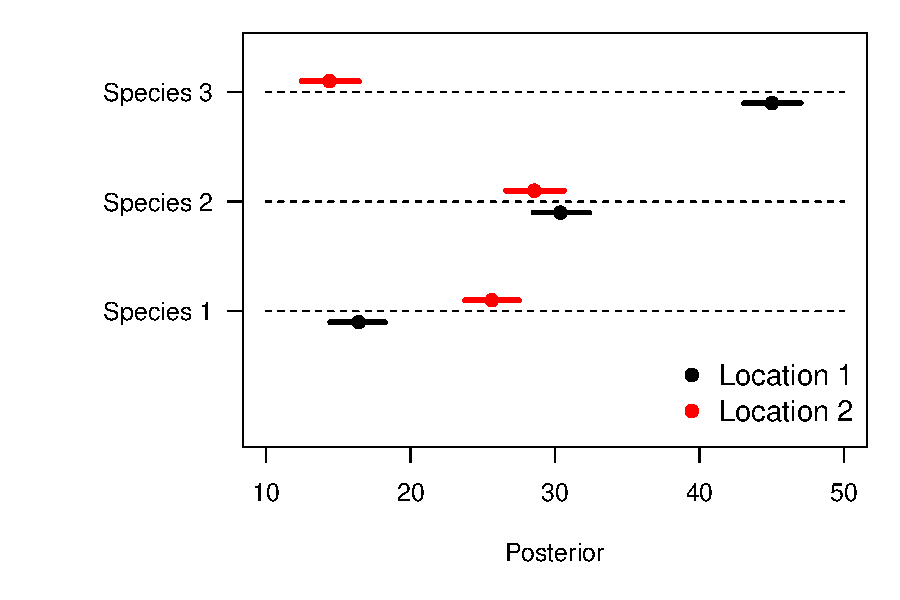
\includegraphics[keepaspectratio]{chapters/04-linear-models_files/figure-pdf/unnamed-chunk-15-1.pdf}}

\section{Continuous patterns}\label{continuous-patterns}

\subsection{Linear regression}\label{linear-regression}

One of the most well-known of all statistical analyses, the linear
regression model describes a pattern where some response variable \(y\)
varies as a linear function of a predictor variable \(x\). The equation
is:

\[y=\beta_0+\beta_1x+\varepsilon\]

where: - \(y\) is the response or dependent variable - \(x\) is the
explanatory, predictor, or independent variable - \(\beta_0\) is the
\emph{y}-intercept (i.e., the value of \(y\) when \(x = 0\)) (``beta
zero'' or ``beta naught'') - \(\beta_1\) is the slope or regression
coefficient (i.e., the change in \(y\) per unit change in \(x\)) (``beta
one''). If \(x\) increases by 1, then y increases by \(\beta_1\). -
\(\varepsilon\) is a random error term that describes residual variation
not explained by the model (``epsilon'').

When we specify the model in JAGS, we do so using an observation-wise,
state-space notation.

\[y_i~Normal\left(\eta_i,\ \sigma_{res}\right)\]

\[\eta_i=\beta_0+\beta_1x_i\]

This format makes it clear that each y value has its own expected value
\(\eta_i\) (``eta sub i''), dependent on that observation's \(x\) value
\(x_i\). This relates to a key assumption of the linear model, that
residuals are independently and identically distributed (i.i.d.). It
also echoes the way we program the model likelihood in JAGS, a for loop.

The ``state-space'' part of the formulation above refers to the fact
that the model equation explicitly spearates the true, unobserved,
``state'' of the system from the observed values which occur in a
``space'' defined by the state and the uncertainty about the observation
process.

\subsubsection{Linear regression in
JAGS}\label{linear-regression-in-jags}

The procedure for linear regression in JAGS is very similar to the
procedure for the effects parameterization of the two-way ANOVA that we
saw in section X. As we'll soon see, this is also very similar to how
we'll fit a wide variety of models for the rest of the course---linear
or otherwise.

\begin{Shaded}
\begin{Highlighting}[]
\FunctionTok{library}\NormalTok{(rjags)}
\FunctionTok{library}\NormalTok{(R2jags)}
\CommentTok{\# simulate some data}
\FunctionTok{set.seed}\NormalTok{(}\DecValTok{42}\NormalTok{)}
\NormalTok{n }\OtherTok{\textless{}{-}} \DecValTok{50}
\NormalTok{dx }\OtherTok{\textless{}{-}} \FunctionTok{data.frame}\NormalTok{(}\AttributeTok{x=}\FunctionTok{runif}\NormalTok{(n, }\DecValTok{0}\NormalTok{, }\DecValTok{20}\NormalTok{))}

\NormalTok{beta0 }\OtherTok{\textless{}{-}} \DecValTok{4}
\NormalTok{beta1 }\OtherTok{\textless{}{-}} \FloatTok{1.8}
\NormalTok{sigma.res }\OtherTok{\textless{}{-}} \DecValTok{4}
\NormalTok{dx}\SpecialCharTok{$}\NormalTok{y }\OtherTok{\textless{}{-}}\NormalTok{ beta0 }\SpecialCharTok{+}\NormalTok{ beta1}\SpecialCharTok{*}\NormalTok{dx}\SpecialCharTok{$}\NormalTok{x }\SpecialCharTok{+} \FunctionTok{rnorm}\NormalTok{(n, }\DecValTok{0}\NormalTok{, sigma.res)}

\CommentTok{\# linear regression with 1 predictor}
\NormalTok{mod.name }\OtherTok{\textless{}{-}} \StringTok{"jags\_linreg\_1x.txt"}
\FunctionTok{sink}\NormalTok{(mod.name)}
\FunctionTok{cat}\NormalTok{(}\StringTok{"}
\StringTok{    model\{}
\StringTok{        \# priors}
\StringTok{        \#\# intercept}
\StringTok{        beta0 \textasciitilde{} dnorm(0, 0.001)}

\StringTok{        \#\# slope}
\StringTok{        beta1 \textasciitilde{} dnorm(0, 0.001)}

\StringTok{        \#\# residual SD and precision}
\StringTok{        sigma \textasciitilde{} dlnorm(1, 0.25)}
\StringTok{        tau \textless{}{-} 1 / (sigma\^{}2)}

\StringTok{        \# likelihood}
\StringTok{        \# (for loop)}
\StringTok{        for(i in 1:n)\{}
\StringTok{            y[i] \textasciitilde{} dnorm(eta[i], tau)}
\StringTok{            eta[i] \textless{}{-} beta0 + beta1 * x[i]}
\StringTok{        \}\#i}

\StringTok{    \}\#model}

\StringTok{"}\NormalTok{, }\AttributeTok{fill=}\ConstantTok{TRUE}\NormalTok{)}
\FunctionTok{sink}\NormalTok{()}

\CommentTok{\# parameters to monitor}
\NormalTok{params }\OtherTok{\textless{}{-}} \FunctionTok{c}\NormalTok{(}\StringTok{"beta0"}\NormalTok{, }\StringTok{"beta1"}\NormalTok{, }\StringTok{"sigma"}\NormalTok{)}

\CommentTok{\# MCMC parameters}
\NormalTok{n.iter }\OtherTok{\textless{}{-}} \FloatTok{5e4}
\NormalTok{n.burnin }\OtherTok{\textless{}{-}} \FloatTok{1e4}
\NormalTok{n.thin }\OtherTok{\textless{}{-}} \DecValTok{100}
\NormalTok{nchains }\OtherTok{\textless{}{-}} \DecValTok{3}

\CommentTok{\# package data for JAGS}
\NormalTok{in.data }\OtherTok{\textless{}{-}} \FunctionTok{list}\NormalTok{(}\AttributeTok{y=}\NormalTok{dx}\SpecialCharTok{$}\NormalTok{y,}
    \AttributeTok{n=}\NormalTok{n, }\AttributeTok{x=}\NormalTok{dx}\SpecialCharTok{$}\NormalTok{x)}

\CommentTok{\# function to define initial values for MCMC chains}
\NormalTok{init.fun }\OtherTok{\textless{}{-}} \ControlFlowTok{function}\NormalTok{(nc)\{}
\NormalTok{    res }\OtherTok{\textless{}{-}} \FunctionTok{vector}\NormalTok{(}\StringTok{"list"}\NormalTok{, }\AttributeTok{length=}\NormalTok{nc)}
    \ControlFlowTok{for}\NormalTok{(i }\ControlFlowTok{in} \DecValTok{1}\SpecialCharTok{:}\NormalTok{nc)\{}
\NormalTok{        res[[i]] }\OtherTok{\textless{}{-}} \FunctionTok{list}\NormalTok{(}\AttributeTok{beta0=}\FunctionTok{rnorm}\NormalTok{(}\DecValTok{1}\NormalTok{, }\DecValTok{0}\NormalTok{, }\DecValTok{100}\NormalTok{),}
                         \AttributeTok{beta1=}\FunctionTok{rnorm}\NormalTok{(}\DecValTok{1}\NormalTok{, }\DecValTok{0}\NormalTok{, }\DecValTok{100}\NormalTok{),}
                         \AttributeTok{sigma=}\FunctionTok{rlnorm}\NormalTok{(}\DecValTok{1}\NormalTok{, }\DecValTok{1}\NormalTok{, }\DecValTok{2}\NormalTok{))}
\NormalTok{    \}}
    \FunctionTok{return}\NormalTok{(res)}
\NormalTok{\}}
\NormalTok{inits }\OtherTok{\textless{}{-}} \FunctionTok{init.fun}\NormalTok{(nchains)}

\CommentTok{\# fit model}
\NormalTok{mod08 }\OtherTok{\textless{}{-}} \FunctionTok{jags}\NormalTok{(}\AttributeTok{data=}\NormalTok{in.data, }\AttributeTok{inits=}\NormalTok{inits,}
              \AttributeTok{parameters.to.save=}\NormalTok{params,}
              \AttributeTok{model.file=}\NormalTok{mod.name,}
              \AttributeTok{n.chains=}\NormalTok{nchains, }\AttributeTok{n.iter=}\NormalTok{n.iter,}
              \AttributeTok{n.burnin=}\NormalTok{n.burnin, }\AttributeTok{n.thin=}\NormalTok{n.thin)}\CommentTok{\#jags}
\end{Highlighting}
\end{Shaded}

\begin{verbatim}
Compiling model graph
   Resolving undeclared variables
   Allocating nodes
Graph information:
   Observed stochastic nodes: 50
   Unobserved stochastic nodes: 3
   Total graph size: 211

Initializing model
\end{verbatim}

\begin{Shaded}
\begin{Highlighting}[]
\NormalTok{mod08}
\end{Highlighting}
\end{Shaded}

\begin{verbatim}
Inference for Bugs model at "jags_linreg_1x.txt", fit using jags,
 3 chains, each with 50000 iterations (first 10000 discarded), n.thin = 100
 n.sims = 1200 iterations saved. Running time = 5.5 secs
         mu.vect sd.vect    2.5%     25%     50%     75%   97.5%  Rhat n.eff
beta0      3.854   1.313   1.312   3.002   3.863   4.724   6.458 1.001  1200
beta1      1.791   0.096   1.602   1.725   1.790   1.855   1.984 1.001  1200
sigma      3.995   0.439   3.227   3.681   3.970   4.260   4.965 1.000  1200
deviance 279.763   2.600 276.746 277.844 279.052 281.041 286.526 1.003  1200

For each parameter, n.eff is a crude measure of effective sample size,
and Rhat is the potential scale reduction factor (at convergence, Rhat=1).

DIC info (using the rule: pV = var(deviance)/2)
pV = 3.4 and DIC = 283.1
DIC is an estimate of expected predictive error (lower deviance is better).
\end{verbatim}

The outputs show that the posterior means for beta0 and beta1 are
reasonably close to the truth (3.843 vs.~4, and 1.791 vs.~1.8) and the
estimates from the frequentist model fit in R. The true values are well
within the 95\% CRI.

The next step is to produce a plot of the model's predicted values and
95\% CRI. As we'll see, this is a little more involved than the process
in R. But, we'll practice the process so much that it will seem easy by
the end of the course!

\subsubsection{Plotting model predictions in
R}\label{plotting-model-predictions-in-r}

The basic procedure for plotting a linear model and its predictions in R
is as follows: 1. Fit the model and save it to a model object. 1.
Generate predicted values and SE of predicted values over a range of x
values that cover the range of observed x. 1. Use the predicted values
and SE to calculate 95\% confidence intervals (CI) of the predictions.
1. Plot the predictions and 95\% CI.

Here is what that looks like:

\begin{Shaded}
\begin{Highlighting}[]
\CommentTok{\# fit the model}
\NormalTok{mod08fr }\OtherTok{\textless{}{-}} \FunctionTok{lm}\NormalTok{(y}\SpecialCharTok{\textasciitilde{}}\NormalTok{x, }\AttributeTok{data=}\NormalTok{dx)}

\CommentTok{\# new data for prediction}
\NormalTok{px }\OtherTok{\textless{}{-}} \FunctionTok{seq}\NormalTok{(}\FunctionTok{min}\NormalTok{(dx}\SpecialCharTok{$}\NormalTok{x), }\FunctionTok{max}\NormalTok{(dx}\SpecialCharTok{$}\NormalTok{x), }\AttributeTok{length=}\DecValTok{100}\NormalTok{)}

\CommentTok{\# prediction with expected mean and SE of Y}
\NormalTok{pred }\OtherTok{\textless{}{-}} \FunctionTok{predict}\NormalTok{(mod08fr, }\AttributeTok{newdata=}\FunctionTok{data.frame}\NormalTok{(}\AttributeTok{x=}\NormalTok{px),}
                \AttributeTok{se.fit=}\ConstantTok{TRUE}\NormalTok{, }\AttributeTok{interval=}\StringTok{"confidence"}\NormalTok{)}

\CommentTok{\# predicted mean and 95\% CI}
\NormalTok{y.lo }\OtherTok{\textless{}{-}}\NormalTok{ pred}\SpecialCharTok{$}\NormalTok{fit[,}\DecValTok{2}\NormalTok{]}
\NormalTok{y.mn }\OtherTok{\textless{}{-}}\NormalTok{ pred}\SpecialCharTok{$}\NormalTok{fit[,}\DecValTok{1}\NormalTok{]}
\NormalTok{y.up }\OtherTok{\textless{}{-}}\NormalTok{ pred}\SpecialCharTok{$}\NormalTok{fit[,}\DecValTok{3}\NormalTok{]}

\CommentTok{\# fancy plot options with par()}
\FunctionTok{par}\NormalTok{(}\AttributeTok{mfrow=}\FunctionTok{c}\NormalTok{(}\DecValTok{1}\NormalTok{,}\DecValTok{1}\NormalTok{), }\AttributeTok{mar=}\FunctionTok{c}\NormalTok{(}\FloatTok{5.1}\NormalTok{, }\FloatTok{5.1}\NormalTok{, }\FloatTok{1.1}\NormalTok{, }\FloatTok{1.1}\NormalTok{),}
    \AttributeTok{bty=}\StringTok{"n"}\NormalTok{, }\AttributeTok{lend=}\DecValTok{1}\NormalTok{,}
    \AttributeTok{las=}\DecValTok{1}\NormalTok{, }\AttributeTok{cex.axis=}\FloatTok{1.2}\NormalTok{, }\AttributeTok{cex.lab=}\FloatTok{1.2}\NormalTok{)}
\CommentTok{\# make the plot and set basic options}
\FunctionTok{plot}\NormalTok{(dx}\SpecialCharTok{$}\NormalTok{x, dx}\SpecialCharTok{$}\NormalTok{y, }\AttributeTok{type=}\StringTok{"n"}\NormalTok{,}
    \AttributeTok{ylim=}\FunctionTok{c}\NormalTok{(}\DecValTok{0}\NormalTok{, }\DecValTok{50}\NormalTok{), }\AttributeTok{xlim=}\FunctionTok{c}\NormalTok{(}\DecValTok{0}\NormalTok{, }\DecValTok{20}\NormalTok{),}
    \AttributeTok{xlab=}\StringTok{"x variable"}\NormalTok{, }\AttributeTok{ylab=}\StringTok{"y variable"}\NormalTok{)}
\CommentTok{\# add lines for lower, upper conf. limits}
\CommentTok{\# and predicted mean}
\FunctionTok{points}\NormalTok{(px, y.lo, }\AttributeTok{type=}\StringTok{"l"}\NormalTok{, }\AttributeTok{lwd=}\DecValTok{2}\NormalTok{, }\AttributeTok{lty=}\DecValTok{2}\NormalTok{) }
\FunctionTok{points}\NormalTok{(px, y.up, }\AttributeTok{type=}\StringTok{"l"}\NormalTok{, }\AttributeTok{lwd=}\DecValTok{2}\NormalTok{, }\AttributeTok{lty=}\DecValTok{2}\NormalTok{) }
\FunctionTok{points}\NormalTok{(px, y.mn, }\AttributeTok{type=}\StringTok{"l"}\NormalTok{, }\AttributeTok{lwd=}\DecValTok{2}\NormalTok{)}
\CommentTok{\# put original data on top, so not covered by }
\CommentTok{\# lines and etc.}
\FunctionTok{points}\NormalTok{(dx}\SpecialCharTok{$}\NormalTok{x, dx}\SpecialCharTok{$}\NormalTok{y, }\AttributeTok{pch=}\DecValTok{16}\NormalTok{, }\AttributeTok{cex=}\FloatTok{1.2}\NormalTok{)}
\end{Highlighting}
\end{Shaded}

\pandocbounded{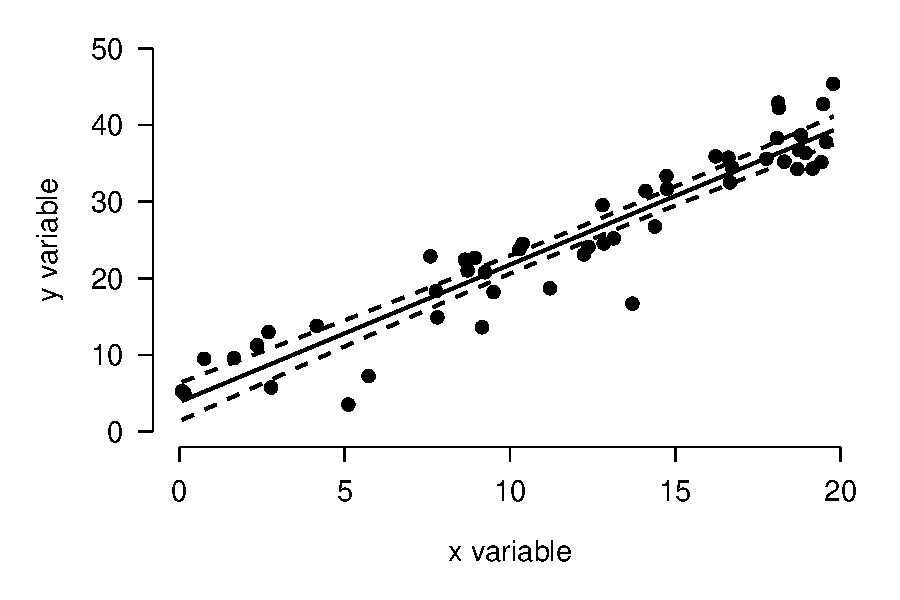
\includegraphics[keepaspectratio]{chapters/04-linear-models_files/figure-pdf/unnamed-chunk-16-1.pdf}}

We will have to perform the same basic steps to produce a similar plot
from JAGS, but the implementation is a bit different because there isn't
a good \texttt{predict()} method in R for these kinds of models .

We are going to use the posterior draws for each parameter. To avoid
issues with autocorrelation in the chains, we will pull these from
\texttt{sims.matrix} instead of \texttt{sims.array}. These values have
been permuted from the raw MCMC outputs so that predicted values do not
suffer from any potential issues of autocorrelation in the chains or
cross-correlations between the posteriors of different parameters.

\begin{Shaded}
\begin{Highlighting}[]
\CommentTok{\# matrix of coefficients}
\NormalTok{prx }\OtherTok{\textless{}{-}}\NormalTok{ mod08}\SpecialCharTok{$}\NormalTok{BUGSoutput}\SpecialCharTok{$}\NormalTok{sims.matrix}
\DocumentationTok{\#\# don\textquotesingle{}t need deviance or sigma}
\NormalTok{prx }\OtherTok{\textless{}{-}}\NormalTok{ prx[,}\FunctionTok{c}\NormalTok{(}\StringTok{"beta0"}\NormalTok{, }\StringTok{"beta1"}\NormalTok{)]}
\NormalTok{post.n }\OtherTok{\textless{}{-}} \FunctionTok{nrow}\NormalTok{(prx)}
\end{Highlighting}
\end{Shaded}

Next, we need a vector of x values at which to predict using the model.
As before, we'll set up a series of values at small intervals over the
full range of observed x.

\begin{Shaded}
\begin{Highlighting}[]
\CommentTok{\# x values at which to predict}
\NormalTok{pred.n }\OtherTok{\textless{}{-}} \DecValTok{100}
\NormalTok{px }\OtherTok{\textless{}{-}} \FunctionTok{seq}\NormalTok{(}\FunctionTok{min}\NormalTok{(dx}\SpecialCharTok{$}\NormalTok{x), }\FunctionTok{max}\NormalTok{(dx}\SpecialCharTok{$}\NormalTok{x), }\AttributeTok{length=}\NormalTok{pred.n)}
\end{Highlighting}
\end{Shaded}

If you are familiar with matrix multiplication, the matrix of
predictions can be obtained very quickly by constructing the design
matrix and multiplying it by the transpose of the coefficients matrix:

\begin{Shaded}
\begin{Highlighting}[]
\NormalTok{design.mat }\OtherTok{\textless{}{-}} \FunctionTok{matrix}\NormalTok{(}\FunctionTok{c}\NormalTok{(}\FunctionTok{rep}\NormalTok{(}\DecValTok{1}\NormalTok{, pred.n), px), }\AttributeTok{ncol=}\DecValTok{2}\NormalTok{)}
\NormalTok{pred.mat }\OtherTok{\textless{}{-}}\NormalTok{ design.mat }\SpecialCharTok{\%*\%} \FunctionTok{t}\NormalTok{(prx)}
\end{Highlighting}
\end{Shaded}

In my experience, the easier and more flexible approach is to calculate
the predicted values in a loop (the above only works with ordinary
linear models). Set up a matrix to hold the predicted values for each
posterior draw of the predictors, and for each value of the predictor
variable at which we want a prediction. This part is a bit tricky, so
consider the figure below. The plan here is to end up with the predictor
values along one margin (rows) and the replicates along the other
(columns) . Once the matrix is filled, we can use \texttt{apply()} to
get quantiles of the predicted values for each x.

\begin{figure}

\caption{\label{fig-linearpredict}Relationship between objects used to
calculate model predictions and their 95\% confidence interval (CI).}

\centering{

\pandocbounded{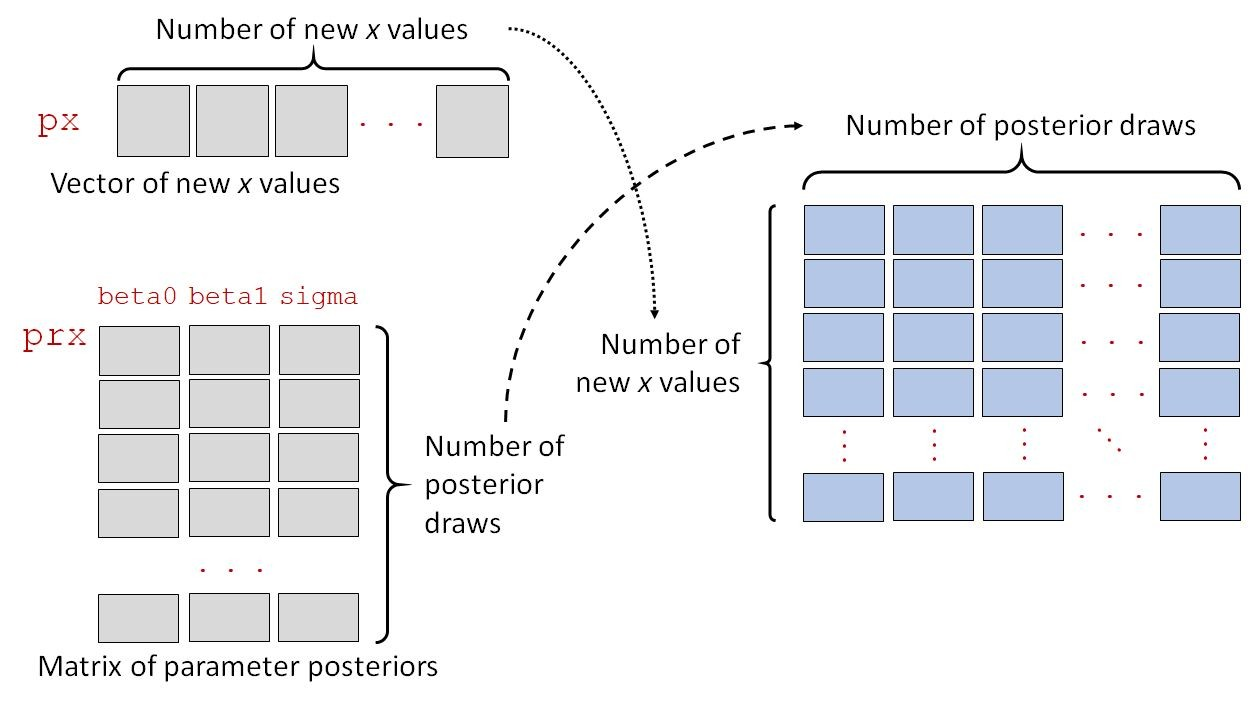
\includegraphics[keepaspectratio,alt={Figure showing the relationship between the objects used to calculate the predicted values from a linear regression from the matrix of posterior draws of each parameter in sims.array, a vector px of new x values, and a data frame prx that contains predictors and model parameters across model posteriors.}]{chapters/../images/06-02.jpg}}

}

\end{figure}%

\begin{Shaded}
\begin{Highlighting}[]
\CommentTok{\# set up matrix}
\NormalTok{pred.mat }\OtherTok{\textless{}{-}} \FunctionTok{matrix}\NormalTok{(}\ConstantTok{NA}\NormalTok{, }\AttributeTok{nrow=}\NormalTok{pred.n, }\AttributeTok{ncol=}\NormalTok{post.n)}

\CommentTok{\# fill in a loop}
\ControlFlowTok{for}\NormalTok{(i }\ControlFlowTok{in} \DecValTok{1}\SpecialCharTok{:}\NormalTok{post.n)\{}
\NormalTok{    pred.mat[,i] }\OtherTok{\textless{}{-}}\NormalTok{ prx[i,}\StringTok{"beta0"}\NormalTok{] }\SpecialCharTok{+}\NormalTok{ prx[i,}\StringTok{"beta1"}\NormalTok{] }\SpecialCharTok{*}\NormalTok{ px}
\NormalTok{\}}\CommentTok{\#i}
\end{Highlighting}
\end{Shaded}

No matter how the predicted values for every new x were calculated, we
can get the mean and 95\% CRI using the mean and quantile functions.
Sometimes I'll use the posterior median instead of the mean. For linear
models it doesn't matter, but for models with other response
distributions the median can be more representative of the central
tendency.

\begin{Shaded}
\begin{Highlighting}[]
\CommentTok{\# set up data frame with mean and CRI}
\NormalTok{plotdf }\OtherTok{\textless{}{-}} \FunctionTok{data.frame}\NormalTok{(}\AttributeTok{x=}\NormalTok{px,}
    \AttributeTok{mn=}\FunctionTok{apply}\NormalTok{(pred.mat, }\DecValTok{1}\NormalTok{, mean),}
    \AttributeTok{lo=}\FunctionTok{apply}\NormalTok{(pred.mat, }\DecValTok{1}\NormalTok{, quantile, }\FloatTok{0.025}\NormalTok{),}
    \AttributeTok{up=}\FunctionTok{apply}\NormalTok{(pred.mat, }\DecValTok{1}\NormalTok{, quantile, }\FloatTok{0.975}\NormalTok{))}
\end{Highlighting}
\end{Shaded}

We can use our new object \texttt{plotdf} to make a nice plot of the
model predictions. The code is almost identical to the code for the
frequentist model outputs shown above because we set up the objects
containing the plot values in the same way.

\begin{Shaded}
\begin{Highlighting}[]
\CommentTok{\# fancy plot options with par()}
\FunctionTok{par}\NormalTok{(}\AttributeTok{mfrow=}\FunctionTok{c}\NormalTok{(}\DecValTok{1}\NormalTok{,}\DecValTok{1}\NormalTok{), }\AttributeTok{mar=}\FunctionTok{c}\NormalTok{(}\FloatTok{5.1}\NormalTok{, }\FloatTok{5.1}\NormalTok{, }\FloatTok{1.1}\NormalTok{, }\FloatTok{1.1}\NormalTok{),}
    \AttributeTok{bty=}\StringTok{"n"}\NormalTok{, }\AttributeTok{lend=}\DecValTok{1}\NormalTok{,}
    \AttributeTok{las=}\DecValTok{1}\NormalTok{, }\AttributeTok{cex.axis=}\FloatTok{1.2}\NormalTok{, }\AttributeTok{cex.lab=}\FloatTok{1.2}\NormalTok{)}
\CommentTok{\# make the plot and set basic options}
\FunctionTok{plot}\NormalTok{(dx}\SpecialCharTok{$}\NormalTok{x, dx}\SpecialCharTok{$}\NormalTok{y, }\AttributeTok{type=}\StringTok{"n"}\NormalTok{,}
    \AttributeTok{ylim=}\FunctionTok{c}\NormalTok{(}\DecValTok{0}\NormalTok{, }\DecValTok{50}\NormalTok{), }\AttributeTok{xlim=}\FunctionTok{c}\NormalTok{(}\DecValTok{0}\NormalTok{, }\DecValTok{20}\NormalTok{),}
    \AttributeTok{xlab=}\StringTok{"x variable"}\NormalTok{, }\AttributeTok{ylab=}\StringTok{"y variable"}\NormalTok{)}
\CommentTok{\# add lines for lower, upper conf. limits}
\CommentTok{\# and predicted mean}
\FunctionTok{points}\NormalTok{(plotdf}\SpecialCharTok{$}\NormalTok{x, plotdf}\SpecialCharTok{$}\NormalTok{lo, }\AttributeTok{type=}\StringTok{"l"}\NormalTok{, }\AttributeTok{lwd=}\DecValTok{2}\NormalTok{, }\AttributeTok{lty=}\DecValTok{2}\NormalTok{) }
\FunctionTok{points}\NormalTok{(plotdf}\SpecialCharTok{$}\NormalTok{x, plotdf}\SpecialCharTok{$}\NormalTok{up, }\AttributeTok{type=}\StringTok{"l"}\NormalTok{, }\AttributeTok{lwd=}\DecValTok{2}\NormalTok{, }\AttributeTok{lty=}\DecValTok{2}\NormalTok{) }
\FunctionTok{points}\NormalTok{(plotdf}\SpecialCharTok{$}\NormalTok{x, plotdf}\SpecialCharTok{$}\NormalTok{mn, }\AttributeTok{type=}\StringTok{"l"}\NormalTok{, }\AttributeTok{lwd=}\DecValTok{2}\NormalTok{)}
\CommentTok{\# put original data on top, so not covered by }
\CommentTok{\# lines and etc.}
\FunctionTok{points}\NormalTok{(dx}\SpecialCharTok{$}\NormalTok{x, dx}\SpecialCharTok{$}\NormalTok{y, }\AttributeTok{pch=}\DecValTok{16}\NormalTok{, }\AttributeTok{cex=}\FloatTok{1.2}\NormalTok{)}
\end{Highlighting}
\end{Shaded}

\pandocbounded{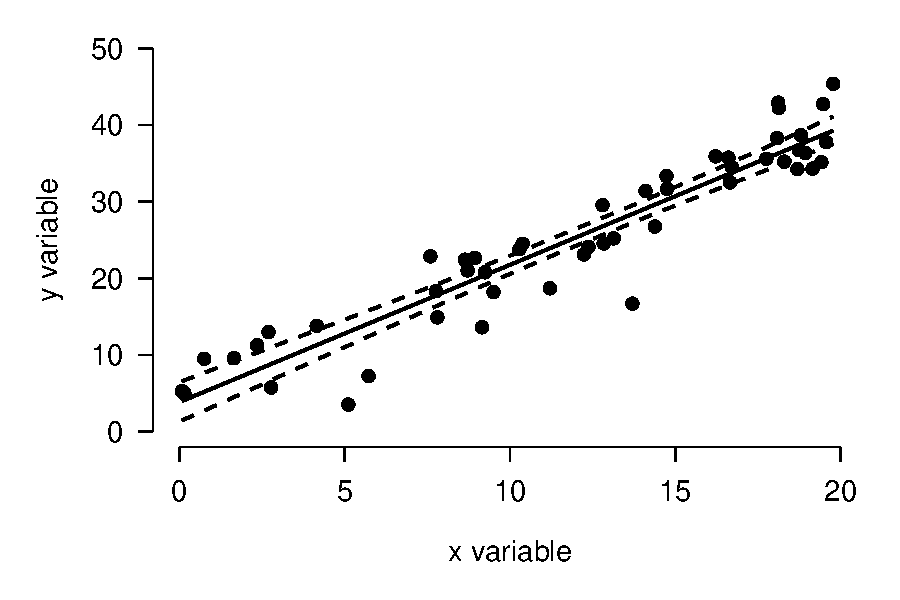
\includegraphics[keepaspectratio]{chapters/04-linear-models_files/figure-pdf/unnamed-chunk-22-1.pdf}}

If you add the frequentist predictions and CI with the following
commands, you'll see that they are nearly the same as the Bayesian
prediction and CRI.

\begin{Shaded}
\begin{Highlighting}[]
\CommentTok{\# fancy plot options with par()}
\FunctionTok{par}\NormalTok{(}\AttributeTok{mfrow=}\FunctionTok{c}\NormalTok{(}\DecValTok{1}\NormalTok{,}\DecValTok{1}\NormalTok{), }\AttributeTok{mar=}\FunctionTok{c}\NormalTok{(}\FloatTok{5.1}\NormalTok{, }\FloatTok{5.1}\NormalTok{, }\FloatTok{1.1}\NormalTok{, }\FloatTok{1.1}\NormalTok{),}
    \AttributeTok{bty=}\StringTok{"n"}\NormalTok{, }\AttributeTok{lend=}\DecValTok{1}\NormalTok{,}
    \AttributeTok{las=}\DecValTok{1}\NormalTok{, }\AttributeTok{cex.axis=}\FloatTok{1.2}\NormalTok{, }\AttributeTok{cex.lab=}\FloatTok{1.2}\NormalTok{)}
\CommentTok{\# make the plot and set basic options}
\FunctionTok{plot}\NormalTok{(dx}\SpecialCharTok{$}\NormalTok{x, dx}\SpecialCharTok{$}\NormalTok{y, }\AttributeTok{type=}\StringTok{"n"}\NormalTok{,}
    \AttributeTok{ylim=}\FunctionTok{c}\NormalTok{(}\DecValTok{0}\NormalTok{, }\DecValTok{50}\NormalTok{), }\AttributeTok{xlim=}\FunctionTok{c}\NormalTok{(}\DecValTok{0}\NormalTok{, }\DecValTok{20}\NormalTok{),}
    \AttributeTok{xlab=}\StringTok{"x variable"}\NormalTok{, }\AttributeTok{ylab=}\StringTok{"y variable"}\NormalTok{)}
\CommentTok{\# add lines for lower, upper conf. limits}
\CommentTok{\# and predicted mean}
\FunctionTok{points}\NormalTok{(plotdf}\SpecialCharTok{$}\NormalTok{x, plotdf}\SpecialCharTok{$}\NormalTok{lo, }\AttributeTok{type=}\StringTok{"l"}\NormalTok{, }\AttributeTok{lwd=}\DecValTok{2}\NormalTok{, }\AttributeTok{lty=}\DecValTok{2}\NormalTok{) }
\FunctionTok{points}\NormalTok{(plotdf}\SpecialCharTok{$}\NormalTok{x, plotdf}\SpecialCharTok{$}\NormalTok{up, }\AttributeTok{type=}\StringTok{"l"}\NormalTok{, }\AttributeTok{lwd=}\DecValTok{2}\NormalTok{, }\AttributeTok{lty=}\DecValTok{2}\NormalTok{) }
\FunctionTok{points}\NormalTok{(plotdf}\SpecialCharTok{$}\NormalTok{x, plotdf}\SpecialCharTok{$}\NormalTok{mn, }\AttributeTok{type=}\StringTok{"l"}\NormalTok{, }\AttributeTok{lwd=}\DecValTok{2}\NormalTok{)}
\CommentTok{\# put original data on top, so not covered by }
\CommentTok{\# lines and etc.}
\FunctionTok{points}\NormalTok{(dx}\SpecialCharTok{$}\NormalTok{x, dx}\SpecialCharTok{$}\NormalTok{y, }\AttributeTok{pch=}\DecValTok{16}\NormalTok{, }\AttributeTok{cex=}\FloatTok{1.2}\NormalTok{)}
\CommentTok{\# add frequentist interval for comparison}
\FunctionTok{points}\NormalTok{(px, y.lo, }\AttributeTok{type=}\StringTok{"l"}\NormalTok{, }\AttributeTok{lwd=}\DecValTok{2}\NormalTok{, }\AttributeTok{lty=}\DecValTok{2}\NormalTok{, }\AttributeTok{col=}\StringTok{"red"}\NormalTok{) }
\FunctionTok{points}\NormalTok{(px, y.up, }\AttributeTok{type=}\StringTok{"l"}\NormalTok{, }\AttributeTok{lwd=}\DecValTok{2}\NormalTok{, }\AttributeTok{lty=}\DecValTok{2}\NormalTok{, }\AttributeTok{col=}\StringTok{"red"}\NormalTok{) }
\FunctionTok{points}\NormalTok{(px, y.mn, }\AttributeTok{type=}\StringTok{"l"}\NormalTok{, }\AttributeTok{lwd=}\DecValTok{2}\NormalTok{, }\AttributeTok{col=}\StringTok{"red"}\NormalTok{)}
\FunctionTok{legend}\NormalTok{(}\StringTok{"topleft"}\NormalTok{, }\AttributeTok{legend=}\FunctionTok{c}\NormalTok{(}\StringTok{"Frequentist"}\NormalTok{, }\StringTok{"Bayesian"}\NormalTok{),}
    \AttributeTok{lwd=}\DecValTok{3}\NormalTok{, }\AttributeTok{col=}\FunctionTok{c}\NormalTok{(}\StringTok{"red"}\NormalTok{, }\StringTok{"black"}\NormalTok{))}
\end{Highlighting}
\end{Shaded}

\pandocbounded{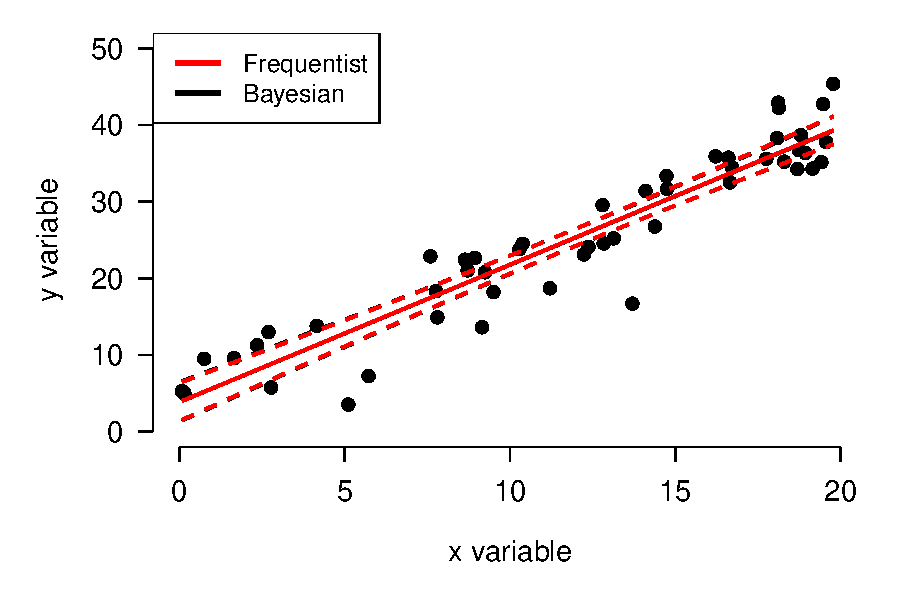
\includegraphics[keepaspectratio]{chapters/04-linear-models_files/figure-pdf/unnamed-chunk-23-1.pdf}}

\subsection{Multiple linear
regression}\label{multiple-linear-regression}

In multiple linear regression, or multiple regression, \(Y\) is
predicted by more than one \(X\) variable. The \(X\) variables are
assuemed to be orthogonal, or uncorrelated, with each other. If
predictors are correlated, it may be difficult to accurately partition
sums of squares between them and get a precise estimate of each one's
effect. This problem is also called model \textbf{identifiability}.

Adding additional variables to a regression in JAGS is straightforward;
it just requires a little more bookkeeping than in R.

\begin{Shaded}
\begin{Highlighting}[]
\CommentTok{\# simulate some data}
\FunctionTok{set.seed}\NormalTok{(}\DecValTok{42}\NormalTok{)}
\NormalTok{n }\OtherTok{\textless{}{-}} \DecValTok{100}
\NormalTok{dx }\OtherTok{\textless{}{-}} \FunctionTok{data.frame}\NormalTok{(}\AttributeTok{x1=}\FunctionTok{runif}\NormalTok{(n, }\DecValTok{0}\NormalTok{, }\DecValTok{20}\NormalTok{),}
    \AttributeTok{x2=}\FunctionTok{runif}\NormalTok{(n, }\DecValTok{0}\NormalTok{, }\DecValTok{20}\NormalTok{))}

\NormalTok{beta0 }\OtherTok{\textless{}{-}} \DecValTok{4}
\NormalTok{beta1 }\OtherTok{\textless{}{-}} \FloatTok{1.8}
\NormalTok{beta2 }\OtherTok{\textless{}{-}} \SpecialCharTok{{-}}\FloatTok{2.1}
\NormalTok{sigma.res }\OtherTok{\textless{}{-}} \DecValTok{4}
\NormalTok{dx}\SpecialCharTok{$}\NormalTok{y }\OtherTok{\textless{}{-}}\NormalTok{ beta0 }\SpecialCharTok{+}\NormalTok{ beta1}\SpecialCharTok{*}\NormalTok{dx}\SpecialCharTok{$}\NormalTok{x1 }\SpecialCharTok{+}\NormalTok{ beta2}\SpecialCharTok{*}\NormalTok{dx}\SpecialCharTok{$}\NormalTok{x2 }\SpecialCharTok{+}
    \FunctionTok{rnorm}\NormalTok{(n, }\DecValTok{0}\NormalTok{, sigma.res)}

\CommentTok{\# linear regression with 2 predictors}
\NormalTok{mod.name }\OtherTok{\textless{}{-}} \StringTok{"jags\_linreg\_2x.txt"}
\FunctionTok{sink}\NormalTok{(mod.name)}
\FunctionTok{cat}\NormalTok{(}\StringTok{"}
\StringTok{    model\{}
\StringTok{        \# priors}
\StringTok{        \#\# intercept}
\StringTok{        beta0 \textasciitilde{} dnorm(0, 0.001)}

\StringTok{        \#\# slopes}
\StringTok{        beta1 \textasciitilde{} dnorm(0, 0.001)}
\StringTok{        beta2 \textasciitilde{} dnorm(0, 0.001)}

\StringTok{        \#\# residual SD and precision}
\StringTok{        sigma \textasciitilde{} dlnorm(1, 0.25)}
\StringTok{        tau \textless{}{-} 1 / (sigma\^{}2)}

\StringTok{        \# likelihood}
\StringTok{        for(i in 1:n)\{}
\StringTok{            y[i] \textasciitilde{} dnorm(eta[i], tau)}
\StringTok{            eta[i] \textless{}{-} beta0 + beta1 * x1[i] + beta2 * x2[i]}
\StringTok{        \}\#i}

\StringTok{    \}\#model}

\StringTok{"}\NormalTok{, }\AttributeTok{fill=}\ConstantTok{TRUE}\NormalTok{)}
\FunctionTok{sink}\NormalTok{()}

\CommentTok{\# parameters to monitor}
\NormalTok{params }\OtherTok{\textless{}{-}} \FunctionTok{c}\NormalTok{(}\StringTok{"beta0"}\NormalTok{, }\StringTok{"beta1"}\NormalTok{, }\StringTok{"beta2"}\NormalTok{, }\StringTok{"sigma"}\NormalTok{)}

\CommentTok{\# MCMC parameters}
\NormalTok{n.iter }\OtherTok{\textless{}{-}} \FloatTok{5e4}
\NormalTok{n.burnin }\OtherTok{\textless{}{-}} \FloatTok{1e4}
\NormalTok{n.thin }\OtherTok{\textless{}{-}} \DecValTok{100}
\NormalTok{nchains }\OtherTok{\textless{}{-}} \DecValTok{3}

\CommentTok{\# package data for JAGS}
\NormalTok{in.data }\OtherTok{\textless{}{-}} \FunctionTok{list}\NormalTok{(}\AttributeTok{y=}\NormalTok{dx}\SpecialCharTok{$}\NormalTok{y,}
    \AttributeTok{n=}\NormalTok{n, }\AttributeTok{x1=}\NormalTok{dx}\SpecialCharTok{$}\NormalTok{x1, }\AttributeTok{x2=}\NormalTok{dx}\SpecialCharTok{$}\NormalTok{x2)}

\CommentTok{\# function to define initial values for MCMC chains}
\NormalTok{init.fun }\OtherTok{\textless{}{-}} \ControlFlowTok{function}\NormalTok{(nc)\{}
\NormalTok{    res }\OtherTok{\textless{}{-}} \FunctionTok{vector}\NormalTok{(}\StringTok{"list"}\NormalTok{, }\AttributeTok{length=}\NormalTok{nc)}
    \ControlFlowTok{for}\NormalTok{(i }\ControlFlowTok{in} \DecValTok{1}\SpecialCharTok{:}\NormalTok{nc)\{}
\NormalTok{        res[[i]] }\OtherTok{\textless{}{-}} \FunctionTok{list}\NormalTok{(}\AttributeTok{beta0=}\FunctionTok{rnorm}\NormalTok{(}\DecValTok{1}\NormalTok{, }\DecValTok{0}\NormalTok{, }\DecValTok{100}\NormalTok{),}
                         \AttributeTok{beta1=}\FunctionTok{rnorm}\NormalTok{(}\DecValTok{1}\NormalTok{, }\DecValTok{0}\NormalTok{, }\DecValTok{100}\NormalTok{),}
                         \AttributeTok{beta2=}\FunctionTok{rnorm}\NormalTok{(}\DecValTok{1}\NormalTok{, }\DecValTok{0}\NormalTok{, }\DecValTok{100}\NormalTok{),}
                         \AttributeTok{sigma=}\FunctionTok{rlnorm}\NormalTok{(}\DecValTok{1}\NormalTok{, }\DecValTok{1}\NormalTok{, }\DecValTok{2}\NormalTok{))}
\NormalTok{    \}}
    \FunctionTok{return}\NormalTok{(res)}
\NormalTok{\}}
\NormalTok{inits }\OtherTok{\textless{}{-}} \FunctionTok{init.fun}\NormalTok{(nchains)}

\CommentTok{\# fit model}
\NormalTok{mod09 }\OtherTok{\textless{}{-}} \FunctionTok{jags}\NormalTok{(}\AttributeTok{data=}\NormalTok{in.data, }\AttributeTok{inits=}\NormalTok{inits,}
              \AttributeTok{parameters.to.save=}\NormalTok{params,}
              \AttributeTok{model.file=}\NormalTok{mod.name,}
              \AttributeTok{n.chains=}\NormalTok{nchains, }\AttributeTok{n.iter=}\NormalTok{n.iter,}
              \AttributeTok{n.burnin=}\NormalTok{n.burnin, }\AttributeTok{n.thin=}\NormalTok{n.thin)}\CommentTok{\#jags}
\end{Highlighting}
\end{Shaded}

\begin{verbatim}
Compiling model graph
   Resolving undeclared variables
   Allocating nodes
Graph information:
   Observed stochastic nodes: 100
   Unobserved stochastic nodes: 4
   Total graph size: 612

Initializing model
\end{verbatim}

\begin{Shaded}
\begin{Highlighting}[]
\NormalTok{mod09}
\end{Highlighting}
\end{Shaded}

\begin{verbatim}
Inference for Bugs model at "jags_linreg_2x.txt", fit using jags,
 3 chains, each with 50000 iterations (first 10000 discarded), n.thin = 100
 n.sims = 1200 iterations saved. Running time = 10.24 secs
         mu.vect sd.vect    2.5%     25%     50%     75%   97.5%  Rhat n.eff
beta0      3.622   1.006   1.547   2.969   3.620   4.324   5.548 1.003   660
beta1      1.786   0.060   1.675   1.745   1.785   1.828   1.907 1.002   950
beta2     -2.083   0.066  -2.207  -2.127  -2.083  -2.041  -1.947 1.001  1200
sigma      3.689   0.256   3.235   3.511   3.664   3.857   4.233 1.000  1200
deviance 543.678   2.870 540.217 541.630 542.983 545.093 551.413 1.003   700

For each parameter, n.eff is a crude measure of effective sample size,
and Rhat is the potential scale reduction factor (at convergence, Rhat=1).

DIC info (using the rule: pV = var(deviance)/2)
pV = 4.1 and DIC = 547.8
DIC is an estimate of expected predictive error (lower deviance is better).
\end{verbatim}

\#\#\#\#Plotting predicted values from multiple regression

Getting predicted values is also straightforward. The biggest change
from the model with one predictor is that we need to generate two sets
of predictions:

\begin{itemize}
\tightlist
\item
  Predict over range of \texttt{x1} while holding \texttt{x2} at its
  median
\item
  Predict over range of \texttt{x2} while holding \texttt{x1} at its
  median
\end{itemize}

Because the effects of \texttt{x1} and \texttt{x2} are independent of
each other (at least, they are assumed to be), these two sets of
predictions will allow us to see the effects of each variable while
holding the other constant at a ``typical'' value. In your write-up, you
should state explicitly that this is how you generated predictions.

\begin{Shaded}
\begin{Highlighting}[]
\CommentTok{\# matrix of coefficients}
\NormalTok{prx }\OtherTok{\textless{}{-}}\NormalTok{ mod09}\SpecialCharTok{$}\NormalTok{BUGSoutput}\SpecialCharTok{$}\NormalTok{sims.matrix}
\DocumentationTok{\#\# don\textquotesingle{}t need deviance or sigma}
\NormalTok{prx }\OtherTok{\textless{}{-}}\NormalTok{ prx[,}\FunctionTok{c}\NormalTok{(}\StringTok{"beta0"}\NormalTok{, }\StringTok{"beta1"}\NormalTok{, }\StringTok{"beta2"}\NormalTok{)]}

\CommentTok{\# x values at which to predict}
\NormalTok{pred.n }\OtherTok{\textless{}{-}} \DecValTok{100}
\NormalTok{px1 }\OtherTok{\textless{}{-}} \FunctionTok{seq}\NormalTok{(}\FunctionTok{min}\NormalTok{(dx}\SpecialCharTok{$}\NormalTok{x1), }\FunctionTok{max}\NormalTok{(dx}\SpecialCharTok{$}\NormalTok{x1), }\AttributeTok{length=}\NormalTok{pred.n)}
\NormalTok{px2 }\OtherTok{\textless{}{-}} \FunctionTok{seq}\NormalTok{(}\FunctionTok{min}\NormalTok{(dx}\SpecialCharTok{$}\NormalTok{x2), }\FunctionTok{max}\NormalTok{(dx}\SpecialCharTok{$}\NormalTok{x2), }\AttributeTok{length=}\NormalTok{pred.n)}

\CommentTok{\# set up matrices for predictions}
\NormalTok{pred2 }\OtherTok{\textless{}{-}}\NormalTok{ pred1 }\OtherTok{\textless{}{-}} \FunctionTok{matrix}\NormalTok{(}\ConstantTok{NA}\NormalTok{, }\AttributeTok{nrow=}\NormalTok{pred.n, }\AttributeTok{ncol=}\NormalTok{post.n)}

\CommentTok{\# fill in a loop}
\ControlFlowTok{for}\NormalTok{(i }\ControlFlowTok{in} \DecValTok{1}\SpecialCharTok{:}\NormalTok{post.n)\{}
\NormalTok{    pred1[,i] }\OtherTok{\textless{}{-}}\NormalTok{ prx[i,}\StringTok{"beta0"}\NormalTok{] }\SpecialCharTok{+}
\NormalTok{        prx[i,}\StringTok{"beta1"}\NormalTok{] }\SpecialCharTok{*}\NormalTok{ px1 }\SpecialCharTok{+}
\NormalTok{        prx[i,}\StringTok{"beta2"}\NormalTok{] }\SpecialCharTok{*} \FunctionTok{median}\NormalTok{(dx}\SpecialCharTok{$}\NormalTok{x2)}
\NormalTok{    pred2[,i] }\OtherTok{\textless{}{-}}\NormalTok{ prx[i,}\StringTok{"beta0"}\NormalTok{] }\SpecialCharTok{+}
\NormalTok{        prx[i,}\StringTok{"beta1"}\NormalTok{] }\SpecialCharTok{*} \FunctionTok{median}\NormalTok{(dx}\SpecialCharTok{$}\NormalTok{x1) }\SpecialCharTok{+}
\NormalTok{        prx[i,}\StringTok{"beta2"}\NormalTok{] }\SpecialCharTok{*}\NormalTok{ px2}
\NormalTok{\}}\CommentTok{\#i}

\NormalTok{pr1 }\OtherTok{\textless{}{-}} \FunctionTok{data.frame}\NormalTok{(}\AttributeTok{x1=}\NormalTok{px1, }
    \AttributeTok{mn=}\FunctionTok{apply}\NormalTok{(pred1, }\DecValTok{1}\NormalTok{, mean),}
    \AttributeTok{lo=}\FunctionTok{apply}\NormalTok{(pred1, }\DecValTok{1}\NormalTok{, quantile, }\FloatTok{0.025}\NormalTok{),}
    \AttributeTok{up=}\FunctionTok{apply}\NormalTok{(pred1, }\DecValTok{1}\NormalTok{, quantile, }\FloatTok{0.975}\NormalTok{))}

\NormalTok{pr2 }\OtherTok{\textless{}{-}} \FunctionTok{data.frame}\NormalTok{(}\AttributeTok{x2=}\NormalTok{px2, }
    \AttributeTok{mn=}\FunctionTok{apply}\NormalTok{(pred2, }\DecValTok{1}\NormalTok{, mean),}
    \AttributeTok{lo=}\FunctionTok{apply}\NormalTok{(pred2, }\DecValTok{1}\NormalTok{, quantile, }\FloatTok{0.025}\NormalTok{),}
    \AttributeTok{up=}\FunctionTok{apply}\NormalTok{(pred2, }\DecValTok{1}\NormalTok{, quantile, }\FloatTok{0.975}\NormalTok{))}

\CommentTok{\# fancy plot options with par()}
\FunctionTok{par}\NormalTok{(}\AttributeTok{mfrow=}\FunctionTok{c}\NormalTok{(}\DecValTok{1}\NormalTok{,}\DecValTok{2}\NormalTok{), }\AttributeTok{mar=}\FunctionTok{c}\NormalTok{(}\FloatTok{5.1}\NormalTok{, }\FloatTok{5.1}\NormalTok{, }\FloatTok{1.1}\NormalTok{, }\FloatTok{1.1}\NormalTok{),}
    \AttributeTok{bty=}\StringTok{"n"}\NormalTok{, }\AttributeTok{lend=}\DecValTok{1}\NormalTok{,}
    \AttributeTok{las=}\DecValTok{1}\NormalTok{, }\AttributeTok{cex.axis=}\FloatTok{1.2}\NormalTok{, }\AttributeTok{cex.lab=}\FloatTok{1.2}\NormalTok{)}
\CommentTok{\# x1 plot}
\FunctionTok{plot}\NormalTok{(dx}\SpecialCharTok{$}\NormalTok{x1, dx}\SpecialCharTok{$}\NormalTok{y, }\AttributeTok{type=}\StringTok{"n"}\NormalTok{,}
    \AttributeTok{ylim=}\FunctionTok{c}\NormalTok{(}\SpecialCharTok{{-}}\DecValTok{40}\NormalTok{, }\DecValTok{40}\NormalTok{), }\AttributeTok{xlim=}\FunctionTok{c}\NormalTok{(}\DecValTok{0}\NormalTok{, }\DecValTok{20}\NormalTok{),}
    \AttributeTok{xlab=}\StringTok{"x1"}\NormalTok{, }\AttributeTok{ylab=}\StringTok{"y variable"}\NormalTok{)}
\FunctionTok{points}\NormalTok{(pr1}\SpecialCharTok{$}\NormalTok{x1, pr1}\SpecialCharTok{$}\NormalTok{lo, }\AttributeTok{type=}\StringTok{"l"}\NormalTok{, }\AttributeTok{lwd=}\DecValTok{2}\NormalTok{, }\AttributeTok{lty=}\DecValTok{2}\NormalTok{) }
\FunctionTok{points}\NormalTok{(pr1}\SpecialCharTok{$}\NormalTok{x1, pr1}\SpecialCharTok{$}\NormalTok{up, }\AttributeTok{type=}\StringTok{"l"}\NormalTok{, }\AttributeTok{lwd=}\DecValTok{2}\NormalTok{, }\AttributeTok{lty=}\DecValTok{2}\NormalTok{) }
\FunctionTok{points}\NormalTok{(pr1}\SpecialCharTok{$}\NormalTok{x1, pr1}\SpecialCharTok{$}\NormalTok{mn, }\AttributeTok{type=}\StringTok{"l"}\NormalTok{, }\AttributeTok{lwd=}\DecValTok{2}\NormalTok{)}
\CommentTok{\# put original data on top, so not covered by }
\CommentTok{\# lines and etc.}
\FunctionTok{points}\NormalTok{(dx}\SpecialCharTok{$}\NormalTok{x1, dx}\SpecialCharTok{$}\NormalTok{y, }\AttributeTok{pch=}\DecValTok{16}\NormalTok{)}

\CommentTok{\# x2 plot}
\FunctionTok{plot}\NormalTok{(dx}\SpecialCharTok{$}\NormalTok{x2, dx}\SpecialCharTok{$}\NormalTok{y, }\AttributeTok{type=}\StringTok{"n"}\NormalTok{,}
    \AttributeTok{ylim=}\FunctionTok{c}\NormalTok{(}\SpecialCharTok{{-}}\DecValTok{40}\NormalTok{, }\DecValTok{40}\NormalTok{), }\AttributeTok{xlim=}\FunctionTok{c}\NormalTok{(}\DecValTok{0}\NormalTok{, }\DecValTok{20}\NormalTok{),}
    \AttributeTok{xlab=}\StringTok{"x2"}\NormalTok{, }\AttributeTok{ylab=}\StringTok{"y variable"}\NormalTok{)}
\FunctionTok{points}\NormalTok{(pr2}\SpecialCharTok{$}\NormalTok{x2, pr2}\SpecialCharTok{$}\NormalTok{lo, }\AttributeTok{type=}\StringTok{"l"}\NormalTok{, }\AttributeTok{lwd=}\DecValTok{2}\NormalTok{, }\AttributeTok{lty=}\DecValTok{2}\NormalTok{) }
\FunctionTok{points}\NormalTok{(pr2}\SpecialCharTok{$}\NormalTok{x2, pr2}\SpecialCharTok{$}\NormalTok{up, }\AttributeTok{type=}\StringTok{"l"}\NormalTok{, }\AttributeTok{lwd=}\DecValTok{2}\NormalTok{, }\AttributeTok{lty=}\DecValTok{2}\NormalTok{) }
\FunctionTok{points}\NormalTok{(pr2}\SpecialCharTok{$}\NormalTok{x2, pr2}\SpecialCharTok{$}\NormalTok{mn, }\AttributeTok{type=}\StringTok{"l"}\NormalTok{, }\AttributeTok{lwd=}\DecValTok{2}\NormalTok{)}
\CommentTok{\# put original data on top, so not covered by }
\CommentTok{\# lines and etc.}
\FunctionTok{points}\NormalTok{(dx}\SpecialCharTok{$}\NormalTok{x2, dx}\SpecialCharTok{$}\NormalTok{y, }\AttributeTok{pch=}\DecValTok{16}\NormalTok{)}
\end{Highlighting}
\end{Shaded}

\pandocbounded{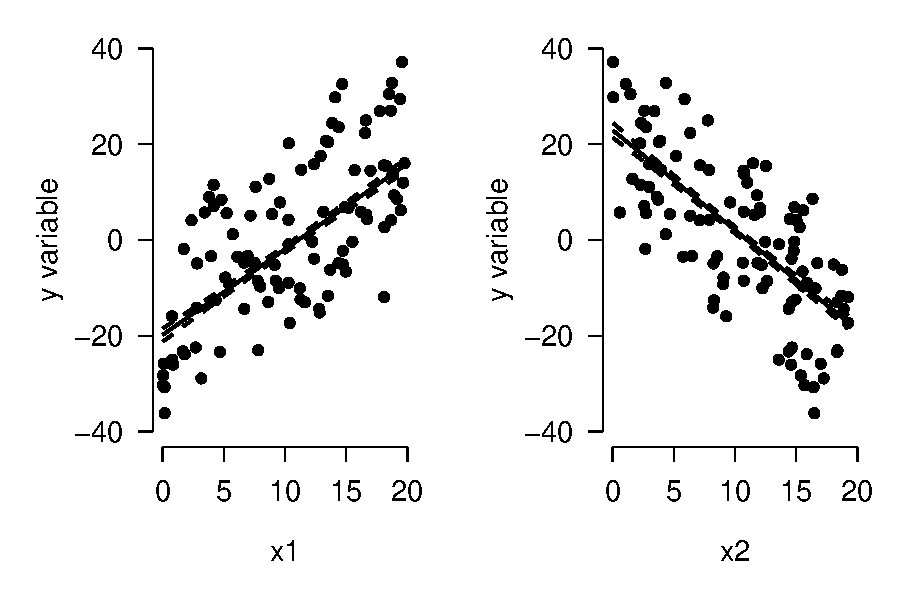
\includegraphics[keepaspectratio]{chapters/04-linear-models_files/figure-pdf/unnamed-chunk-24-1.pdf}}

\section{Analysis of covariance
(ANCOVA)}\label{analysis-of-covariance-ancova}

In \textbf{analysis of covariance (ANCOVA)}, a continuous response
variable is modeled using a continuous explanatory variable and a factor
(grouping variable). You've probably heard of ANCOVA before without
realizing it. When scientific studies are described on the news, the
reporter might say that the researchers ``controlled for'' the effects
of additional variables. That often means that the researchers used a
type of ANCOVA in their analysis.

The figure below shows two examples of what ANCOVA looks like in
practice. Both types of ANCOVA are extremely common in biology, so we'll
fit both (although, as we'll see, they can be the same model in JAGS).

\begin{figure}

\caption{\label{fig-ancova}Illustration of ANCOVA without an interaction
(different intercepts, same slope) and with an interaction (different
intercepts and slopes.)}

\centering{

\pandocbounded{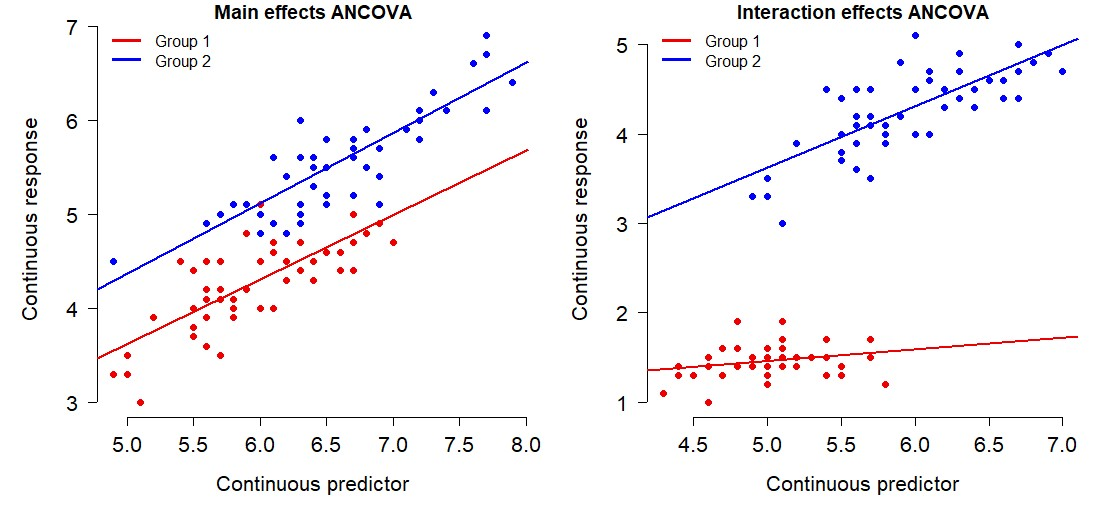
\includegraphics[keepaspectratio]{chapters/../images/06-04.jpg}}

}

\end{figure}%

\begin{itemize}
\tightlist
\item
  Left: y increases as a linear function of x, and values in group 2
  tend to be larger than values in group 1. Groups 1 and 2 share the
  same slope, so x has the same effect on y in both groups.
\item
  Right: y varies as a function of x, and the effect of x on y is
  different in each group (i.e., the slopes are different). This is
  ``interaction effects'' ANCOVA, or ``ANCOVA with interaction''. An
  ``interaction'' means that the effect of one variable affects the
  effect of another variable.
\end{itemize}

\subparagraph{figure}\label{figure}

\subsection{ANCOVA with main effects
only}\label{ancova-with-main-effects-only}

As always, we'll simulate a dataset and then analyze it. Before that we
need to think about how we want to write the ANCOVA model. The
traditional way is the effects parameterization:

\[y_i=Normal\left(\eta_i,\sigma_{res}\right)\]

\[\eta_i=\beta_0+\beta_1{x1}_i+\beta_2{x2}_i\]

where x1 is the continuous predictor variable, and x2 is a variable (or
matrix of dummy variables) that describes group membership (i.e., levels
of the factor). This model has an intercept (\(\beta_0\)) and a term
that describes group effects (\(\beta_0\)). The downside of writing the
model this way is in how effects are represented: as differences from
the baseline level. This can be confusing to add up.

Grouping the factor effects and the intercept gives us something more
like a means parameterization of ANCOVA:

\[y_i=Normal\left(\eta_i,\sigma_{res}\right)\]

\[\eta_i=\beta_{0,{fac}_i}+\beta_1{x1}_i\]

Here the \(\beta_2\) term is combined with the intercept, such that the
intercept varies between groups: \(\beta_{0,{fac}_i}\). This version of
the model avoids the awkwardness of having to add parameters together to
see what the values in each group should be.

The means parameterization of ANCOVA is easier to deal with in JAGS than
the effects parameterization, and is easy to extend to other situations,
including mixed models.

\begin{Shaded}
\begin{Highlighting}[]
\CommentTok{\# simulate some data}
\FunctionTok{set.seed}\NormalTok{(}\DecValTok{123}\NormalTok{)}
\NormalTok{n }\OtherTok{\textless{}{-}} \DecValTok{50}
\NormalTok{nfac }\OtherTok{\textless{}{-}} \DecValTok{3}
\NormalTok{dx }\OtherTok{\textless{}{-}} \FunctionTok{data.frame}\NormalTok{(}\AttributeTok{x1=}\FunctionTok{runif}\NormalTok{(n}\SpecialCharTok{*}\NormalTok{nfac, }\DecValTok{0}\NormalTok{, }\DecValTok{20}\NormalTok{),}
    \AttributeTok{fac1=}\FunctionTok{rep}\NormalTok{(}\DecValTok{1}\SpecialCharTok{:}\NormalTok{nfac, }\AttributeTok{each=}\NormalTok{n))}

\NormalTok{beta0 }\OtherTok{\textless{}{-}} \FunctionTok{c}\NormalTok{(}\SpecialCharTok{{-}}\DecValTok{10}\NormalTok{, }\DecValTok{0}\NormalTok{, }\DecValTok{10}\NormalTok{)}
\NormalTok{beta1 }\OtherTok{\textless{}{-}} \FloatTok{1.8}
\NormalTok{sigma.res }\OtherTok{\textless{}{-}} \DecValTok{3}
\NormalTok{dx}\SpecialCharTok{$}\NormalTok{y }\OtherTok{\textless{}{-}}\NormalTok{ beta0[dx}\SpecialCharTok{$}\NormalTok{fac1] }\SpecialCharTok{+}\NormalTok{ beta1}\SpecialCharTok{*}\NormalTok{dx}\SpecialCharTok{$}\NormalTok{x1 }\SpecialCharTok{+}
    \FunctionTok{rnorm}\NormalTok{(}\FunctionTok{nrow}\NormalTok{(dx), }\DecValTok{0}\NormalTok{, sigma.res)}

\NormalTok{dx}\SpecialCharTok{$}\NormalTok{col }\OtherTok{\textless{}{-}} \FunctionTok{rainbow}\NormalTok{(}\DecValTok{3}\NormalTok{)[dx}\SpecialCharTok{$}\NormalTok{fac1]}
\FunctionTok{plot}\NormalTok{(dx}\SpecialCharTok{$}\NormalTok{x1, dx}\SpecialCharTok{$}\NormalTok{y, }\AttributeTok{col=}\NormalTok{dx}\SpecialCharTok{$}\NormalTok{col)}
\end{Highlighting}
\end{Shaded}

\pandocbounded{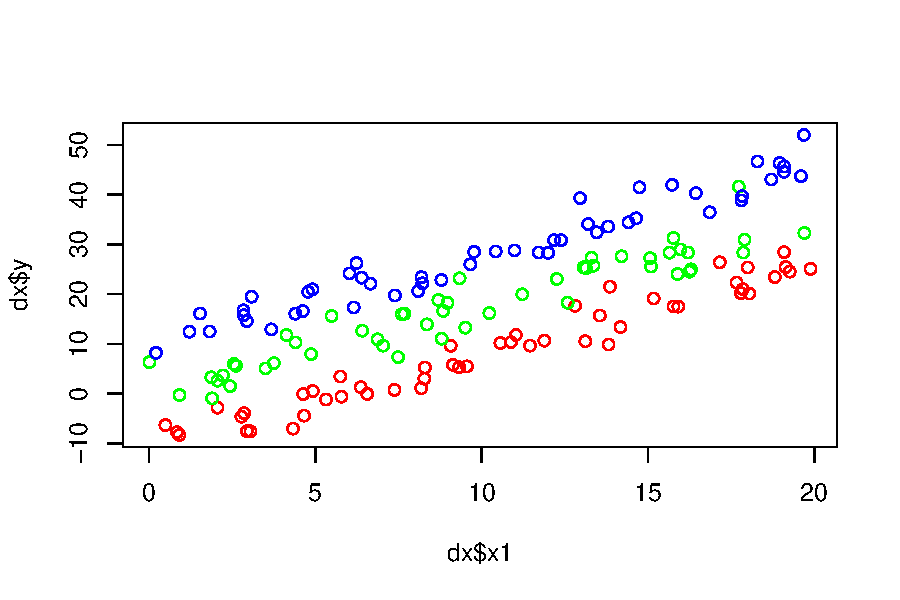
\includegraphics[keepaspectratio]{chapters/04-linear-models_files/figure-pdf/fit-ancovamain-jags-1.pdf}}

\begin{Shaded}
\begin{Highlighting}[]
\FunctionTok{summary}\NormalTok{(}\FunctionTok{lm}\NormalTok{(y}\SpecialCharTok{\textasciitilde{}}\NormalTok{x1}\SpecialCharTok{+}\FunctionTok{factor}\NormalTok{(fac1), }\AttributeTok{data=}\NormalTok{dx))}
\end{Highlighting}
\end{Shaded}

\begin{verbatim}

Call:
lm(formula = y ~ x1 + factor(fac1), data = dx)

Residuals:
    Min      1Q  Median      3Q     Max 
-6.1114 -1.8415 -0.3887  1.7631  9.6479 

Coefficients:
               Estimate Std. Error t value Pr(>|t|)    
(Intercept)   -10.11686    0.59274  -17.07   <2e-16 ***
x1              1.81207    0.04129   43.88   <2e-16 ***
factor(fac1)2   9.97812    0.57875   17.24   <2e-16 ***
factor(fac1)3  19.94729    0.57767   34.53   <2e-16 ***
---
Signif. codes:  0 '***' 0.001 '**' 0.01 '*' 0.05 '.' 0.1 ' ' 1

Residual standard error: 2.888 on 146 degrees of freedom
Multiple R-squared:  0.9551,    Adjusted R-squared:  0.9542 
F-statistic:  1035 on 3 and 146 DF,  p-value: < 2.2e-16
\end{verbatim}

\begin{Shaded}
\begin{Highlighting}[]
\CommentTok{\# linear regression with 2 predictors}
\NormalTok{mod.name }\OtherTok{\textless{}{-}} \StringTok{"jags\_ancova\_main\_1x1f.txt"}
\FunctionTok{sink}\NormalTok{(mod.name)}
\FunctionTok{cat}\NormalTok{(}\StringTok{"}
\StringTok{    model\{}
\StringTok{        \# priors}
\StringTok{        \#\# intercept}
\StringTok{        for(i in 1:nfac1)\{}
\StringTok{            beta0[i] \textasciitilde{} dnorm(0, 0.001)}
\StringTok{        \}\#i}

\StringTok{        \#\# slope}
\StringTok{        beta1 \textasciitilde{} dnorm(0, 0.001)}

\StringTok{        \#\# residual SD and precision}
\StringTok{        sigma \textasciitilde{} dlnorm(1, 0.25)}
\StringTok{        tau \textless{}{-} 1 / (sigma\^{}2)}

\StringTok{        \# likelihood}
\StringTok{        for(i in 1:n)\{}
\StringTok{            y[i] \textasciitilde{} dnorm(eta[i], tau)}
\StringTok{            eta[i] \textless{}{-} beta0[fac1[i]] + beta1 * x1[i]}
\StringTok{        \}\#i}

\StringTok{    \}\#model}

\StringTok{"}\NormalTok{, }\AttributeTok{fill=}\ConstantTok{TRUE}\NormalTok{)}
\FunctionTok{sink}\NormalTok{()}

\CommentTok{\# parameters to monitor}
\NormalTok{params }\OtherTok{\textless{}{-}} \FunctionTok{c}\NormalTok{(}\StringTok{"beta0"}\NormalTok{, }\StringTok{"beta1"}\NormalTok{, }\StringTok{"sigma"}\NormalTok{)}

\CommentTok{\# MCMC parameters}
\NormalTok{n.iter }\OtherTok{\textless{}{-}} \FloatTok{5e4}
\NormalTok{n.burnin }\OtherTok{\textless{}{-}} \FloatTok{1e4}
\NormalTok{n.thin }\OtherTok{\textless{}{-}} \DecValTok{100}
\NormalTok{nchains }\OtherTok{\textless{}{-}} \DecValTok{3}

\CommentTok{\# package data for JAGS}
\NormalTok{in.data }\OtherTok{\textless{}{-}} \FunctionTok{list}\NormalTok{(}\AttributeTok{y=}\NormalTok{dx}\SpecialCharTok{$}\NormalTok{y, }\AttributeTok{n=}\FunctionTok{nrow}\NormalTok{(dx),}
    \AttributeTok{x1=}\NormalTok{dx}\SpecialCharTok{$}\NormalTok{x1,}
    \AttributeTok{fac1=}\NormalTok{dx}\SpecialCharTok{$}\NormalTok{fac1, }\AttributeTok{nfac1=}\NormalTok{nfac)}


\CommentTok{\# function to define initial values for MCMC chains}
\NormalTok{init.fun }\OtherTok{\textless{}{-}} \ControlFlowTok{function}\NormalTok{(nc)\{}
\NormalTok{    res }\OtherTok{\textless{}{-}} \FunctionTok{vector}\NormalTok{(}\StringTok{"list"}\NormalTok{, }\AttributeTok{length=}\NormalTok{nc)}
    \ControlFlowTok{for}\NormalTok{(i }\ControlFlowTok{in} \DecValTok{1}\SpecialCharTok{:}\NormalTok{nc)\{}
\NormalTok{        res[[i]] }\OtherTok{\textless{}{-}} \FunctionTok{list}\NormalTok{(}\AttributeTok{beta0=}\FunctionTok{rnorm}\NormalTok{(nfac, }\DecValTok{0}\NormalTok{, }\DecValTok{100}\NormalTok{),}
                         \AttributeTok{beta1=}\FunctionTok{rnorm}\NormalTok{(}\DecValTok{1}\NormalTok{, }\DecValTok{0}\NormalTok{, }\DecValTok{100}\NormalTok{),}
                         \AttributeTok{sigma=}\FunctionTok{rlnorm}\NormalTok{(}\DecValTok{1}\NormalTok{, }\DecValTok{1}\NormalTok{, }\DecValTok{2}\NormalTok{))}
\NormalTok{    \}}
    \FunctionTok{return}\NormalTok{(res)}
\NormalTok{\}}
\NormalTok{inits }\OtherTok{\textless{}{-}} \FunctionTok{init.fun}\NormalTok{(nchains)}

\CommentTok{\# fit model}
\NormalTok{mod10 }\OtherTok{\textless{}{-}} \FunctionTok{jags}\NormalTok{(}\AttributeTok{data=}\NormalTok{in.data, }\AttributeTok{inits=}\NormalTok{inits,}
              \AttributeTok{parameters.to.save=}\NormalTok{params,}
              \AttributeTok{model.file=}\NormalTok{mod.name,}
              \AttributeTok{n.chains=}\NormalTok{nchains, }\AttributeTok{n.iter=}\NormalTok{n.iter,}
              \AttributeTok{n.burnin=}\NormalTok{n.burnin, }\AttributeTok{n.thin=}\NormalTok{n.thin)}\CommentTok{\#jags}
\end{Highlighting}
\end{Shaded}

\begin{verbatim}
Compiling model graph
   Resolving undeclared variables
   Allocating nodes
Graph information:
   Observed stochastic nodes: 150
   Unobserved stochastic nodes: 5
   Total graph size: 764

Initializing model
\end{verbatim}

\begin{Shaded}
\begin{Highlighting}[]
\NormalTok{mod10}
\end{Highlighting}
\end{Shaded}

\begin{verbatim}
Inference for Bugs model at "jags_ancova_main_1x1f.txt", fit using jags,
 3 chains, each with 50000 iterations (first 10000 discarded), n.thin = 100
 n.sims = 1200 iterations saved. Running time = 15.13 secs
         mu.vect sd.vect    2.5%     25%     50%     75%   97.5%  Rhat n.eff
beta0[1] -10.126   0.604 -11.292 -10.553 -10.107  -9.728  -8.898 1.002   780
beta0[2]  -0.147   0.585  -1.268  -0.556  -0.164   0.258   1.029 1.003   680
beta0[3]   9.817   0.571   8.727   9.419   9.834  10.200  10.890 1.003   700
beta1      1.813   0.041   1.725   1.787   1.813   1.839   1.895 1.002   950
sigma      2.901   0.169   2.601   2.784   2.888   3.006   3.237 1.000  1200
deviance 744.936   3.126 740.660 742.604 744.365 746.445 752.664 1.000  1200

For each parameter, n.eff is a crude measure of effective sample size,
and Rhat is the potential scale reduction factor (at convergence, Rhat=1).

DIC info (using the rule: pV = var(deviance)/2)
pV = 4.9 and DIC = 749.8
DIC is an estimate of expected predictive error (lower deviance is better).
\end{verbatim}

The estimated slope and group-level means are basically correct, up to
sampling error.

\subsubsection{Plotting ANCOVA with main effects
only}\label{plotting-ancova-with-main-effects-only}

Making a plot with predictions and their 95\% CRI is similar to what we
did for multiple linear regression. We need to generate predictions
within each group of the factor \texttt{fac1} using the group-specific
parameters, and present the groups with different colors, symbols, line
styles, etc.

\begin{Shaded}
\begin{Highlighting}[]
\CommentTok{\# matrix of coefficients}
\NormalTok{prx }\OtherTok{\textless{}{-}}\NormalTok{ mod10}\SpecialCharTok{$}\NormalTok{BUGSoutput}\SpecialCharTok{$}\NormalTok{sims.matrix}
\DocumentationTok{\#\# don\textquotesingle{}t need deviance or sigma}
\NormalTok{prx }\OtherTok{\textless{}{-}}\NormalTok{ prx[,}\FunctionTok{grep}\NormalTok{(}\StringTok{"beta"}\NormalTok{, }\FunctionTok{colnames}\NormalTok{(prx))]}

\CommentTok{\# x values at which to predict}
\NormalTok{pred.n }\OtherTok{\textless{}{-}} \DecValTok{100}
\NormalTok{px }\OtherTok{\textless{}{-}} \FunctionTok{seq}\NormalTok{(}\FunctionTok{min}\NormalTok{(dx}\SpecialCharTok{$}\NormalTok{x1), }\FunctionTok{max}\NormalTok{(dx}\SpecialCharTok{$}\NormalTok{x1), }\AttributeTok{length=}\NormalTok{pred.n)}

\CommentTok{\# set up matrices for predictions}
\CommentTok{\# one for each group (level of fac1)}
\NormalTok{preddf }\OtherTok{\textless{}{-}} \FunctionTok{expand.grid}\NormalTok{(}\AttributeTok{x1=}\NormalTok{px, }\AttributeTok{fac1=}\DecValTok{1}\SpecialCharTok{:}\NormalTok{nfac)}
\NormalTok{npred }\OtherTok{\textless{}{-}} \FunctionTok{nrow}\NormalTok{(preddf)}

\NormalTok{pred }\OtherTok{\textless{}{-}} \FunctionTok{matrix}\NormalTok{(}\ConstantTok{NA}\NormalTok{, }\AttributeTok{nrow=}\FunctionTok{nrow}\NormalTok{(preddf), }\AttributeTok{ncol=}\NormalTok{post.n)}

\CommentTok{\# fill in a loop}
\ControlFlowTok{for}\NormalTok{(i }\ControlFlowTok{in} \DecValTok{1}\SpecialCharTok{:}\NormalTok{post.n)\{}
\NormalTok{    pred[,i] }\OtherTok{\textless{}{-}}\NormalTok{ prx[i,preddf}\SpecialCharTok{$}\NormalTok{fac1] }\SpecialCharTok{+}
\NormalTok{        prx[i,}\StringTok{"beta1"}\NormalTok{] }\SpecialCharTok{*}\NormalTok{ preddf}\SpecialCharTok{$}\NormalTok{x1}
\NormalTok{\}}\CommentTok{\#i}

\CommentTok{\# apply to get mean and CRI}
\NormalTok{preddf}\SpecialCharTok{$}\NormalTok{mn }\OtherTok{\textless{}{-}} \FunctionTok{apply}\NormalTok{(pred, }\DecValTok{1}\NormalTok{, mean)}
\NormalTok{preddf}\SpecialCharTok{$}\NormalTok{lo }\OtherTok{\textless{}{-}} \FunctionTok{apply}\NormalTok{(pred, }\DecValTok{1}\NormalTok{, quantile, }\FloatTok{0.025}\NormalTok{)}
\NormalTok{preddf}\SpecialCharTok{$}\NormalTok{up }\OtherTok{\textless{}{-}} \FunctionTok{apply}\NormalTok{(pred, }\DecValTok{1}\NormalTok{, quantile, }\FloatTok{0.975}\NormalTok{)}

\CommentTok{\# define some colors and shapes:}
\NormalTok{cols }\OtherTok{\textless{}{-}} \FunctionTok{rainbow}\NormalTok{(nfac)}
\NormalTok{pchs }\OtherTok{\textless{}{-}} \DecValTok{15}\SpecialCharTok{:}\DecValTok{17} \CommentTok{\# square, circle, triangle}

\CommentTok{\# fancy plot options with par()}
\FunctionTok{par}\NormalTok{(}\AttributeTok{mfrow=}\FunctionTok{c}\NormalTok{(}\DecValTok{1}\NormalTok{,}\DecValTok{1}\NormalTok{), }\AttributeTok{mar=}\FunctionTok{c}\NormalTok{(}\FloatTok{5.1}\NormalTok{, }\FloatTok{5.1}\NormalTok{, }\FloatTok{1.1}\NormalTok{, }\FloatTok{1.1}\NormalTok{),}
    \AttributeTok{bty=}\StringTok{"n"}\NormalTok{, }\AttributeTok{lend=}\DecValTok{1}\NormalTok{,}
    \AttributeTok{las=}\DecValTok{1}\NormalTok{, }\AttributeTok{cex.axis=}\FloatTok{1.2}\NormalTok{, }\AttributeTok{cex.lab=}\FloatTok{1.2}\NormalTok{)}
\CommentTok{\# x1 plot}
\FunctionTok{plot}\NormalTok{(dx}\SpecialCharTok{$}\NormalTok{x1, dx}\SpecialCharTok{$}\NormalTok{y, }\AttributeTok{type=}\StringTok{"n"}\NormalTok{,}
    \AttributeTok{ylim=}\FunctionTok{c}\NormalTok{(}\SpecialCharTok{{-}}\DecValTok{10}\NormalTok{, }\DecValTok{50}\NormalTok{), }\AttributeTok{xlim=}\FunctionTok{c}\NormalTok{(}\DecValTok{0}\NormalTok{, }\DecValTok{20}\NormalTok{),}
    \AttributeTok{xlab=}\StringTok{"x1"}\NormalTok{, }\AttributeTok{ylab=}\StringTok{"y"}\NormalTok{)}
\ControlFlowTok{for}\NormalTok{(i }\ControlFlowTok{in} \DecValTok{1}\SpecialCharTok{:}\NormalTok{nfac)\{}
\NormalTok{    flag }\OtherTok{\textless{}{-}} \FunctionTok{which}\NormalTok{(preddf}\SpecialCharTok{$}\NormalTok{fac1}\SpecialCharTok{==}\NormalTok{i)}
    \FunctionTok{points}\NormalTok{(px, preddf}\SpecialCharTok{$}\NormalTok{mn[flag], }\AttributeTok{type=}\StringTok{"l"}\NormalTok{,}
        \AttributeTok{lwd=}\DecValTok{3}\NormalTok{, }\AttributeTok{col=}\NormalTok{cols[i])}
    \FunctionTok{points}\NormalTok{(px, preddf}\SpecialCharTok{$}\NormalTok{lo[flag], }\AttributeTok{type=}\StringTok{"l"}\NormalTok{,}
        \AttributeTok{lwd=}\DecValTok{3}\NormalTok{, }\AttributeTok{lty=}\DecValTok{2}\NormalTok{, }\AttributeTok{col=}\NormalTok{cols[i])}
    \FunctionTok{points}\NormalTok{(px, preddf}\SpecialCharTok{$}\NormalTok{up[flag], }\AttributeTok{type=}\StringTok{"l"}\NormalTok{,}
        \AttributeTok{lwd=}\DecValTok{3}\NormalTok{, }\AttributeTok{lty=}\DecValTok{2}\NormalTok{, }\AttributeTok{col=}\NormalTok{cols[i])}
\NormalTok{\}}\CommentTok{\#i}
\CommentTok{\# put original data on top, so not covered by }
\CommentTok{\# lines and etc.}
\FunctionTok{points}\NormalTok{(dx}\SpecialCharTok{$}\NormalTok{x1, dx}\SpecialCharTok{$}\NormalTok{y, }\AttributeTok{pch=}\NormalTok{pchs[dx}\SpecialCharTok{$}\NormalTok{fac1], }\AttributeTok{col=}\NormalTok{cols[dx}\SpecialCharTok{$}\NormalTok{fac1])}
\FunctionTok{legend}\NormalTok{(}\StringTok{"topleft"}\NormalTok{, }\AttributeTok{legend=}\FunctionTok{paste}\NormalTok{(}\StringTok{"Group"}\NormalTok{, }\DecValTok{1}\SpecialCharTok{:}\NormalTok{nfac),}
       \AttributeTok{pch=}\NormalTok{pchs, }\AttributeTok{col=}\NormalTok{cols, }\AttributeTok{cex=}\FloatTok{1.2}\NormalTok{)}
\end{Highlighting}
\end{Shaded}

\pandocbounded{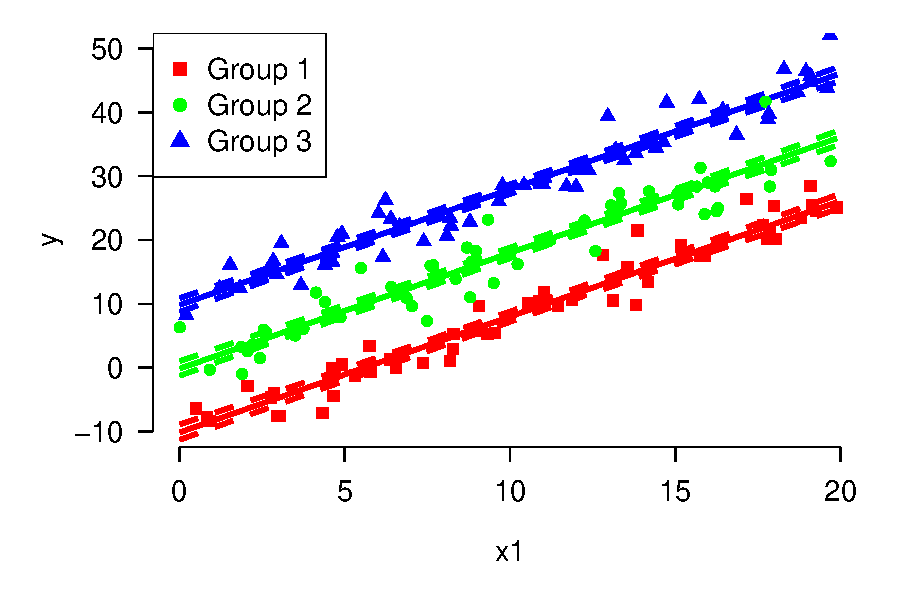
\includegraphics[keepaspectratio]{chapters/04-linear-models_files/figure-pdf/unnamed-chunk-25-1.pdf}}

\subsection{ANCOVA with interaction}\label{ancova-with-interaction}

The ANCOVA with interaction effect model will be constructed by
combining bits of the main effects ANCOVA model with the ``parameters as
arrays'' trick we learned in the ANOVA with interaction model. The key
is that each group has its own slope and intercept.

\begin{Shaded}
\begin{Highlighting}[]
\CommentTok{\# simulate some data}
\FunctionTok{set.seed}\NormalTok{(}\DecValTok{123}\NormalTok{)}
\NormalTok{n }\OtherTok{\textless{}{-}} \DecValTok{100}
\NormalTok{nfac }\OtherTok{\textless{}{-}} \DecValTok{3}
\NormalTok{dx }\OtherTok{\textless{}{-}} \FunctionTok{data.frame}\NormalTok{(}\AttributeTok{x1=}\FunctionTok{runif}\NormalTok{(n}\SpecialCharTok{*}\NormalTok{nfac, }\DecValTok{0}\NormalTok{, }\DecValTok{20}\NormalTok{),}
    \AttributeTok{fac1=}\FunctionTok{rep}\NormalTok{(}\DecValTok{1}\SpecialCharTok{:}\NormalTok{nfac, }\AttributeTok{each=}\NormalTok{n))}

\NormalTok{beta0 }\OtherTok{\textless{}{-}} \FunctionTok{c}\NormalTok{(}\DecValTok{5}\NormalTok{, }\DecValTok{10}\NormalTok{, }\DecValTok{15}\NormalTok{)}
\NormalTok{beta1 }\OtherTok{\textless{}{-}} \FunctionTok{c}\NormalTok{(}\FloatTok{0.8}\NormalTok{, }\FloatTok{2.5}\NormalTok{, }\SpecialCharTok{{-}}\FloatTok{1.6}\NormalTok{)}
\NormalTok{sigma.res }\OtherTok{\textless{}{-}} \DecValTok{3}
\NormalTok{dx}\SpecialCharTok{$}\NormalTok{y }\OtherTok{\textless{}{-}}\NormalTok{ beta0[dx}\SpecialCharTok{$}\NormalTok{fac1] }\SpecialCharTok{+}\NormalTok{ beta1[dx}\SpecialCharTok{$}\NormalTok{fac1]}\SpecialCharTok{*}\NormalTok{dx}\SpecialCharTok{$}\NormalTok{x1 }\SpecialCharTok{+}
    \FunctionTok{rnorm}\NormalTok{(}\FunctionTok{nrow}\NormalTok{(dx), }\DecValTok{0}\NormalTok{, sigma.res)}

\NormalTok{dx}\SpecialCharTok{$}\NormalTok{col }\OtherTok{\textless{}{-}} \FunctionTok{rainbow}\NormalTok{(}\DecValTok{3}\NormalTok{)[dx}\SpecialCharTok{$}\NormalTok{fac1]}
\FunctionTok{plot}\NormalTok{(dx}\SpecialCharTok{$}\NormalTok{x1, dx}\SpecialCharTok{$}\NormalTok{y, }\AttributeTok{col=}\NormalTok{dx}\SpecialCharTok{$}\NormalTok{col)}
\end{Highlighting}
\end{Shaded}

\pandocbounded{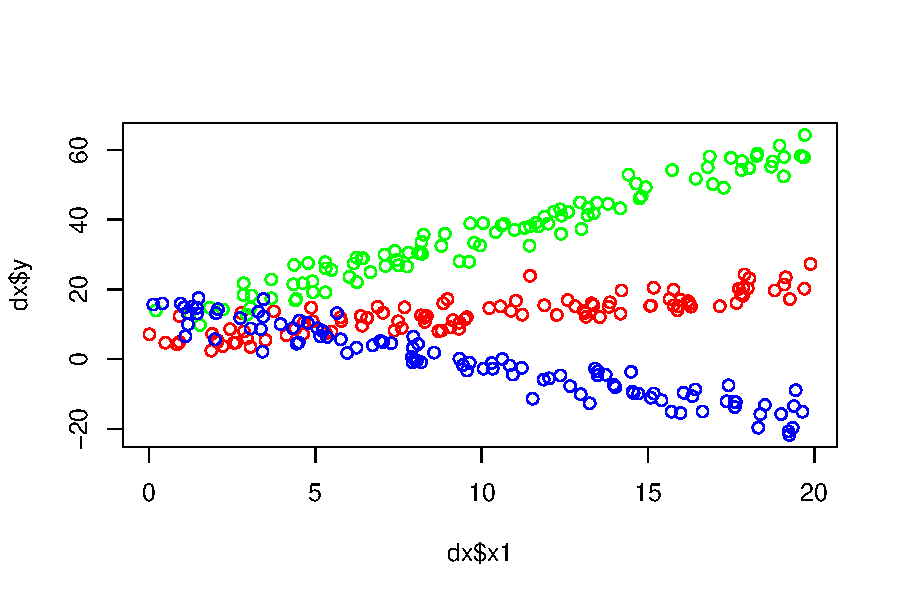
\includegraphics[keepaspectratio]{chapters/04-linear-models_files/figure-pdf/fit-ancovainter-jags-1.pdf}}

\begin{Shaded}
\begin{Highlighting}[]
\FunctionTok{summary}\NormalTok{(}\FunctionTok{lm}\NormalTok{(y}\SpecialCharTok{\textasciitilde{}}\NormalTok{x1}\SpecialCharTok{*}\FunctionTok{factor}\NormalTok{(fac1), }\AttributeTok{data=}\NormalTok{dx))}
\end{Highlighting}
\end{Shaded}

\begin{verbatim}

Call:
lm(formula = y ~ x1 * factor(fac1), data = dx)

Residuals:
    Min      1Q  Median      3Q     Max 
-7.6183 -1.9110 -0.0861  1.7883  9.7024 

Coefficients:
                 Estimate Std. Error t value Pr(>|t|)    
(Intercept)       5.21178    0.60045   8.680 2.77e-16 ***
x1                0.78332    0.05234  14.965  < 2e-16 ***
factor(fac1)2     4.82355    0.88711   5.437 1.14e-07 ***
factor(fac1)3    10.24185    0.83151  12.317  < 2e-16 ***
x1:factor(fac1)2  1.74993    0.07706  22.708  < 2e-16 ***
x1:factor(fac1)3 -2.45160    0.07286 -33.648  < 2e-16 ***
---
Signif. codes:  0 '***' 0.001 '**' 0.01 '*' 0.05 '.' 0.1 ' ' 1

Residual standard error: 2.969 on 294 degrees of freedom
Multiple R-squared:  0.9744,    Adjusted R-squared:  0.9739 
F-statistic:  2236 on 5 and 294 DF,  p-value: < 2.2e-16
\end{verbatim}

\begin{Shaded}
\begin{Highlighting}[]
\CommentTok{\# linear regression with 2 predictors}
\NormalTok{mod.name }\OtherTok{\textless{}{-}} \StringTok{"jags\_ancova\_inter\_1x1f.txt"}
\FunctionTok{sink}\NormalTok{(mod.name)}
\FunctionTok{cat}\NormalTok{(}\StringTok{"}
\StringTok{    model\{}
\StringTok{        \# priors}
\StringTok{        \#\# intercept and slope}
\StringTok{        for(i in 1:nfac1)\{}
\StringTok{            beta0[i] \textasciitilde{} dnorm(0, 0.001)}
\StringTok{            beta1[i] \textasciitilde{} dnorm(0, 0.001)}
\StringTok{        \}\#i}

\StringTok{        \#\# residual SD and precision}
\StringTok{        sigma \textasciitilde{} dlnorm(1, 0.25)}
\StringTok{        tau \textless{}{-} 1 / (sigma\^{}2)}

\StringTok{        \# likelihood}
\StringTok{        for(i in 1:n)\{}
\StringTok{            y[i] \textasciitilde{} dnorm(eta[i], tau)}
\StringTok{            eta[i] \textless{}{-} beta0[fac1[i]] + beta1[fac1[i]] * x1[i]}
\StringTok{        \}\#i}

\StringTok{    \}\#model}

\StringTok{"}\NormalTok{, }\AttributeTok{fill=}\ConstantTok{TRUE}\NormalTok{)}
\FunctionTok{sink}\NormalTok{()}

\CommentTok{\# parameters to monitor}
\NormalTok{params }\OtherTok{\textless{}{-}} \FunctionTok{c}\NormalTok{(}\StringTok{"beta0"}\NormalTok{, }\StringTok{"beta1"}\NormalTok{, }\StringTok{"sigma"}\NormalTok{)}

\CommentTok{\# MCMC parameters}
\NormalTok{n.iter }\OtherTok{\textless{}{-}} \FloatTok{5e4}
\NormalTok{n.burnin }\OtherTok{\textless{}{-}} \FloatTok{1e4}
\NormalTok{n.thin }\OtherTok{\textless{}{-}} \DecValTok{100}
\NormalTok{nchains }\OtherTok{\textless{}{-}} \DecValTok{3}

\CommentTok{\# package data for JAGS}
\NormalTok{in.data }\OtherTok{\textless{}{-}} \FunctionTok{list}\NormalTok{(}\AttributeTok{y=}\NormalTok{dx}\SpecialCharTok{$}\NormalTok{y, }\AttributeTok{n=}\FunctionTok{nrow}\NormalTok{(dx),}
    \AttributeTok{x1=}\NormalTok{dx}\SpecialCharTok{$}\NormalTok{x1,}
    \AttributeTok{fac1=}\NormalTok{dx}\SpecialCharTok{$}\NormalTok{fac1, }\AttributeTok{nfac1=}\NormalTok{nfac)}


\CommentTok{\# function to define initial values for MCMC chains}
\NormalTok{init.fun }\OtherTok{\textless{}{-}} \ControlFlowTok{function}\NormalTok{(nc)\{}
\NormalTok{    res }\OtherTok{\textless{}{-}} \FunctionTok{vector}\NormalTok{(}\StringTok{"list"}\NormalTok{, }\AttributeTok{length=}\NormalTok{nc)}
    \ControlFlowTok{for}\NormalTok{(i }\ControlFlowTok{in} \DecValTok{1}\SpecialCharTok{:}\NormalTok{nc)\{}
\NormalTok{        res[[i]] }\OtherTok{\textless{}{-}} \FunctionTok{list}\NormalTok{(}\AttributeTok{beta0=}\FunctionTok{rnorm}\NormalTok{(nfac, }\DecValTok{0}\NormalTok{, }\DecValTok{100}\NormalTok{),}
                         \AttributeTok{beta1=}\FunctionTok{rnorm}\NormalTok{(nfac, }\DecValTok{0}\NormalTok{, }\DecValTok{100}\NormalTok{),}
                         \AttributeTok{sigma=}\FunctionTok{rlnorm}\NormalTok{(}\DecValTok{1}\NormalTok{, }\DecValTok{1}\NormalTok{, }\DecValTok{2}\NormalTok{))}
\NormalTok{    \}}
    \FunctionTok{return}\NormalTok{(res)}
\NormalTok{\}}
\NormalTok{inits }\OtherTok{\textless{}{-}} \FunctionTok{init.fun}\NormalTok{(nchains)}

\CommentTok{\# fit model}
\NormalTok{mod11 }\OtherTok{\textless{}{-}} \FunctionTok{jags}\NormalTok{(}\AttributeTok{data=}\NormalTok{in.data, }\AttributeTok{inits=}\NormalTok{inits,}
              \AttributeTok{parameters.to.save=}\NormalTok{params,}
              \AttributeTok{model.file=}\NormalTok{mod.name,}
              \AttributeTok{n.chains=}\NormalTok{nchains, }\AttributeTok{n.iter=}\NormalTok{n.iter,}
              \AttributeTok{n.burnin=}\NormalTok{n.burnin, }\AttributeTok{n.thin=}\NormalTok{n.thin)}\CommentTok{\#jags}
\end{Highlighting}
\end{Shaded}

\begin{verbatim}
Compiling model graph
   Resolving undeclared variables
   Allocating nodes
Graph information:
   Observed stochastic nodes: 300
   Unobserved stochastic nodes: 7
   Total graph size: 1516

Initializing model
\end{verbatim}

\begin{Shaded}
\begin{Highlighting}[]
\NormalTok{mod11}
\end{Highlighting}
\end{Shaded}

\begin{verbatim}
Inference for Bugs model at "jags_ancova_inter_1x1f.txt", fit using jags,
 3 chains, each with 50000 iterations (first 10000 discarded), n.thin = 100
 n.sims = 1200 iterations saved. Running time = 29.86 secs
          mu.vect sd.vect     2.5%      25%      50%      75%    97.5%  Rhat
beta0[1]    5.203   0.639    3.968    4.747    5.203    5.634    6.451 1.001
beta0[2]   10.045   0.670    8.731    9.600   10.033   10.485   11.448 1.002
beta0[3]   15.428   0.581   14.323   15.050   15.425   15.844   16.502 1.003
beta1[1]    0.783   0.055    0.677    0.745    0.784    0.823    0.887 1.000
beta1[2]    2.532   0.057    2.424    2.493    2.532    2.567    2.647 1.003
beta1[3]   -1.667   0.051   -1.764   -1.702   -1.668   -1.632   -1.567 1.006
sigma       2.972   0.124    2.735    2.886    2.969    3.052    3.227 1.001
deviance 1505.402   3.887 1500.017 1502.500 1504.658 1507.450 1514.401 1.000
         n.eff
beta0[1]  1200
beta0[2]  1200
beta0[3]   830
beta1[1]  1200
beta1[2]   990
beta1[3]   300
sigma     1200
deviance  1200

For each parameter, n.eff is a crude measure of effective sample size,
and Rhat is the potential scale reduction factor (at convergence, Rhat=1).

DIC info (using the rule: pV = var(deviance)/2)
pV = 7.6 and DIC = 1513.0
DIC is an estimate of expected predictive error (lower deviance is better).
\end{verbatim}

\subsubsection{Plotting ANCOVA with
interactions}\label{plotting-ancova-with-interactions}

And the plot, much as for the ANCOVA without interactions:

\begin{Shaded}
\begin{Highlighting}[]
\CommentTok{\# matrix of coefficients}
\NormalTok{prx }\OtherTok{\textless{}{-}}\NormalTok{ mod11}\SpecialCharTok{$}\NormalTok{BUGSoutput}\SpecialCharTok{$}\NormalTok{sims.matrix}
\DocumentationTok{\#\# don\textquotesingle{}t need deviance or sigma}
\NormalTok{prx }\OtherTok{\textless{}{-}}\NormalTok{ prx[,}\FunctionTok{grep}\NormalTok{(}\StringTok{"beta"}\NormalTok{, }\FunctionTok{colnames}\NormalTok{(prx))]}

\CommentTok{\# x values at which to predict}
\NormalTok{pred.n }\OtherTok{\textless{}{-}} \DecValTok{100}
\NormalTok{px }\OtherTok{\textless{}{-}} \FunctionTok{seq}\NormalTok{(}\FunctionTok{min}\NormalTok{(dx}\SpecialCharTok{$}\NormalTok{x1), }\FunctionTok{max}\NormalTok{(dx}\SpecialCharTok{$}\NormalTok{x1), }\AttributeTok{length=}\NormalTok{pred.n)}

\CommentTok{\# set up matrices for predictions}
\CommentTok{\# one for each group (level of fac1)}
\NormalTok{preddf }\OtherTok{\textless{}{-}} \FunctionTok{expand.grid}\NormalTok{(}\AttributeTok{x1=}\NormalTok{px, }\AttributeTok{fac1=}\DecValTok{1}\SpecialCharTok{:}\NormalTok{nfac)}
\NormalTok{npred }\OtherTok{\textless{}{-}} \FunctionTok{nrow}\NormalTok{(preddf)}

\NormalTok{pred }\OtherTok{\textless{}{-}} \FunctionTok{matrix}\NormalTok{(}\ConstantTok{NA}\NormalTok{, }\AttributeTok{nrow=}\FunctionTok{nrow}\NormalTok{(preddf), }\AttributeTok{ncol=}\NormalTok{post.n)}

\CommentTok{\# fill in a loop}
\ControlFlowTok{for}\NormalTok{(i }\ControlFlowTok{in} \DecValTok{1}\SpecialCharTok{:}\NormalTok{post.n)\{}
\NormalTok{    pred[,i] }\OtherTok{\textless{}{-}}\NormalTok{ prx[i,}\FunctionTok{grep}\NormalTok{(}\StringTok{"beta0"}\NormalTok{, }\FunctionTok{colnames}\NormalTok{(prx))[preddf}\SpecialCharTok{$}\NormalTok{fac1]] }\SpecialCharTok{+}
\NormalTok{        prx[i,}\FunctionTok{grep}\NormalTok{(}\StringTok{"beta1"}\NormalTok{, }\FunctionTok{colnames}\NormalTok{(prx))[preddf}\SpecialCharTok{$}\NormalTok{fac1]] }\SpecialCharTok{*}\NormalTok{ preddf}\SpecialCharTok{$}\NormalTok{x1}
\NormalTok{\}}\CommentTok{\#i}

\CommentTok{\# apply to get mean and CRI}
\NormalTok{preddf}\SpecialCharTok{$}\NormalTok{mn }\OtherTok{\textless{}{-}} \FunctionTok{apply}\NormalTok{(pred, }\DecValTok{1}\NormalTok{, mean)}
\NormalTok{preddf}\SpecialCharTok{$}\NormalTok{lo }\OtherTok{\textless{}{-}} \FunctionTok{apply}\NormalTok{(pred, }\DecValTok{1}\NormalTok{, quantile, }\FloatTok{0.025}\NormalTok{)}
\NormalTok{preddf}\SpecialCharTok{$}\NormalTok{up }\OtherTok{\textless{}{-}} \FunctionTok{apply}\NormalTok{(pred, }\DecValTok{1}\NormalTok{, quantile, }\FloatTok{0.975}\NormalTok{)}
\CommentTok{\# define some colors and shapes:}
\NormalTok{cols }\OtherTok{\textless{}{-}} \FunctionTok{rainbow}\NormalTok{(nfac)}
\NormalTok{pchs }\OtherTok{\textless{}{-}} \DecValTok{15}\SpecialCharTok{:}\DecValTok{17} \CommentTok{\# square, circle, triangle}

\CommentTok{\# fancy plot options with par()}
\FunctionTok{par}\NormalTok{(}\AttributeTok{mfrow=}\FunctionTok{c}\NormalTok{(}\DecValTok{1}\NormalTok{,}\DecValTok{1}\NormalTok{), }\AttributeTok{mar=}\FunctionTok{c}\NormalTok{(}\FloatTok{5.1}\NormalTok{, }\FloatTok{5.1}\NormalTok{, }\FloatTok{1.1}\NormalTok{, }\FloatTok{1.1}\NormalTok{),}
    \AttributeTok{bty=}\StringTok{"n"}\NormalTok{, }\AttributeTok{lend=}\DecValTok{1}\NormalTok{,}
    \AttributeTok{las=}\DecValTok{1}\NormalTok{, }\AttributeTok{cex.axis=}\FloatTok{1.2}\NormalTok{, }\AttributeTok{cex.lab=}\FloatTok{1.2}\NormalTok{)}
\FunctionTok{plot}\NormalTok{(dx}\SpecialCharTok{$}\NormalTok{x1, dx}\SpecialCharTok{$}\NormalTok{y, }\AttributeTok{type=}\StringTok{"n"}\NormalTok{,}
    \AttributeTok{ylim=}\FunctionTok{c}\NormalTok{(}\SpecialCharTok{{-}}\DecValTok{25}\NormalTok{, }\DecValTok{75}\NormalTok{), }\AttributeTok{xlim=}\FunctionTok{c}\NormalTok{(}\DecValTok{0}\NormalTok{, }\DecValTok{20}\NormalTok{),}
    \AttributeTok{xlab=}\StringTok{"x1"}\NormalTok{, }\AttributeTok{ylab=}\StringTok{"y"}\NormalTok{)}
\ControlFlowTok{for}\NormalTok{(i }\ControlFlowTok{in} \DecValTok{1}\SpecialCharTok{:}\NormalTok{nfac)\{}
\NormalTok{    flag }\OtherTok{\textless{}{-}} \FunctionTok{which}\NormalTok{(preddf}\SpecialCharTok{$}\NormalTok{fac1}\SpecialCharTok{==}\NormalTok{i)}
    \FunctionTok{points}\NormalTok{(px, preddf}\SpecialCharTok{$}\NormalTok{mn[flag], }\AttributeTok{type=}\StringTok{"l"}\NormalTok{,}
        \AttributeTok{lwd=}\DecValTok{3}\NormalTok{, }\AttributeTok{col=}\NormalTok{cols[i])}
    \FunctionTok{points}\NormalTok{(px, preddf}\SpecialCharTok{$}\NormalTok{lo[flag], }\AttributeTok{type=}\StringTok{"l"}\NormalTok{,}
        \AttributeTok{lwd=}\DecValTok{3}\NormalTok{, }\AttributeTok{lty=}\DecValTok{2}\NormalTok{, }\AttributeTok{col=}\NormalTok{cols[i])}
    \FunctionTok{points}\NormalTok{(px, preddf}\SpecialCharTok{$}\NormalTok{up[flag], }\AttributeTok{type=}\StringTok{"l"}\NormalTok{,}
        \AttributeTok{lwd=}\DecValTok{3}\NormalTok{, }\AttributeTok{lty=}\DecValTok{2}\NormalTok{, }\AttributeTok{col=}\NormalTok{cols[i])}
\NormalTok{\}}\CommentTok{\#i}
\CommentTok{\# put original data on top, so not covered by }
\CommentTok{\# lines and etc.}
\FunctionTok{points}\NormalTok{(dx}\SpecialCharTok{$}\NormalTok{x1, dx}\SpecialCharTok{$}\NormalTok{y, }\AttributeTok{pch=}\NormalTok{pchs[dx}\SpecialCharTok{$}\NormalTok{fac1], }\AttributeTok{col=}\NormalTok{cols[dx}\SpecialCharTok{$}\NormalTok{fac1])}
\FunctionTok{legend}\NormalTok{(}\StringTok{"topleft"}\NormalTok{, }\AttributeTok{legend=}\FunctionTok{paste}\NormalTok{(}\StringTok{"Group"}\NormalTok{, }\DecValTok{1}\SpecialCharTok{:}\NormalTok{nfac),}
    \AttributeTok{pch=}\NormalTok{pchs, }\AttributeTok{col=}\NormalTok{cols, }\AttributeTok{cex=}\FloatTok{1.2}\NormalTok{)}
\end{Highlighting}
\end{Shaded}

\pandocbounded{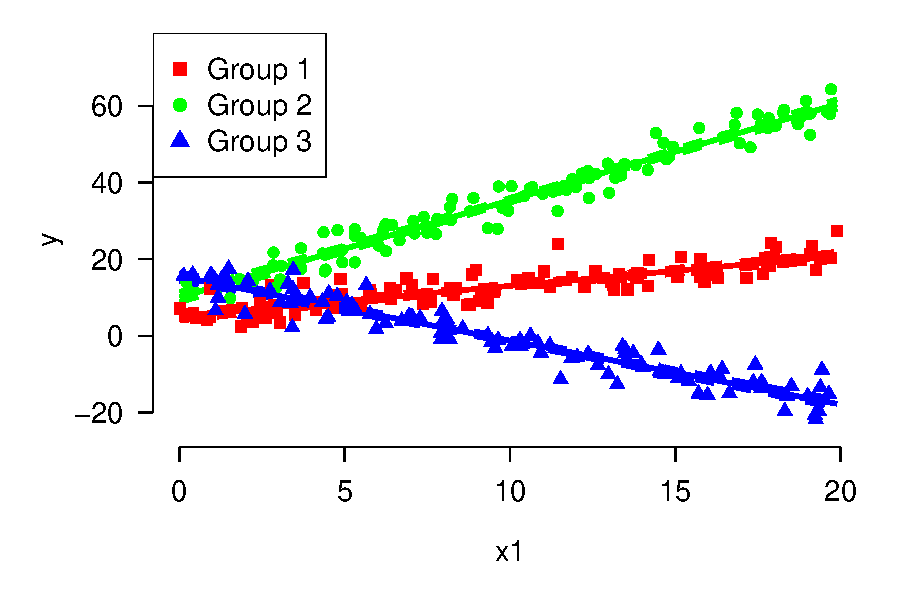
\includegraphics[keepaspectratio]{chapters/04-linear-models_files/figure-pdf/unnamed-chunk-26-1.pdf}}

\section{Linear with extra steps}\label{linear-with-extra-steps}

Earlier we discussed how some nonlinear curves can be fit statistically
as linear models, by transforming or otherwise rewriting them. I like to
think of these as ``linear with extra steps''.

\subsection{Log-linear models}\label{log-linear-models}

Log-linear models are essentially linear models where the logarithm of
the response variable is a linear function of the predictors. In other
words, it's a linear model where the response is \(log\left(y\right)\).
For this reason, the response variable in a log-linear model is strictly
positive (\(y >0\)) because \(e^a\) is positive for any real number
\(a\).

In state-space notation:

\[y_i\sim Lognormal\left(\eta_i,\ \sigma_{res}\right)\]

\[\eta_i=\beta_0+\beta_1x_i\]

Or sometimes:

\[\log{\left(y_i\right)}\sim Normal\left(\eta_i,\ \sigma_{res}\right)\]

\[\eta_i=\beta_0+\beta_1x_i\] Or even:

\[y_i\sim e^{Normal\left(\eta_i,\ \sigma_{res}\right)}\]

\[\eta_i=\beta_0+\beta_1x_i\]

No matter how you write it, the log-linear model has the deterministic
part on the log scale, and the response variable on the non-logarithmic
data scale. This means that either y follows a lognormal distribution,
or the logarithm of y follows a normal distribution. These statements
are equivalent. You can code a log-linear model either way you want in
JAGS.

\subsubsection{\texorpdfstring{Method 1: \emph{y} follows lognormal
distribution}{Method 1: y follows lognormal distribution}}\label{method-1-y-follows-lognormal-distribution}

Let's simulate some data. Notice that x and y are both on the linear
scale (not logarithmic). The x domain and model parameters were chosen
with the fact that they would be exponentiated in mind.

\begin{Shaded}
\begin{Highlighting}[]
\CommentTok{\# simulate some data}
\FunctionTok{set.seed}\NormalTok{(}\DecValTok{74656}\NormalTok{)}
\NormalTok{n }\OtherTok{\textless{}{-}} \DecValTok{40}
\NormalTok{dx }\OtherTok{\textless{}{-}} \FunctionTok{data.frame}\NormalTok{(}\AttributeTok{x=}\FunctionTok{runif}\NormalTok{(n, }\DecValTok{0}\NormalTok{, }\DecValTok{5}\NormalTok{))}

\NormalTok{beta0 }\OtherTok{\textless{}{-}} \FloatTok{0.5}
\NormalTok{beta1 }\OtherTok{\textless{}{-}} \FloatTok{1.02}
\NormalTok{sigma.res }\OtherTok{\textless{}{-}} \FloatTok{0.3}
\NormalTok{dx}\SpecialCharTok{$}\NormalTok{y }\OtherTok{\textless{}{-}} \FunctionTok{exp}\NormalTok{(beta0 }\SpecialCharTok{+}\NormalTok{ beta1}\SpecialCharTok{*}\NormalTok{dx}\SpecialCharTok{$}\NormalTok{x }\SpecialCharTok{+} \FunctionTok{rnorm}\NormalTok{(n, }\DecValTok{0}\NormalTok{, sigma.res))}

\CommentTok{\# log{-}linear model}
\NormalTok{mod.name }\OtherTok{\textless{}{-}} \StringTok{"jags\_loglinear.txt"}
\FunctionTok{sink}\NormalTok{(mod.name)}
\FunctionTok{cat}\NormalTok{(}\StringTok{"}
\StringTok{    model\{}
\StringTok{        \# priors}
\StringTok{        \#\# intercept}
\StringTok{        beta0 \textasciitilde{} dnorm(0, 0.001)}
\StringTok{        beta1 \textasciitilde{} dnorm(0, 0.001)}

\StringTok{        \#\# residual SD and precision}
\StringTok{        sigma \textasciitilde{} dlnorm(1, 0.25)}
\StringTok{        tau \textless{}{-} 1 / (sigma\^{}2)}

\StringTok{        \# likelihood}
\StringTok{        for(i in 1:n)\{}
\StringTok{            \# expected value on LOG scale}
\StringTok{            eta[i] \textless{}{-} beta0 + beta1 * x[i]}
\StringTok{            \# NOTE: uses lognormal, not normal}
\StringTok{            y[i] \textasciitilde{} dlnorm(eta[i], tau)}
\StringTok{        \}\#i}
\StringTok{    \}\#model}

\StringTok{"}\NormalTok{, }\AttributeTok{fill=}\ConstantTok{TRUE}\NormalTok{)}
\FunctionTok{sink}\NormalTok{()}

\CommentTok{\# parameters to monitor}
\NormalTok{params }\OtherTok{\textless{}{-}} \FunctionTok{c}\NormalTok{(}\StringTok{"beta0"}\NormalTok{, }\StringTok{"beta1"}\NormalTok{, }\StringTok{"sigma"}\NormalTok{)}

\CommentTok{\# MCMC parameters}
\NormalTok{n.iter }\OtherTok{\textless{}{-}} \FloatTok{5e4}
\NormalTok{n.burnin }\OtherTok{\textless{}{-}} \FloatTok{1e4}
\NormalTok{n.thin }\OtherTok{\textless{}{-}} \DecValTok{100}
\NormalTok{nchains }\OtherTok{\textless{}{-}} \DecValTok{3}

\CommentTok{\# package data for JAGS}
\NormalTok{in.data }\OtherTok{\textless{}{-}} \FunctionTok{list}\NormalTok{(}\AttributeTok{y=}\NormalTok{dx}\SpecialCharTok{$}\NormalTok{y,}
    \AttributeTok{n=}\NormalTok{n, }\AttributeTok{x=}\NormalTok{dx}\SpecialCharTok{$}\NormalTok{x)}

\CommentTok{\# function to define initial values for MCMC chains}
\NormalTok{init.fun }\OtherTok{\textless{}{-}} \ControlFlowTok{function}\NormalTok{(nc)\{}
\NormalTok{    res }\OtherTok{\textless{}{-}} \FunctionTok{vector}\NormalTok{(}\StringTok{"list"}\NormalTok{, }\AttributeTok{length=}\NormalTok{nc)}
    \ControlFlowTok{for}\NormalTok{(i }\ControlFlowTok{in} \DecValTok{1}\SpecialCharTok{:}\NormalTok{nc)\{}
\NormalTok{        res[[i]] }\OtherTok{\textless{}{-}} \FunctionTok{list}\NormalTok{(}\AttributeTok{beta0=}\FunctionTok{rnorm}\NormalTok{(}\DecValTok{1}\NormalTok{, }\DecValTok{0}\NormalTok{, }\DecValTok{100}\NormalTok{),}
                         \AttributeTok{beta1=}\FunctionTok{rnorm}\NormalTok{(}\DecValTok{1}\NormalTok{, }\DecValTok{0}\NormalTok{, }\DecValTok{100}\NormalTok{),}
                         \AttributeTok{sigma=}\FunctionTok{rlnorm}\NormalTok{(}\DecValTok{1}\NormalTok{, }\DecValTok{1}\NormalTok{, }\DecValTok{2}\NormalTok{))}
\NormalTok{    \}}
    \FunctionTok{return}\NormalTok{(res)}
\NormalTok{\}}
\NormalTok{inits }\OtherTok{\textless{}{-}} \FunctionTok{init.fun}\NormalTok{(nchains)}

\CommentTok{\# fit model}
\NormalTok{mod12 }\OtherTok{\textless{}{-}} \FunctionTok{jags}\NormalTok{(}\AttributeTok{data=}\NormalTok{in.data, }\AttributeTok{inits=}\NormalTok{inits,}
              \AttributeTok{parameters.to.save=}\NormalTok{params,}
              \AttributeTok{model.file=}\NormalTok{mod.name,}
              \AttributeTok{n.chains=}\NormalTok{nchains, }\AttributeTok{n.iter=}\NormalTok{n.iter,}
              \AttributeTok{n.burnin=}\NormalTok{n.burnin, }\AttributeTok{n.thin=}\NormalTok{n.thin)}\CommentTok{\#jags}
\end{Highlighting}
\end{Shaded}

\begin{verbatim}
Compiling model graph
   Resolving undeclared variables
   Allocating nodes
Graph information:
   Observed stochastic nodes: 40
   Unobserved stochastic nodes: 3
   Total graph size: 171

Initializing model
\end{verbatim}

\begin{Shaded}
\begin{Highlighting}[]
\NormalTok{mod12}
\end{Highlighting}
\end{Shaded}

\begin{verbatim}
Inference for Bugs model at "jags_loglinear.txt", fit using jags,
 3 chains, each with 50000 iterations (first 10000 discarded), n.thin = 100
 n.sims = 1200 iterations saved. Running time = 16.16 secs
         mu.vect sd.vect    2.5%     25%     50%     75%   97.5%  Rhat n.eff
beta0      0.397   0.112   0.178   0.325   0.398   0.469   0.624 1.005   390
beta1      1.060   0.042   0.980   1.034   1.060   1.089   1.141 1.003   610
sigma      0.364   0.045   0.293   0.333   0.359   0.389   0.464 1.005   960
deviance 256.942   2.794 253.868 254.962 256.214 258.111 263.865 1.007   390

For each parameter, n.eff is a crude measure of effective sample size,
and Rhat is the potential scale reduction factor (at convergence, Rhat=1).

DIC info (using the rule: pV = var(deviance)/2)
pV = 3.9 and DIC = 260.8
DIC is an estimate of expected predictive error (lower deviance is better).
\end{verbatim}

\subsubsection{Method 2: log(y) follows normal
distribution}\label{method-2-logy-follows-normal-distribution}

The other method is to log-transform y in a data block, and use a normal
distribution to describe the response variable. The model file below
uses the log-transformed \texttt{z} in place of the original y in the
model likelihood, and the normal instead of the lognormal distribution.
Only the model file has changed; everything else (i.e., the steps in R)
is the same.

\begin{Shaded}
\begin{Highlighting}[]
\CommentTok{\# log{-}linear model version 2, with transform}
\NormalTok{mod.name }\OtherTok{\textless{}{-}} \StringTok{"jags\_loglinear\_v2.txt"}
\FunctionTok{sink}\NormalTok{(mod.name)}
\FunctionTok{cat}\NormalTok{(}\StringTok{"}
\StringTok{    data\{}
\StringTok{        for(i in 1:n)\{}
\StringTok{            z[i] \textless{}{-} log(y[i])}
\StringTok{        \}\#i}
\StringTok{    \}\#data}

\StringTok{    model\{}
\StringTok{        \# priors}
\StringTok{        \#\# intercept}
\StringTok{        beta0 \textasciitilde{} dnorm(0, 0.001)}
\StringTok{        beta1 \textasciitilde{} dnorm(0, 0.001)}

\StringTok{        \#\# residual SD and precision}
\StringTok{        sigma \textasciitilde{} dlnorm(1, 0.25)}
\StringTok{        tau \textless{}{-} 1 / (sigma\^{}2)}

\StringTok{        \# likelihood}
\StringTok{        for(i in 1:n)\{}
\StringTok{            \# expected value on LOG scale}
\StringTok{            eta[i] \textless{}{-} beta0 + beta1 * x[i]}
\StringTok{            \# NOTE: uses normal, not lognormal}
\StringTok{            \# and z, which is on log scale}
\StringTok{            z[i] \textasciitilde{} dnorm(eta[i], tau)}
\StringTok{        \}\#i}
\StringTok{    \}\#model}
\StringTok{"}\NormalTok{, }\AttributeTok{fill=}\ConstantTok{TRUE}\NormalTok{)}
\FunctionTok{sink}\NormalTok{()}
\end{Highlighting}
\end{Shaded}

The alternative version got essentially the same results, but the
intercept beta0 hasn't quite converged. The researchers would need to
run longer chains or otherwise tune the model to get convergent outputs.

\subsubsection{Plotting a log-linear
model}\label{plotting-a-log-linear-model}

Preparing a figure to show the data, model predictions, and 95\% CRI is
very similar to preparing the figure for a linear regression. The only
difference is that we need to remember that the model predictions will
be on the logarithmic scale, so we have to exponentiate the predicted
mean and 95\% CRI limits with R function \texttt{exp()}.

\begin{Shaded}
\begin{Highlighting}[]
\CommentTok{\# matrix of coefficients}
\NormalTok{prx }\OtherTok{\textless{}{-}}\NormalTok{ mod12}\SpecialCharTok{$}\NormalTok{BUGSoutput}\SpecialCharTok{$}\NormalTok{sims.matrix}
\DocumentationTok{\#\# don\textquotesingle{}t need deviance or sigma}
\NormalTok{prx }\OtherTok{\textless{}{-}}\NormalTok{ prx[,}\FunctionTok{c}\NormalTok{(}\StringTok{"beta0"}\NormalTok{, }\StringTok{"beta1"}\NormalTok{)]}
\NormalTok{post.n }\OtherTok{\textless{}{-}} \FunctionTok{nrow}\NormalTok{(prx)}

\CommentTok{\# x values at which to predict}
\NormalTok{pred.n }\OtherTok{\textless{}{-}} \DecValTok{100}
\NormalTok{px }\OtherTok{\textless{}{-}} \FunctionTok{seq}\NormalTok{(}\FunctionTok{min}\NormalTok{(dx}\SpecialCharTok{$}\NormalTok{x), }\FunctionTok{max}\NormalTok{(dx}\SpecialCharTok{$}\NormalTok{x), }\AttributeTok{length=}\NormalTok{pred.n)}

\CommentTok{\# set up matrix}
\NormalTok{pred.mat }\OtherTok{\textless{}{-}} \FunctionTok{matrix}\NormalTok{(}\ConstantTok{NA}\NormalTok{, }\AttributeTok{nrow=}\NormalTok{pred.n, }\AttributeTok{ncol=}\NormalTok{post.n)}

\CommentTok{\# fill in a loop}
\ControlFlowTok{for}\NormalTok{(i }\ControlFlowTok{in} \DecValTok{1}\SpecialCharTok{:}\NormalTok{post.n)\{}
\NormalTok{    pred.mat[,i] }\OtherTok{\textless{}{-}}\NormalTok{ prx[i,}\StringTok{"beta0"}\NormalTok{] }\SpecialCharTok{+}\NormalTok{ prx[i,}\StringTok{"beta1"}\NormalTok{] }\SpecialCharTok{*}\NormalTok{ px}
\NormalTok{\}}\CommentTok{\#i}

\CommentTok{\# set up data frame with mean and CRI}
\NormalTok{plotdf }\OtherTok{\textless{}{-}} \FunctionTok{data.frame}\NormalTok{(}\AttributeTok{x=}\NormalTok{px,}
    \AttributeTok{mn=}\FunctionTok{apply}\NormalTok{(pred.mat, }\DecValTok{1}\NormalTok{, mean),}
    \AttributeTok{lo=}\FunctionTok{apply}\NormalTok{(pred.mat, }\DecValTok{1}\NormalTok{, quantile, }\FloatTok{0.025}\NormalTok{),}
    \AttributeTok{up=}\FunctionTok{apply}\NormalTok{(pred.mat, }\DecValTok{1}\NormalTok{, quantile, }\FloatTok{0.975}\NormalTok{))}

\CommentTok{\# put predictions back on original scale:}
\CommentTok{\# up to now, the code is EXACTLY the same as}
\CommentTok{\# for linear regression}
\NormalTok{plotdf}\SpecialCharTok{$}\NormalTok{mn }\OtherTok{\textless{}{-}} \FunctionTok{exp}\NormalTok{(plotdf}\SpecialCharTok{$}\NormalTok{mn)}
\NormalTok{plotdf}\SpecialCharTok{$}\NormalTok{lo }\OtherTok{\textless{}{-}} \FunctionTok{exp}\NormalTok{(plotdf}\SpecialCharTok{$}\NormalTok{lo)}
\NormalTok{plotdf}\SpecialCharTok{$}\NormalTok{up }\OtherTok{\textless{}{-}} \FunctionTok{exp}\NormalTok{(plotdf}\SpecialCharTok{$}\NormalTok{up)}
\end{Highlighting}
\end{Shaded}

For this plot, we're going to use a shaded area to show the 95\% CRI
instead of using dashed lines. In R base graphics, this is done with
polygon(). The syntax for polygon() takes some getting used to.
Basically, the coordinates are used to draw the vertices of the shape
either clockwise or anti-clockwise, depending on the values. If there
are many vertices (100s), then the shape can appear curved.

\begin{figure}

\caption{\label{fig-polygon}Illustration of how R's \texttt{polygon()}
function constructs a filled polygon. The left panel shows that the
polygon is traced by following the upper boundary from left to right,
then returning along the lower boundary in reverse order to close the
shape. The right panel provides a simple four-vertex example with
coordinates and the corresponding R code needed to draw the polygon.}

\centering{

\pandocbounded{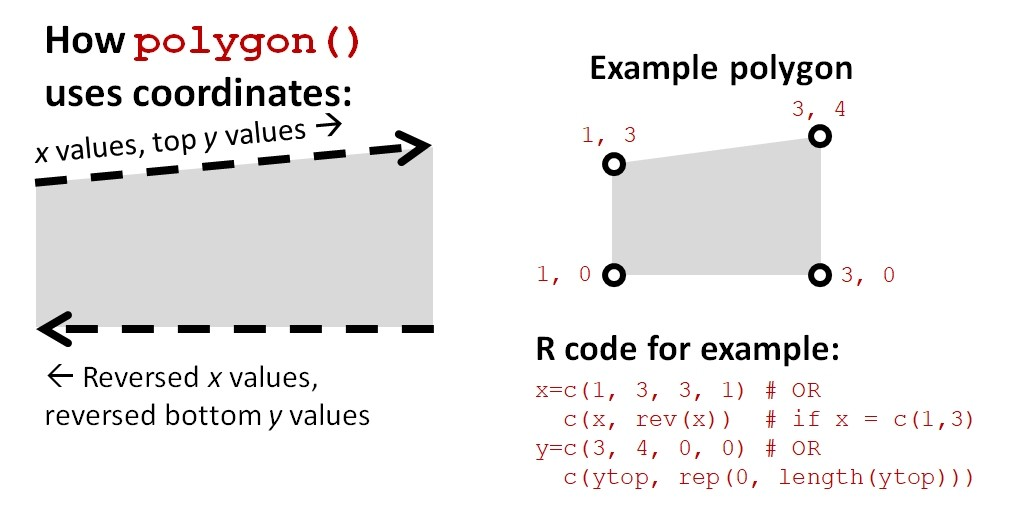
\includegraphics[keepaspectratio,alt={Diagram illustrating how the R function `polygon()` creates a filled polygon. The left panel shows a shaded polygon traced by first supplying x-coordinates and upper y-coordinates from left to right, then the x-coordinates in reverse order together with the lower y-coordinates in reverse order to close the shape. The right panel shows a four-vertex example with coordinates (1,3), (3,4), (3,0), and (1,0), along with the corresponding R code defining the x and y vectors used to draw the polygon.}]{chapters/../images/06-03.jpg}}

}

\end{figure}%

\begin{Shaded}
\begin{Highlighting}[]
\CommentTok{\# fancy plot options with par()}
\FunctionTok{par}\NormalTok{(}\AttributeTok{mfrow=}\FunctionTok{c}\NormalTok{(}\DecValTok{1}\NormalTok{,}\DecValTok{1}\NormalTok{), }\AttributeTok{mar=}\FunctionTok{c}\NormalTok{(}\FloatTok{5.1}\NormalTok{, }\FloatTok{5.1}\NormalTok{, }\FloatTok{1.1}\NormalTok{, }\FloatTok{1.1}\NormalTok{),}
    \AttributeTok{bty=}\StringTok{"n"}\NormalTok{, }\AttributeTok{lend=}\DecValTok{1}\NormalTok{,}
    \AttributeTok{las=}\DecValTok{1}\NormalTok{, }\AttributeTok{cex.axis=}\FloatTok{1.2}\NormalTok{, }\AttributeTok{cex.lab=}\FloatTok{1.2}\NormalTok{)}
\CommentTok{\# make the plot and set basic options}
\FunctionTok{plot}\NormalTok{(dx}\SpecialCharTok{$}\NormalTok{x, dx}\SpecialCharTok{$}\NormalTok{y, }\AttributeTok{type=}\StringTok{"n"}\NormalTok{,}
    \AttributeTok{ylim=}\FunctionTok{c}\NormalTok{(}\DecValTok{0}\NormalTok{, }\DecValTok{300}\NormalTok{), }\AttributeTok{xlim=}\FunctionTok{c}\NormalTok{(}\DecValTok{0}\NormalTok{, }\DecValTok{5}\NormalTok{),}
    \AttributeTok{xlab=}\StringTok{"x variable"}\NormalTok{, }\AttributeTok{ylab=}\StringTok{"y variable"}\NormalTok{)}
\CommentTok{\# make a polygon for the CRI}
\FunctionTok{polygon}\NormalTok{(}\AttributeTok{x=}\FunctionTok{c}\NormalTok{(px, }\FunctionTok{rev}\NormalTok{(px)), }\AttributeTok{y=}\FunctionTok{c}\NormalTok{(plotdf}\SpecialCharTok{$}\NormalTok{lo, }\FunctionTok{rev}\NormalTok{(plotdf}\SpecialCharTok{$}\NormalTok{up)),}
    \AttributeTok{border=}\ConstantTok{NA}\NormalTok{, }\AttributeTok{col=}\StringTok{"grey85"}\NormalTok{)}
\CommentTok{\# predicted mean}
\FunctionTok{points}\NormalTok{(plotdf}\SpecialCharTok{$}\NormalTok{x, plotdf}\SpecialCharTok{$}\NormalTok{mn, }\AttributeTok{type=}\StringTok{"l"}\NormalTok{, }\AttributeTok{lwd=}\DecValTok{2}\NormalTok{)}
\CommentTok{\# put original data on top, so not covered by }
\CommentTok{\# lines and etc.}
\FunctionTok{points}\NormalTok{(dx}\SpecialCharTok{$}\NormalTok{x, dx}\SpecialCharTok{$}\NormalTok{y, }\AttributeTok{pch=}\DecValTok{16}\NormalTok{, }\AttributeTok{cex=}\FloatTok{1.2}\NormalTok{)}
\end{Highlighting}
\end{Shaded}

\pandocbounded{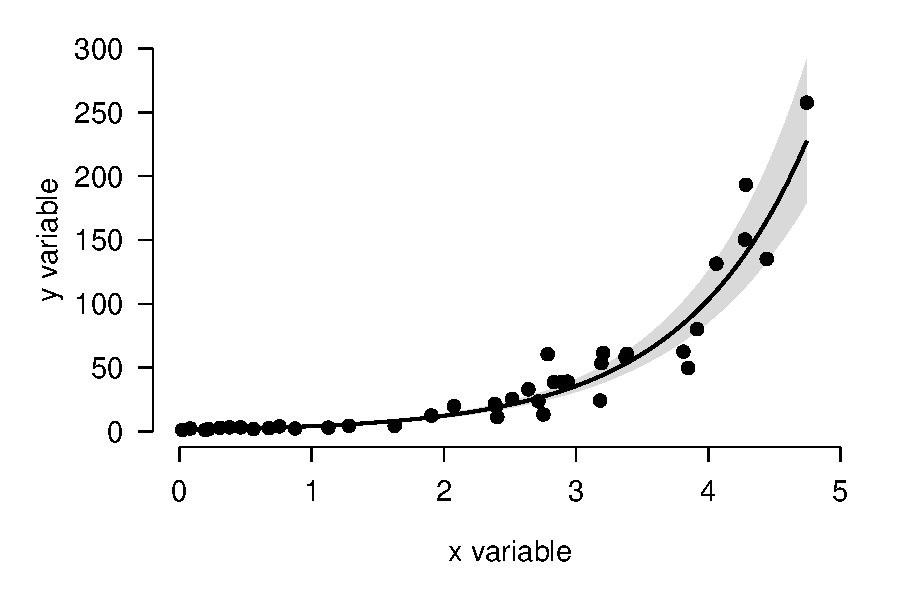
\includegraphics[keepaspectratio]{chapters/04-linear-models_files/figure-pdf/unnamed-chunk-28-1.pdf}}

\subsection{Power laws (log-log)
models}\label{power-laws-log-log-models}

The last model we'll examine is a model that appears nonlinear at first
glance, but can actually be fit as a linear model. This is power law or
allometric equation:

\[y=ax^b\]

The terms in this equation are \(a\), the value when\(x = 1\), and
\(b\), a growth constant. The sign of \(b\) determines the sign of the
slope of the curve; the magnitude of \(b\) determines how fast the
function increases or decreases.

\pandocbounded{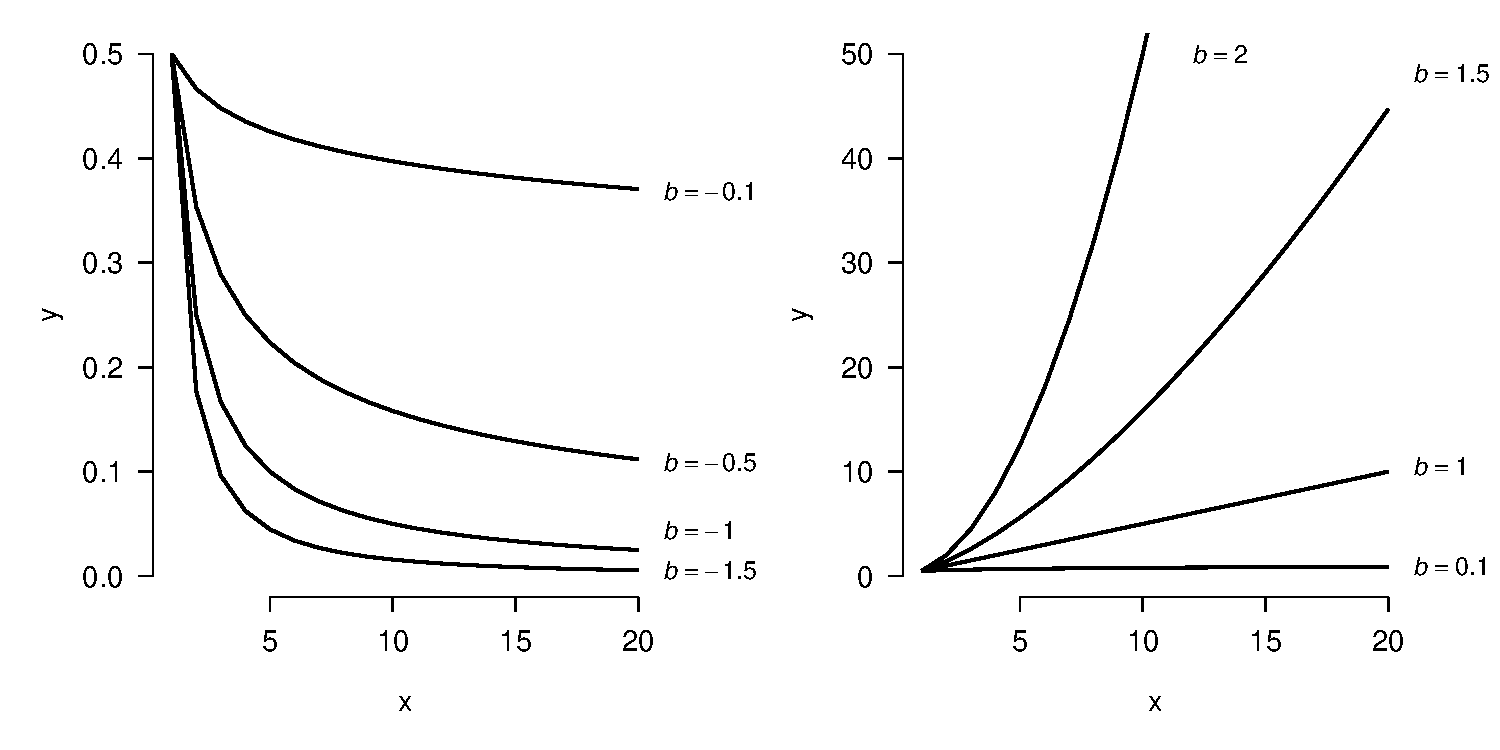
\includegraphics[keepaspectratio]{chapters/04-linear-models_files/figure-pdf/unnamed-chunk-29-1.pdf}}

While this model looks nonlinear, it can be analyzed as a linear
equation by taking advantage of some properties of logarithms. Taking
the logarithm of both sides:

\[log{\left(y\right)}=log{\left(a\right)}+blog{\left(x\right)}\]

we get an equation were \(log(y)\) is linear with respect to \(log(x)\).
Here is the previous figure on the new log-log scale. Notice how the
values on the axes are spaced, and how the lines are now straight.

\pandocbounded{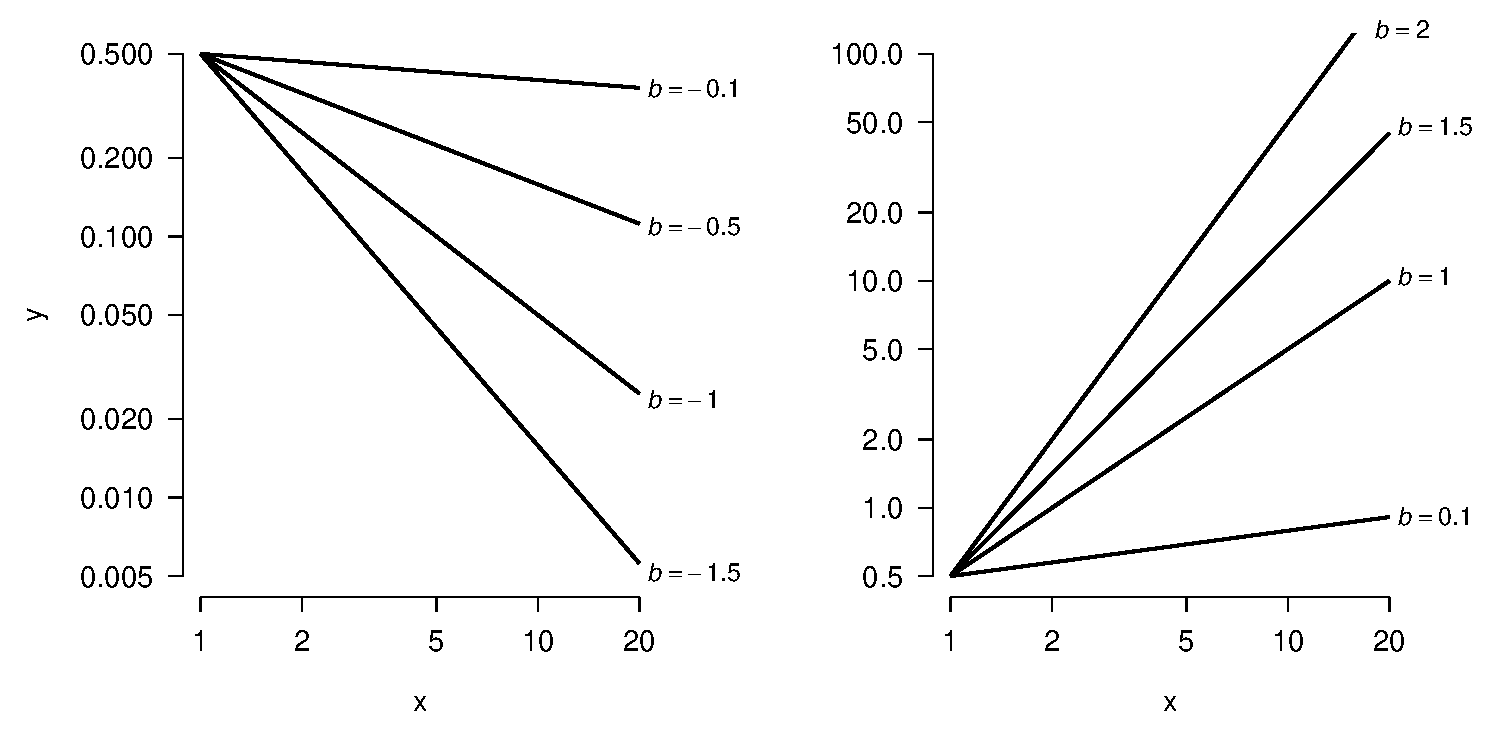
\includegraphics[keepaspectratio]{chapters/04-linear-models_files/figure-pdf/unnamed-chunk-30-1.pdf}}

What the power law and its log-transform mean is that when \(x\) is
scaled (multiplied) by some factor \(z\), \(y\) is scaled by a factor of
\(z^b\). In other words, the power law describes how proportional
changes in x relate to proportional changes in \(y\). This is because
the power law with a proportional change \(z\) to \(x\)

\[y=a\left(zx\right)^b\]

can be rearranged to:

\[y=az^bx^b\]

Taking the logarithm of both sides we can see how the linearization
works:

\[\log{\left(y\right)}=\log{(a)}+b\log{\left(z\right)}+b\log{\left(x\right)}\]

In its transformed state, we see that \(log(y)\) is linear with respect
to both \(log(z)\) and \(log(x)\). This can be simplified by factoring
out b out of the terms that contain it, to get the linearized power law
with slope \(b\).

\[\log{\left(y\right)}=\log{(a)}+b\left(\log{\left(z\right)}+\log{\left(x\right)}\right)\]

This shows that multiplying \(x\) times a factor \(z\) is equivalent to
adding \(log(z)\) to \(log(x)\). This is one of the definitions of the
logarithm. This is also why the effect of \(x\) on \(y\) is linear on
the log-log scale but curved on the linear-linear scale.

Transforming the power law model to linearize it will get you the same
parameter estimates, but with the benefit of being able to use the ease
and convenience of linear models. The hardest part of fitting this model
in JAGS is keeping track of which values are on the log scale and which
values are not. Complicating this is the fact that JAGS and BUGS handle
data transformations differently (Lunn et al.~2000, Plummer 2003).

\textbf{BUGS vs.~JAGS}

BUGS (WinBUGS and OpenBUGS) was a predecessor to JAGS. Most published
textbooks, and online help examples, are old enough to have been written
in BUGS. There are very few differences between BUGS and JAGS, and this
issue with data transformation is probably one of the most important.
The model script here should work in BUGS as well as JAGS, but the
old-style BUGS equivalent might not work in JAGS. This took me a long
time to figure out when I was writing this module.

As with the log-linear model, we have two options for how to code the
linearized power law. Method 1 is to model \(y\) on its original scale
with a lognormal distribution. Method 2 is to transform \(y\) in a data
block and use a normal distribution. Both methods will get you the same
answer.

\subsubsection{Power law option 1: lognormal
y}\label{power-law-option-1-lognormal-y}

\begin{Shaded}
\begin{Highlighting}[]
\CommentTok{\# simulate some data}
\FunctionTok{set.seed}\NormalTok{(}\DecValTok{42}\NormalTok{)}
\NormalTok{n }\OtherTok{\textless{}{-}} \DecValTok{30}
\NormalTok{dx }\OtherTok{\textless{}{-}} \FunctionTok{data.frame}\NormalTok{(}\AttributeTok{x=}\FunctionTok{runif}\NormalTok{(n, }\DecValTok{0}\NormalTok{, }\DecValTok{20}\NormalTok{))}

\NormalTok{A }\OtherTok{\textless{}{-}} \FloatTok{2.1}
\NormalTok{logA }\OtherTok{\textless{}{-}} \FunctionTok{log}\NormalTok{(A)}
\NormalTok{B }\OtherTok{\textless{}{-}} \FloatTok{1.5}
\NormalTok{sigma.res }\OtherTok{\textless{}{-}} \FloatTok{0.3}
\NormalTok{dx}\SpecialCharTok{$}\NormalTok{y }\OtherTok{\textless{}{-}} \FunctionTok{exp}\NormalTok{(logA }\SpecialCharTok{+}\NormalTok{ B}\SpecialCharTok{*}\FunctionTok{log}\NormalTok{(dx}\SpecialCharTok{$}\NormalTok{x) }\SpecialCharTok{+} \FunctionTok{rnorm}\NormalTok{(n, }\DecValTok{0}\NormalTok{, sigma.res))}

\CommentTok{\# MUST be TRUE:}
\FunctionTok{all}\NormalTok{(dx}\SpecialCharTok{$}\NormalTok{y }\SpecialCharTok{\textgreater{}} \DecValTok{0}\NormalTok{)}
\end{Highlighting}
\end{Shaded}

\begin{verbatim}
[1] TRUE
\end{verbatim}

\begin{Shaded}
\begin{Highlighting}[]
\CommentTok{\# power law (allometric equation)}
\NormalTok{mod.name }\OtherTok{\textless{}{-}} \StringTok{"jags\_power\_law.txt"}
\FunctionTok{sink}\NormalTok{(mod.name)}
\FunctionTok{cat}\NormalTok{(}\StringTok{"}
\StringTok{    model\{}
\StringTok{        \# priors}
\StringTok{        \#\# intercept}
\StringTok{        logA \textasciitilde{} dnorm(0, 0.001)}

\StringTok{        \#\# growth constant}
\StringTok{        B \textasciitilde{} dnorm(0, 0.001)}

\StringTok{        \#\# residual SD and precision}
\StringTok{        sigma \textasciitilde{} dlnorm(1, 0.25)}
\StringTok{        tau \textless{}{-} 1 / (sigma\^{}2)}

\StringTok{        \# likelihood}
\StringTok{        for(i in 1:n)\{}
\StringTok{            \# expected value on LOG scale}
\StringTok{            eta[i] \textless{}{-} logA +  B * log(x[i])}
\StringTok{            y[i] \textasciitilde{} dlnorm(eta[i], tau)}
\StringTok{        \}\#i}

\StringTok{        \# derived quantity: original scale A}
\StringTok{        A \textless{}{-} exp(logA)        }

\StringTok{    \}\#model}

\StringTok{"}\NormalTok{, }\AttributeTok{fill=}\ConstantTok{TRUE}\NormalTok{)}
\FunctionTok{sink}\NormalTok{()}

\CommentTok{\# parameters to monitor}
\NormalTok{params }\OtherTok{\textless{}{-}} \FunctionTok{c}\NormalTok{(}\StringTok{"A"}\NormalTok{, }\StringTok{"B"}\NormalTok{, }\StringTok{"sigma"}\NormalTok{)}

\CommentTok{\# MCMC parameters}
\NormalTok{n.iter }\OtherTok{\textless{}{-}} \FloatTok{5e4}
\NormalTok{n.burnin }\OtherTok{\textless{}{-}} \FloatTok{1e4}
\NormalTok{n.thin }\OtherTok{\textless{}{-}} \DecValTok{100}
\NormalTok{nchains }\OtherTok{\textless{}{-}} \DecValTok{3}

\CommentTok{\# package data for JAGS}
\NormalTok{in.data }\OtherTok{\textless{}{-}} \FunctionTok{list}\NormalTok{(}\AttributeTok{y=}\NormalTok{dx}\SpecialCharTok{$}\NormalTok{y,}
    \AttributeTok{n=}\NormalTok{n, }\AttributeTok{x=}\NormalTok{dx}\SpecialCharTok{$}\NormalTok{x)}

\CommentTok{\# function to define initial values for MCMC chains}
\NormalTok{init.fun }\OtherTok{\textless{}{-}} \ControlFlowTok{function}\NormalTok{(nc)\{}
\NormalTok{    res }\OtherTok{\textless{}{-}} \FunctionTok{vector}\NormalTok{(}\StringTok{"list"}\NormalTok{, }\AttributeTok{length=}\NormalTok{nc)}
    \ControlFlowTok{for}\NormalTok{(i }\ControlFlowTok{in} \DecValTok{1}\SpecialCharTok{:}\NormalTok{nc)\{}
\NormalTok{        res[[i]] }\OtherTok{\textless{}{-}} \FunctionTok{list}\NormalTok{(}\AttributeTok{logA=}\FunctionTok{rnorm}\NormalTok{(}\DecValTok{1}\NormalTok{, }\DecValTok{0}\NormalTok{, }\DecValTok{100}\NormalTok{),}
                         \AttributeTok{B=}\FunctionTok{rnorm}\NormalTok{(}\DecValTok{1}\NormalTok{, }\DecValTok{0}\NormalTok{, }\DecValTok{100}\NormalTok{),}
                         \AttributeTok{sigma=}\FunctionTok{rlnorm}\NormalTok{(}\DecValTok{1}\NormalTok{, }\DecValTok{1}\NormalTok{, }\DecValTok{2}\NormalTok{))}
\NormalTok{    \}}
    \FunctionTok{return}\NormalTok{(res)}
\NormalTok{\}}
\NormalTok{inits }\OtherTok{\textless{}{-}} \FunctionTok{init.fun}\NormalTok{(nchains)}

\CommentTok{\# fit model}
\NormalTok{mod13 }\OtherTok{\textless{}{-}} \FunctionTok{jags}\NormalTok{(}\AttributeTok{data=}\NormalTok{in.data, }\AttributeTok{inits=}\NormalTok{inits,}
              \AttributeTok{parameters.to.save=}\NormalTok{params,}
              \AttributeTok{model.file=}\NormalTok{mod.name,}
              \AttributeTok{n.chains=}\NormalTok{nchains, }\AttributeTok{n.iter=}\NormalTok{n.iter,}
              \AttributeTok{n.burnin=}\NormalTok{n.burnin, }\AttributeTok{n.thin=}\NormalTok{n.thin)}\CommentTok{\#jags}
\end{Highlighting}
\end{Shaded}

\begin{verbatim}
Compiling model graph
   Resolving undeclared variables
   Allocating nodes
Graph information:
   Observed stochastic nodes: 30
   Unobserved stochastic nodes: 3
   Total graph size: 162

Initializing model
\end{verbatim}

\begin{Shaded}
\begin{Highlighting}[]
\NormalTok{mod13}
\end{Highlighting}
\end{Shaded}

\begin{verbatim}
Inference for Bugs model at "jags_power_law.txt", fit using jags,
 3 chains, each with 50000 iterations (first 10000 discarded), n.thin = 100
 n.sims = 1200 iterations saved. Running time = 11.11 secs
         mu.vect sd.vect    2.5%     25%     50%     75%   97.5%  Rhat n.eff
A          2.248   0.558   1.325   1.852   2.169   2.580   3.473 1.000  1200
B          1.439   0.100   1.243   1.374   1.439   1.509   1.641 1.000  1200
sigma      0.367   0.051   0.283   0.331   0.362   0.395   0.479 1.002   930
deviance 272.060   2.577 269.198 270.185 271.395 273.214 278.616 1.001  1200

For each parameter, n.eff is a crude measure of effective sample size,
and Rhat is the potential scale reduction factor (at convergence, Rhat=1).

DIC info (using the rule: pV = var(deviance)/2)
pV = 3.3 and DIC = 275.4
DIC is an estimate of expected predictive error (lower deviance is better).
\end{verbatim}

\subsubsection{Power law option 2:
linearized}\label{power-law-option-2-linearized}

The equivalent approach is to handle the transformation of \(y\) in a
separate data block. Either way is fine; I would probably use Method 1
in my own work because it's a little simpler.

Here's the alternative method. Only the model file has changed;
everything else is the same. The alternative method uses a data block to
transform the \(y\) values in the input, and uses a normal distribution
to relate the expected value \texttt{eta} to the observed value
\texttt{z}. The method above uses the lognormal distribution, which
effectively undoes the log transform of y which was implied by the fact
that the deterministic part of the model was on the log scale.

\begin{Shaded}
\begin{Highlighting}[]
\CommentTok{\# power law (allometric equation) with}
\CommentTok{\# transformation in data block}
\NormalTok{mod.name }\OtherTok{\textless{}{-}} \StringTok{"jags\_power\_law\_v2.txt"}
\FunctionTok{sink}\NormalTok{(mod.name)}
\FunctionTok{cat}\NormalTok{(}\StringTok{"}
\StringTok{    data\{}
\StringTok{        for(i in 1:n)\{z[i] \textless{}{-} log(y[i])\}\#i}
\StringTok{    \}}

\StringTok{    model\{}
\StringTok{        \# priors}
\StringTok{        \#\# intercept}
\StringTok{        logA \textasciitilde{} dnorm(0, 0.001)}

\StringTok{        \#\# growth constant}
\StringTok{        B \textasciitilde{} dnorm(0, 0.001)}

\StringTok{        \#\# residual SD and precision}
\StringTok{        sigma \textasciitilde{} dlnorm(1, 0.25)}
\StringTok{        tau \textless{}{-} 1 / (sigma\^{}2)}

\StringTok{        \# likelihood}
\StringTok{        for(i in 1:n)\{}
\StringTok{            \# expected value on LOG scale}
\StringTok{            eta[i] \textless{}{-} logA +  B * log(x[i])}
\StringTok{            \# NOTE: likelihood uses transformed z, not y}
\StringTok{            \# and dnorm(), not dlnorm()}
\StringTok{            z[i] \textasciitilde{} dnorm(eta[i], tau)}
\StringTok{        \}\#i}

\StringTok{        \# derived quantity: original scale A}
\StringTok{        A \textless{}{-} exp(logA)        }

\StringTok{    \}\#model}

\StringTok{"}\NormalTok{, }\AttributeTok{fill=}\ConstantTok{TRUE}\NormalTok{)}
\FunctionTok{sink}\NormalTok{()}

\CommentTok{\# parameters to monitor}
\NormalTok{params }\OtherTok{\textless{}{-}} \FunctionTok{c}\NormalTok{(}\StringTok{"A"}\NormalTok{, }\StringTok{"B"}\NormalTok{, }\StringTok{"sigma"}\NormalTok{)}

\CommentTok{\# MCMC parameters}
\NormalTok{n.iter }\OtherTok{\textless{}{-}} \FloatTok{5e4}
\NormalTok{n.burnin }\OtherTok{\textless{}{-}} \FloatTok{1e4}
\NormalTok{n.thin }\OtherTok{\textless{}{-}} \DecValTok{100}
\NormalTok{nchains }\OtherTok{\textless{}{-}} \DecValTok{3}

\CommentTok{\# package data for JAGS}
\NormalTok{in.data }\OtherTok{\textless{}{-}} \FunctionTok{list}\NormalTok{(}\AttributeTok{y=}\NormalTok{dx}\SpecialCharTok{$}\NormalTok{y,}
    \AttributeTok{n=}\NormalTok{n, }\AttributeTok{x=}\NormalTok{dx}\SpecialCharTok{$}\NormalTok{x)}

\CommentTok{\# function to define initial values for MCMC chains}
\NormalTok{init.fun }\OtherTok{\textless{}{-}} \ControlFlowTok{function}\NormalTok{(nc)\{}
\NormalTok{    res }\OtherTok{\textless{}{-}} \FunctionTok{vector}\NormalTok{(}\StringTok{"list"}\NormalTok{, }\AttributeTok{length=}\NormalTok{nc)}
    \ControlFlowTok{for}\NormalTok{(i }\ControlFlowTok{in} \DecValTok{1}\SpecialCharTok{:}\NormalTok{nc)\{}
\NormalTok{        res[[i]] }\OtherTok{\textless{}{-}} \FunctionTok{list}\NormalTok{(}\AttributeTok{logA=}\FunctionTok{rnorm}\NormalTok{(}\DecValTok{1}\NormalTok{, }\DecValTok{0}\NormalTok{, }\DecValTok{100}\NormalTok{),}
                         \AttributeTok{B=}\FunctionTok{rnorm}\NormalTok{(}\DecValTok{1}\NormalTok{, }\DecValTok{0}\NormalTok{, }\DecValTok{100}\NormalTok{),}
                         \AttributeTok{sigma=}\FunctionTok{rlnorm}\NormalTok{(}\DecValTok{1}\NormalTok{, }\DecValTok{1}\NormalTok{, }\DecValTok{2}\NormalTok{))}
\NormalTok{    \}}
    \FunctionTok{return}\NormalTok{(res)}
\NormalTok{\}}
\NormalTok{inits }\OtherTok{\textless{}{-}} \FunctionTok{init.fun}\NormalTok{(nchains)}

\CommentTok{\# fit model}
\NormalTok{mod13v2 }\OtherTok{\textless{}{-}} \FunctionTok{jags}\NormalTok{(}\AttributeTok{data=}\NormalTok{in.data, }\AttributeTok{inits=}\NormalTok{inits,}
              \AttributeTok{parameters.to.save=}\NormalTok{params,}
              \AttributeTok{model.file=}\NormalTok{mod.name,}
              \AttributeTok{n.chains=}\NormalTok{nchains, }\AttributeTok{n.iter=}\NormalTok{n.iter,}
              \AttributeTok{n.burnin=}\NormalTok{n.burnin, }\AttributeTok{n.thin=}\NormalTok{n.thin)}\CommentTok{\#jags}
\end{Highlighting}
\end{Shaded}

\begin{verbatim}
Compiling data graph
   Resolving undeclared variables
   Allocating nodes
   Initializing
   Reading data back into data table
Compiling model graph
   Resolving undeclared variables
   Allocating nodes
Graph information:
   Observed stochastic nodes: 30
   Unobserved stochastic nodes: 3
   Total graph size: 192

Initializing model
\end{verbatim}

\begin{Shaded}
\begin{Highlighting}[]
\NormalTok{mod13v2}
\end{Highlighting}
\end{Shaded}

\begin{verbatim}
Inference for Bugs model at "jags_power_law_v2.txt", fit using jags,
 3 chains, each with 50000 iterations (first 10000 discarded), n.thin = 100
 n.sims = 1200 iterations saved. Running time = 3.69 secs
         mu.vect sd.vect   2.5%    25%    50%    75%  97.5%  Rhat n.eff
A          2.263   0.544  1.380  1.885  2.213  2.551  3.543 1.001  1200
B          1.437   0.096  1.244  1.374  1.436  1.500  1.618 1.000  1200
sigma      0.369   0.052  0.289  0.332  0.360  0.399  0.485 1.001  1200
deviance  24.015   2.580 21.140 22.168 23.355 25.144 30.715 1.002  1200

For each parameter, n.eff is a crude measure of effective sample size,
and Rhat is the potential scale reduction factor (at convergence, Rhat=1).

DIC info (using the rule: pV = var(deviance)/2)
pV = 3.3 and DIC = 27.3
DIC is an estimate of expected predictive error (lower deviance is better).
\end{verbatim}

\subsubsection{Plotting power laws}\label{plotting-power-laws}

Getting predicted values for the Bayesian linearized power law fit is
very similar to the process for the log-linear model. We just have to
make sure to use the correct equation, and keep track of what is on the
log scale and what is on the linear scale. Below we see two methods:
Method 1 calculates y directly on the linear (untransformed) scale using
the model output A (which we included in the model as a derived
quantity). Method 2 calculates log(y) using log(A), then exponentiates
to get the linear scale predictions. Both methods work just fine. In my
own work I'd probably use Method 1 unless I had a compelling reason not
to.

\paragraph{Method 1: predict y on linear
scale}\label{method-1-predict-y-on-linear-scale}

\begin{Shaded}
\begin{Highlighting}[]
\CommentTok{\# matrix of coefficients}
\NormalTok{prx }\OtherTok{\textless{}{-}}\NormalTok{ mod13}\SpecialCharTok{$}\NormalTok{BUGSoutput}\SpecialCharTok{$}\NormalTok{sims.matrix}
\DocumentationTok{\#\# don\textquotesingle{}t need deviance or sigma}
\NormalTok{prx }\OtherTok{\textless{}{-}}\NormalTok{ prx[,}\FunctionTok{c}\NormalTok{(}\StringTok{"A"}\NormalTok{, }\StringTok{"B"}\NormalTok{)]}
\NormalTok{post.n }\OtherTok{\textless{}{-}} \FunctionTok{nrow}\NormalTok{(prx)}

\CommentTok{\# x values at which to predict}
\NormalTok{pred.n }\OtherTok{\textless{}{-}} \DecValTok{100}
\NormalTok{px }\OtherTok{\textless{}{-}} \FunctionTok{seq}\NormalTok{(}\FunctionTok{min}\NormalTok{(dx}\SpecialCharTok{$}\NormalTok{x), }\FunctionTok{max}\NormalTok{(dx}\SpecialCharTok{$}\NormalTok{x), }\AttributeTok{length=}\NormalTok{pred.n)}

\CommentTok{\# set up matrix}
\NormalTok{pred.mat }\OtherTok{\textless{}{-}} \FunctionTok{matrix}\NormalTok{(}\ConstantTok{NA}\NormalTok{, }\AttributeTok{nrow=}\NormalTok{pred.n, }\AttributeTok{ncol=}\NormalTok{post.n)}

\CommentTok{\# fill in a loop}
\ControlFlowTok{for}\NormalTok{(i }\ControlFlowTok{in} \DecValTok{1}\SpecialCharTok{:}\NormalTok{post.n)\{}
\NormalTok{    pred.mat[,i] }\OtherTok{\textless{}{-}}\NormalTok{ prx[i,}\StringTok{"A"}\NormalTok{] }\SpecialCharTok{*}\NormalTok{ px}\SpecialCharTok{\^{}}\NormalTok{prx[i,}\StringTok{"B"}\NormalTok{]}
\NormalTok{\}}\CommentTok{\#i}

\CommentTok{\# set up data frame with mean and CRI}
\CommentTok{\# }\AlertTok{NOTE}\CommentTok{: don\textquotesingle{}t need to exponentiate, because we}
\CommentTok{\#       have linear{-}scale A and can thus }
\CommentTok{\#       calculate linear{-}scale y directly.}
\NormalTok{plotdf }\OtherTok{\textless{}{-}} \FunctionTok{data.frame}\NormalTok{(}\AttributeTok{x=}\NormalTok{px,}
    \AttributeTok{mn=}\FunctionTok{apply}\NormalTok{(pred.mat, }\DecValTok{1}\NormalTok{, mean),}
    \AttributeTok{lo=}\FunctionTok{apply}\NormalTok{(pred.mat, }\DecValTok{1}\NormalTok{, quantile, }\FloatTok{0.025}\NormalTok{),}
    \AttributeTok{up=}\FunctionTok{apply}\NormalTok{(pred.mat, }\DecValTok{1}\NormalTok{, quantile, }\FloatTok{0.975}\NormalTok{))}

\CommentTok{\# fancy plot options with par()}
\FunctionTok{par}\NormalTok{(}\AttributeTok{mfrow=}\FunctionTok{c}\NormalTok{(}\DecValTok{1}\NormalTok{,}\DecValTok{1}\NormalTok{), }\AttributeTok{mar=}\FunctionTok{c}\NormalTok{(}\FloatTok{5.1}\NormalTok{, }\FloatTok{5.1}\NormalTok{, }\FloatTok{1.1}\NormalTok{, }\FloatTok{1.1}\NormalTok{),}
    \AttributeTok{bty=}\StringTok{"n"}\NormalTok{, }\AttributeTok{lend=}\DecValTok{1}\NormalTok{,}
    \AttributeTok{las=}\DecValTok{1}\NormalTok{, }\AttributeTok{cex.axis=}\FloatTok{1.2}\NormalTok{, }\AttributeTok{cex.lab=}\FloatTok{1.2}\NormalTok{)}
\CommentTok{\# make the plot and set basic options}
\FunctionTok{plot}\NormalTok{(dx}\SpecialCharTok{$}\NormalTok{x, dx}\SpecialCharTok{$}\NormalTok{y, }\AttributeTok{type=}\StringTok{"n"}\NormalTok{,}
    \AttributeTok{ylim=}\FunctionTok{c}\NormalTok{(}\DecValTok{0}\NormalTok{, }\DecValTok{200}\NormalTok{), }\AttributeTok{xlim=}\FunctionTok{c}\NormalTok{(}\DecValTok{0}\NormalTok{, }\DecValTok{20}\NormalTok{),}
    \AttributeTok{xlab=}\StringTok{"x variable"}\NormalTok{, }\AttributeTok{ylab=}\StringTok{"y variable"}\NormalTok{)}
\CommentTok{\# make a polygon for the CRI}
\FunctionTok{polygon}\NormalTok{(}\AttributeTok{x=}\FunctionTok{c}\NormalTok{(px, }\FunctionTok{rev}\NormalTok{(px)), }\AttributeTok{y=}\FunctionTok{c}\NormalTok{(plotdf}\SpecialCharTok{$}\NormalTok{lo, }\FunctionTok{rev}\NormalTok{(plotdf}\SpecialCharTok{$}\NormalTok{up)),}
    \AttributeTok{border=}\ConstantTok{NA}\NormalTok{, }\AttributeTok{col=}\StringTok{"grey85"}\NormalTok{)}
\CommentTok{\# predicted mean}
\FunctionTok{points}\NormalTok{(plotdf}\SpecialCharTok{$}\NormalTok{x, plotdf}\SpecialCharTok{$}\NormalTok{mn, }\AttributeTok{type=}\StringTok{"l"}\NormalTok{, }\AttributeTok{lwd=}\DecValTok{2}\NormalTok{)}
\CommentTok{\# put original data on top, so not covered by }
\CommentTok{\# lines and etc.}
\FunctionTok{points}\NormalTok{(dx}\SpecialCharTok{$}\NormalTok{x, dx}\SpecialCharTok{$}\NormalTok{y, }\AttributeTok{pch=}\DecValTok{16}\NormalTok{, }\AttributeTok{cex=}\FloatTok{1.2}\NormalTok{)}
\end{Highlighting}
\end{Shaded}

\pandocbounded{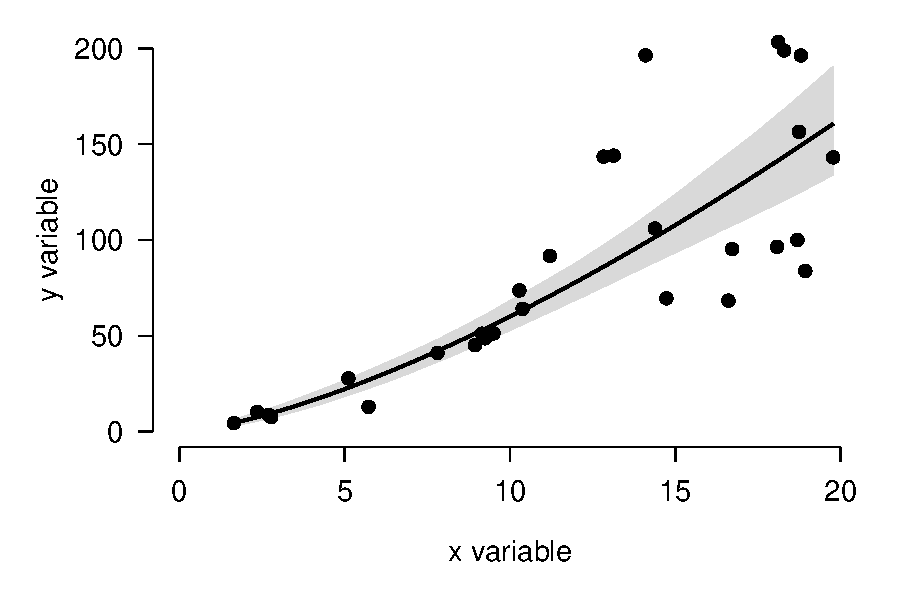
\includegraphics[keepaspectratio]{chapters/04-linear-models_files/figure-pdf/unnamed-chunk-31-1.pdf}}

\paragraph{Method 2: predict y on log
scale}\label{method-2-predict-y-on-log-scale}

Oops, we forgot to calculate the linear scale A in our model and don't
feel like going back to re-run the model. That's fine, we can just
generate predictions on the log-log scale and backtransform . Very
little in the code below is changed from Method 1: the prediction
equation for \texttt{pred.mat{[},i{]}} is linear, and the results are
exponentiated with \texttt{exp()}.

\begin{Shaded}
\begin{Highlighting}[]
\CommentTok{\# matrix of coefficients}
\NormalTok{prx }\OtherTok{\textless{}{-}}\NormalTok{ mod13}\SpecialCharTok{$}\NormalTok{BUGSoutput}\SpecialCharTok{$}\NormalTok{sims.matrix}
\DocumentationTok{\#\# don\textquotesingle{}t need deviance or sigma}
\NormalTok{prx }\OtherTok{\textless{}{-}}\NormalTok{ prx[,}\FunctionTok{c}\NormalTok{(}\StringTok{"A"}\NormalTok{, }\StringTok{"B"}\NormalTok{)]}

\DocumentationTok{\#\# OOPS, we forgot to get linear{-}scale A}
\DocumentationTok{\#\# in the model, and don\textquotesingle{}t feel like }
\DocumentationTok{\#\# re{-}running it. This line will get us}
\DocumentationTok{\#\# the log{-}scale A posteriors.}
\NormalTok{prx[,}\StringTok{"A"}\NormalTok{] }\OtherTok{\textless{}{-}} \FunctionTok{log}\NormalTok{(prx[,}\StringTok{"A"}\NormalTok{])}

\NormalTok{post.n }\OtherTok{\textless{}{-}} \FunctionTok{nrow}\NormalTok{(prx)}

\CommentTok{\# x values at which to predict}
\NormalTok{pred.n }\OtherTok{\textless{}{-}} \DecValTok{100}
\NormalTok{px }\OtherTok{\textless{}{-}} \FunctionTok{seq}\NormalTok{(}\FunctionTok{min}\NormalTok{(dx}\SpecialCharTok{$}\NormalTok{x), }\FunctionTok{max}\NormalTok{(dx}\SpecialCharTok{$}\NormalTok{x), }\AttributeTok{length=}\NormalTok{pred.n)}

\CommentTok{\# set up matrix}
\NormalTok{pred.mat }\OtherTok{\textless{}{-}} \FunctionTok{matrix}\NormalTok{(}\ConstantTok{NA}\NormalTok{, }\AttributeTok{nrow=}\NormalTok{pred.n, }\AttributeTok{ncol=}\NormalTok{post.n)}

\CommentTok{\# fill in a loop}
\CommentTok{\# }\AlertTok{NOTE}\CommentTok{: we are predicting on log{-}log scale, }
\CommentTok{\#       so don\textquotesingle{}t forget to log{-}transform x!}
\ControlFlowTok{for}\NormalTok{(i }\ControlFlowTok{in} \DecValTok{1}\SpecialCharTok{:}\NormalTok{post.n)\{}
\NormalTok{    pred.mat[,i] }\OtherTok{\textless{}{-}}\NormalTok{ prx[i,}\StringTok{"A"}\NormalTok{] }\SpecialCharTok{+} \FunctionTok{log}\NormalTok{(px) }\SpecialCharTok{*}\NormalTok{ prx[i,}\StringTok{"B"}\NormalTok{]}
\NormalTok{\}}\CommentTok{\#i}

\CommentTok{\# set up data frame with mean and CRI}
\CommentTok{\# }\AlertTok{NOTE}\CommentTok{: need to exponentiate, because }
\CommentTok{\#       predictions are on log scale.}
\NormalTok{plotdf }\OtherTok{\textless{}{-}} \FunctionTok{data.frame}\NormalTok{(}\AttributeTok{x=}\NormalTok{px,}
    \AttributeTok{mn=}\FunctionTok{exp}\NormalTok{(}\FunctionTok{apply}\NormalTok{(pred.mat, }\DecValTok{1}\NormalTok{, mean)),}
    \AttributeTok{lo=}\FunctionTok{exp}\NormalTok{(}\FunctionTok{apply}\NormalTok{(pred.mat, }\DecValTok{1}\NormalTok{, quantile, }\FloatTok{0.025}\NormalTok{)),}
    \AttributeTok{up=}\FunctionTok{exp}\NormalTok{(}\FunctionTok{apply}\NormalTok{(pred.mat, }\DecValTok{1}\NormalTok{, quantile, }\FloatTok{0.975}\NormalTok{)))}

\CommentTok{\# fancy plot options with par()}
\FunctionTok{par}\NormalTok{(}\AttributeTok{mfrow=}\FunctionTok{c}\NormalTok{(}\DecValTok{1}\NormalTok{,}\DecValTok{1}\NormalTok{), }\AttributeTok{mar=}\FunctionTok{c}\NormalTok{(}\FloatTok{5.1}\NormalTok{, }\FloatTok{5.1}\NormalTok{, }\FloatTok{1.1}\NormalTok{, }\FloatTok{1.1}\NormalTok{),}
    \AttributeTok{bty=}\StringTok{"n"}\NormalTok{, }\AttributeTok{lend=}\DecValTok{1}\NormalTok{,}
    \AttributeTok{las=}\DecValTok{1}\NormalTok{, }\AttributeTok{cex.axis=}\FloatTok{1.2}\NormalTok{, }\AttributeTok{cex.lab=}\FloatTok{1.2}\NormalTok{)}
\CommentTok{\# make the plot and set basic options}
\FunctionTok{plot}\NormalTok{(dx}\SpecialCharTok{$}\NormalTok{x, dx}\SpecialCharTok{$}\NormalTok{y, }\AttributeTok{type=}\StringTok{"n"}\NormalTok{,}
    \AttributeTok{ylim=}\FunctionTok{c}\NormalTok{(}\DecValTok{0}\NormalTok{, }\DecValTok{200}\NormalTok{), }\AttributeTok{xlim=}\FunctionTok{c}\NormalTok{(}\DecValTok{0}\NormalTok{, }\DecValTok{20}\NormalTok{),}
    \AttributeTok{xlab=}\StringTok{"x variable"}\NormalTok{, }\AttributeTok{ylab=}\StringTok{"y variable"}\NormalTok{)}
\CommentTok{\# make a polygon for the CRI}
\FunctionTok{polygon}\NormalTok{(}\AttributeTok{x=}\FunctionTok{c}\NormalTok{(px, }\FunctionTok{rev}\NormalTok{(px)), }\AttributeTok{y=}\FunctionTok{c}\NormalTok{(plotdf}\SpecialCharTok{$}\NormalTok{lo, }\FunctionTok{rev}\NormalTok{(plotdf}\SpecialCharTok{$}\NormalTok{up)),}
    \AttributeTok{border=}\ConstantTok{NA}\NormalTok{, }\AttributeTok{col=}\StringTok{"grey85"}\NormalTok{)}
\CommentTok{\# predicted mean}
\FunctionTok{points}\NormalTok{(plotdf}\SpecialCharTok{$}\NormalTok{x, plotdf}\SpecialCharTok{$}\NormalTok{mn, }\AttributeTok{type=}\StringTok{"l"}\NormalTok{, }\AttributeTok{lwd=}\DecValTok{2}\NormalTok{)}
\CommentTok{\# put original data on top, so not covered by }
\CommentTok{\# lines and etc.}
\FunctionTok{points}\NormalTok{(dx}\SpecialCharTok{$}\NormalTok{x, dx}\SpecialCharTok{$}\NormalTok{y, }\AttributeTok{pch=}\DecValTok{16}\NormalTok{, }\AttributeTok{cex=}\FloatTok{1.2}\NormalTok{)}
\end{Highlighting}
\end{Shaded}

\pandocbounded{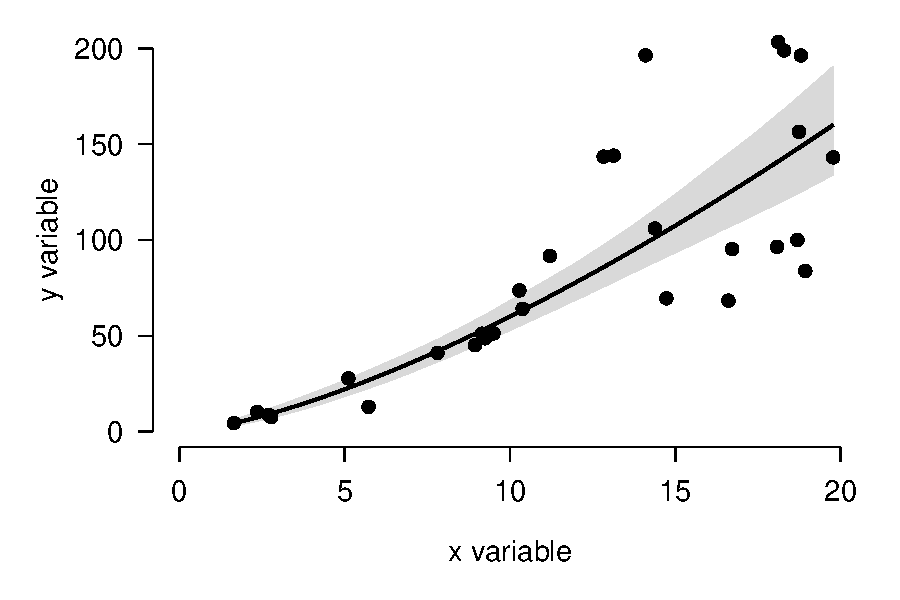
\includegraphics[keepaspectratio]{chapters/04-linear-models_files/figure-pdf/unnamed-chunk-32-1.pdf}}

The plot from Method 2 is exactly the same as the plot for Method 1.
This illustrates the freedom that comes with understanding your model
and the various ways it can be expressed.

\section{Conclusions}\label{conclusions}

Now that you have seen the ways we fit linear models in JAGS, you should
have both a better understanding of linear models and Bayesian model
fitting. In particular, wrapping your head around the ANCOVA models
should set you up to understand one of the more advanced topics in this
course, mixed models. It only takes one subtle change to convert an
ANCOVA into a mixed model.

Likewise, understanding how the linear regression model was put together
will help you understand the generalized linear model (GLM). The GLM
generalized the linear model by allowing the response distribution to be
something other than the normal, and allowing a \textbf{link} function
that relates the scale of the response variable and the scale of the
deterministic part of the model. Both of these changes are very
straightforward in JAGS\ldots much more so than in R!

\chapter{GLM for count data}\label{sec-glm1}

\chapter{GLM for binomial data}\label{sec-glm2}

\chapter{GLM for continuous data}\label{sec-glm3}

\chapter{Nonlinear models in JAGS}\label{sec-non}

\chapter{Mixed models and random effects}\label{sec-mixed}

\part{Special applications of Bayesian inference}

State space state space state space\ldots{}

\chapter{}\label{section}

\chapter{State space models}\label{sec-state}

\bookmarksetup{startatroot}

\chapter*{References}\label{references}
\addcontentsline{toc}{chapter}{References}

\markboth{References}{References}

\protect\phantomsection\label{refs}




\end{document}
